\documentclass[11pt,letterpaper]{book}
\usepackage[utf8]{inputenc}
\usepackage[spanish]{babel}
\usepackage{graphicx}
\usepackage{subfigure}

\usepackage[top=1in, bottom=1in, right=1in, left=1in]{geometry}

%Paqueteria del glosario
\usepackage[hidelinks]{hyperref}
\usepackage[toc,style=altlistgroup,hyperfirst=false]{glossaries}
\makeindex
\makeglossaries

%%FORMATO PARA INGRESAR DEFINICION
%%%  \newglossaryentry{nombre} %como será escrito en el texto
%%%   {
%%%	   name={Nombre}, %como será escrito en el %%%   glosario
%%%	   description={aquí defines que es nombre}
%%%   }

\newglossaryentry{IPS}
{
	name={In-Plane Switching},
	description={Es un panel LCD clásico que tiene una disposición interna de los cristales líquidos que evita las fugas y pérdidas de luz, fenómeno que degradaría la calidad de imagen y la definición de colores, especialmente los oscuros. Cabe destacar que los colores dispuestos en dicho cristal líquido son iluminados por detrás con una segunda capa de focos LED.}
}

\newglossaryentry{CC BY-NC-SA}
{
	name={Atribución-NoComercial-CompartirIgual },
	description={Esta licencia permite a otros distribuir, remezclar, retocar, y crear a partir de tu obra de modo no comercial, siempre y cuando te den crédito y licencien sus nuevas creaciones bajo las mismas condiciones.}
}

\newglossaryentry{NPC}
{
	name={Non-playable character},
	description={Personaje no jugable en un juego.}
}

\newglossaryentry{Checkpoint}
{
	name={Punto de control},
	description={Punto de progreso temporal en el que el juego guardará esa posición y funcionara como punto de inicio mientras estés jugando.}
}

\newglossaryentry{Centla}
{
	name={Centla},
	description={Centla es un municipio del estado mexicano de Tabasco, localizado en la región del río Usumacinta y en la subregión de los Pantanos.}
}



\begin{document}
	\author{Hernández Bautista Yasmine Pilar, Márquez 		Hernández Karla Rocío}
	\title{Documento de diseño}
	\maketitle
	\frontmatter
	\tableofcontents
	
	\mainmatter
	%oliwis aqui estoy YO!!!
%=========================================================
\chapter{Concepto}
%\section{Concepto}

		\section{Título:} Yolotl.
		%---------------------------------------------------------
		\section{Diseñadoras:} Hernández Bautista 				Yasmine Pilar,  Márquez Hernández Karla Rocío..
%---------------------------------------------------------
    	\section{Género:} Plataforma. Aventura.
    	%---------------------------------------------------------
   		\section{Plataforma:} Dispositivos móviles Android.    			\begin{itemize}
   		
			\item Dispositivo de prueba 1:
   		\begin{itemize}
   			\item Versión 5.2
   			\item Modelo Huawei TAG-L13
   			\item CPU MediaTek MT6753 1,50 GHz
   			\item IPS TFT 16M colors 720 x 1280 px (5,00) 294 ppi
   			\item RAM 2GB
   			
   		\end{itemize}
   		
   		\item Dispositivo de prueba 2:
   		\begin{itemize}
   			\item Versión 7.0
   			\item Modelo ASUS X008DC
   			\item CPU MediaTek Quad Core Processor
   			\item GPU Mali T720
   			\item RAM 3GB LPDDR3
   			\item PANEL 5.2-inch
   			HD(1280 x 720) IPS display 
   			75 por ciento screen-to-body ratio
   			400nits brightness 
   		\end{itemize}   		
   		
   		\end{itemize}
%---------------------------------------------------------   
    	\section{Versión:} V03.18/10/17
    	%---------------------------------------------------------
   		\section{Sinopsis de jugabilidad:} 
Haciendo uso de la interfaz gráfica y la pantalla táctil del dispositivo móvil, el jugador controlará a Malinalli pudiendo moverse hacia la izquierda o la derecha, realizar un salto o un doble salto, o disparar tonalli (Ver Figura\ref{fig:GUI}). Estas habilidades le permitirán al jugador superar los diferentes obstáculos, plataformas y enemigos a lo largo de los diez niveles que componen al juego.
\\
\par
Los niveles del dos al nueve están compuestos por dos etapas una de plataformas, en donde el jugador superar obstáculos y enemigos comunes, y otra de batalla de jefe en donde el jugador deberá derrotar al Dios guardián del nivel para avanzar al siguiente nivel. En el nivel uno el jugador superará dos zonas: la primera zona consistirá en dialogar con ciudadanos y en la segunda zona deberá de superar diferentes obstáculos. En el nivel diez, el jugador deberá enfrentarse al jefe final.
   		
   		
 

\begin{figure}
				\centering
				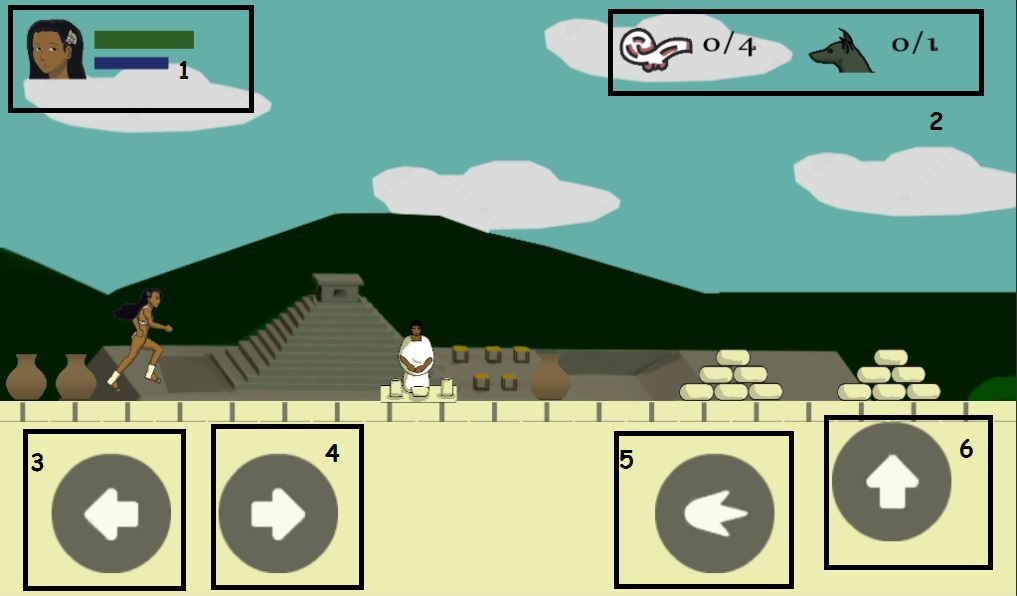
\includegraphics[height=0.3 \textheight]{Imagenes/ControlCorrerDer}
				\caption{1 Información del personaje jugable, barra verde indicador de la cantidad de vida, barra azul cantidad de tonalli. 2 Objetivos del nivel o información útil. 3 Botón moverse izquierda. 4 Botón moverse derecha. 5 Botón disparar tonalli. 6 Botón saltar.}
				\label{fig:GUI}
\end{figure}

%---------------------------------------------------------  		
    	\section{Sinopsis de contenido:} 
La historia se centra en Malinalli Tenelpan, una joven esclava que desea revivir a su padre, y el dios Xólotl, un Dios exiliado que se ha ofrecido a revivir al padre de Malinalli a cambio de su ayuda, cuyo objetivo es restaurar el orden de la jerarquía divina luego de que Tezcatlipoca y Quetzalcóatl la sumergieran en un espiral de caos con sus múltiples batallas por el liderazgo de los dioses. 
\\
\par
Para cumplir sus objetivos, Malinalli y Xólotl bajaran al Mictlan. Ahí enfrentaran a los guardianes del Mictlan, que son Dioses de gran poder cuyas habilidades se relacionan con un aspecto de la muerte. Siendo el último a vencer el señor y gobernante del Mictlan: el dios Mictlantecuhtli.
\\
\par
A lo largo de la narrativa, el jugador irá descubriendo el pasado de los dos protagonistas, de igual forma aprenderá sobre el funcionamiento del mundo de los dioses, sus reglas, su jerarquía y sus integrantes.
%---------------------------------------------------------
	\section{Categoría:}
A continuación se presentará una tabla comparativa que muestra la diferentes juegos que, por sus mecánicas o temática, pueden ser considerados como productos similares a Yolotl.
\begin{itemize}
	\item Guacamelee!!
	\begin{itemize}
		\item Microsoft Windows, OS X, Linux, PlayStation 3, PlayStation 4, PlayStation Vita, Wii U, Xbox 360, Xbox One.
		\item 103.12 a 206.03 (dependiendo de la plataforma)
		\item Plataforma, Metrodvania.
		\item Personas mayores de 10 años
		\item Diferencia: No es contexto de caracter histórico, no es móvil.
	\end{itemize}

\item Never Alone
\begin{itemize}
	\item Linux, Microsoft Windows, OS X, PlayStation 3, PlayStation 4, Wii U, Xbox One, iOS, Android.
	\item 150.00 a 89.00 (dependiendo de la plataforma)
	\item Plataforma, puzzle.
	\item Personas mayores de 10 años.
	\item Diferencia: No cuenta con estatus de vida o elementos de ataque del personaje, no es móvil.
\end{itemize}


\item Valiant Hearts
\begin{itemize}
	\item Microsoft Windows, Xbox One, PlayStation 4, PlayStation 3, wiistation 360, Android y iOS.
	\item 285.00
	\item Juego de Lógica. 
	\item Personas mayores de 13 años.
	\item Diferencia: No es un juego de plataforma, no es móvil.
\end{itemize}


\item Olympia rising.
\begin{itemize}
	\item Wii U.
	\item 95.11
	\item Acción y aventura.
	\item Mayores de 10 años.
	\item Diferencia: No es un juego móvil.
\end{itemize}


\item Jotun: Valhalla Edition.
\begin{itemize}
	\item PlayStation 4, Xbox One, Wii U, Microsoft Windows, GNU/Linux, Mac OS.
	\item 150.00
	\item Acción Aventura.
	\item Personas mayores de 13 años.
	\item Diferencia: No es un juego móvil, no es de plataforma.
\end{itemize}

\end{itemize}
%---------------------------------------------------------
	\section{Licencia:}
Atribución-NoComercial-CompartirIgual 
CC BY-NC-SA
%---------------------------------------------------------
	\section{Mecánica:}
	Haciendo uso de la pantalla touch del teléfono móvil y de una interfaz gráfica, el jugador controlará a Malinalli, siendo ella el personaje jugable durante todo el juego, salvo en un nivel en donde tanto ella como Xólotl serán los personajes jugables.   El jugador hará que Malinalli pueda moverse de izquierda a derecha, realice un salto o un salto doble, ataque con tonalli o dialogue con otros personajes.
\\
\par
En total el jugador deberá de pasar 10 niveles para terminar el juego. Cada nivel está diseñado para que el jugador tenga que superar diferentes plataformas y derrotar enemigos (enemigos comunes y jefes de nivel). Algunos niveles están más orientados a la superación de obstáculos, otros a la exploración y algunos al combate, siendo la constante entre todos (salvo el nivel introductorio), el tener que derrotar a un jefe al final del nivel.
\\
\par
La GUI contendrá cuatro botones(ver  figura \ref{fig:GUI}): uno para moverse a la izquierda, otro para moverse a la derecha, otro más para saltar y uno para disparar tonalli. En la parte superior de la pantalla habrá dos iconos uno para indicar la cantidad de vida de Malinalli y otro para la cantidad de tonalli para disparar. La cantidad de tonalli disminuirá con cada ataque que el jugador efectué y cuando éste llegué a cero, el jugador podrá disparar hasta después de que se reestablezca la barra de tonalli o si logra obtener el ítem Flor de vainilla(ver figura \ref{fig:UsoTonalli} ). Cuando un disparo de tonalli colisiona con un enemigo, éste desaparece si es un enemigo común o se le infringe una cantidad de daño determinada en caso de que sea un jefe (Ver figura \ref{fig:InterEnemigo}). La vida de Malinalli disminuirá si recibe ataques de los enemigos o si colisiona con alguno (ver figura \ref{fig:Danio}). Cada enemigo tiene una cantidad de daño asignada, siendo los jefes de cada nivel los enemigos con mayor capacidad de infringir daño. La partida acabará si la vida de Malinalli llega a cero. El jugador podrá recuperar vida con el ítem Grano de Cacao.

\begin{figure}
				\centering
				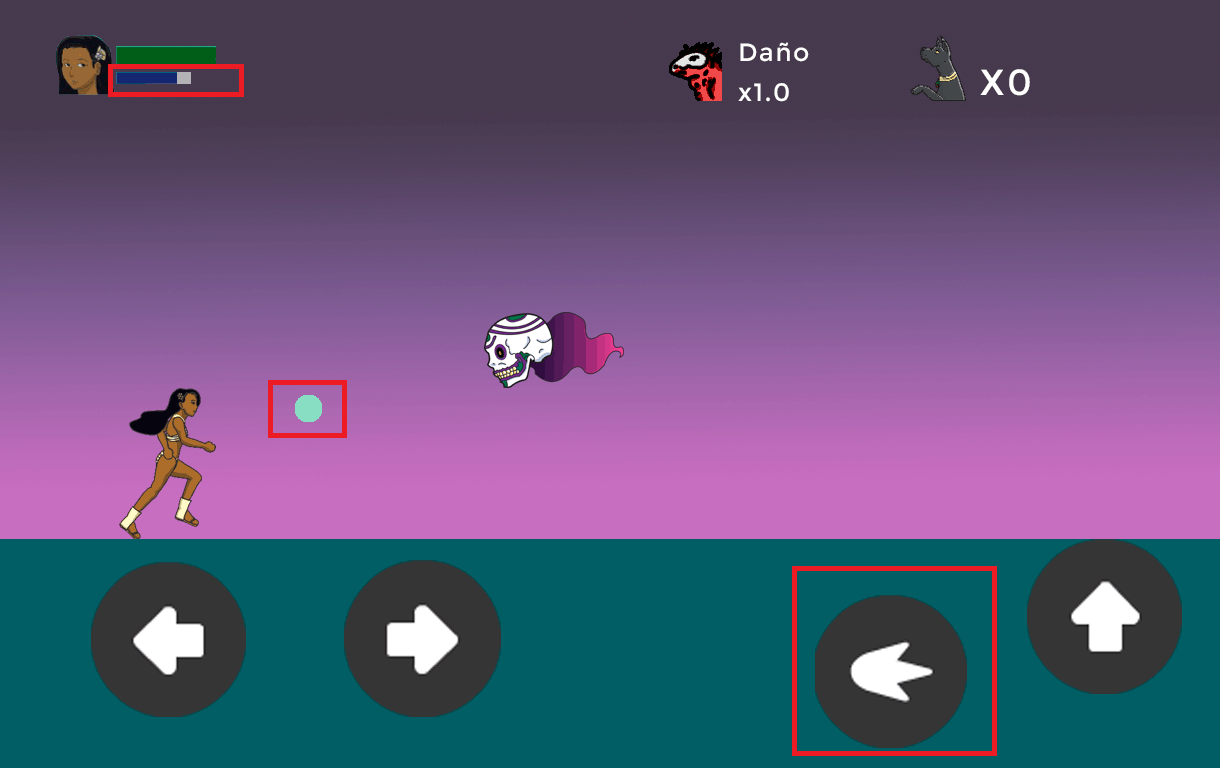
\includegraphics[height=0.3 \textheight]{Imagenes/nivel02_tonalli}
				\caption{Cuando el jugador dispara se consume una fracción de la barra de tonalli.}
				\label{fig:UsoTonalli}
\end{figure}

	\begin{figure}
  \centering
  \subfigure[Disparo de tonalli.]{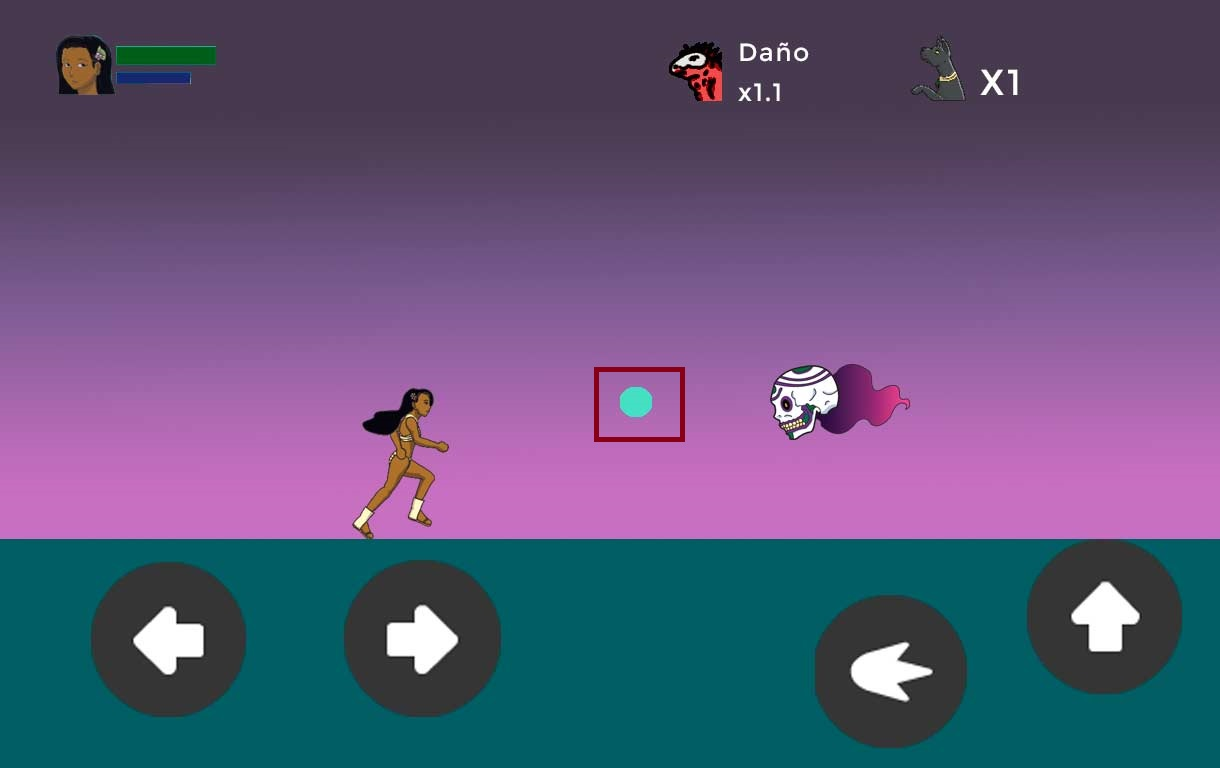
\includegraphics[width=0.45 \textwidth]{Imagenes/PantallaInteraccionEnemigo}}
   \subfigure[Colisión disparo de tonalli con enemigo común.]{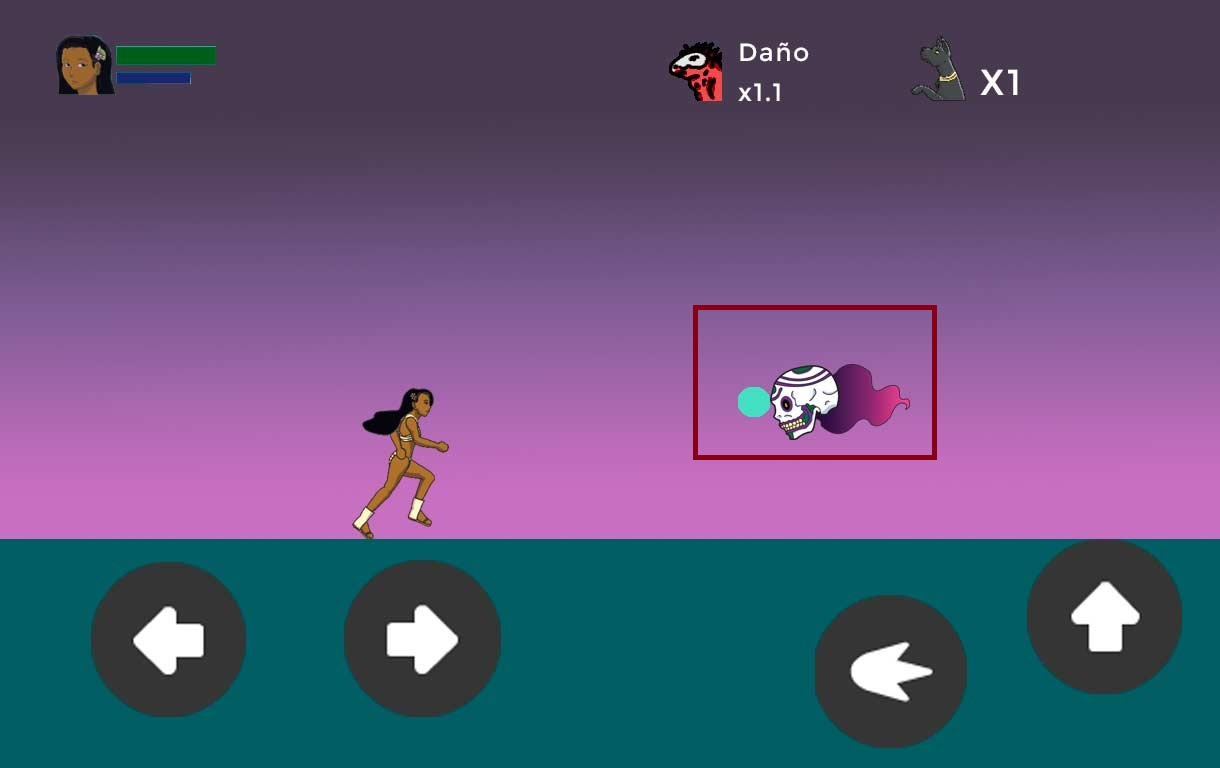
\includegraphics[width=0.3 \textwidth]{Imagenes/PantallaInteraccionEnemigo02}}
   \subfigure[Destrucción del enemigo y el disparo de tonalli.]{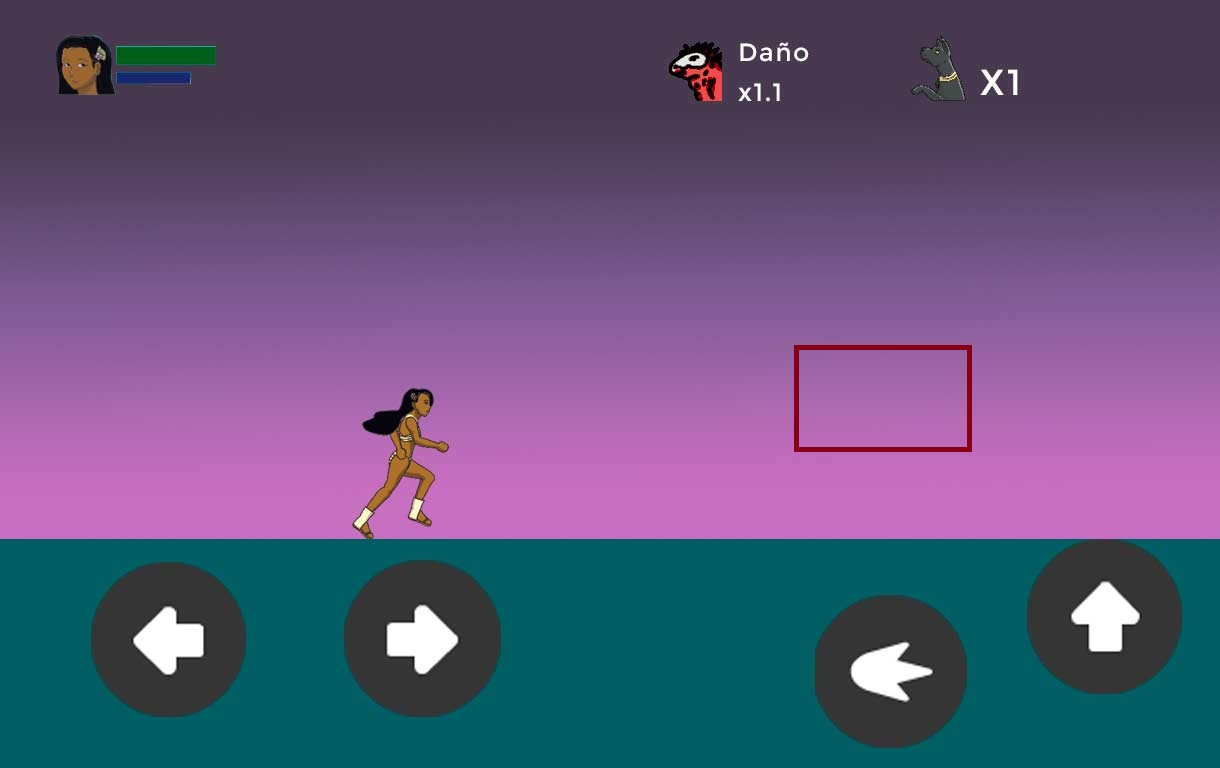
\includegraphics[width=0.3 \textwidth]{Imagenes/PantallaInteraccionEnemigo03}}
  \caption{Interacción entre el enemigo y el disparo de tonallia}
  \label{fig:InterEnemigo}
\end{figure} 

\begin{figure}
				\centering
				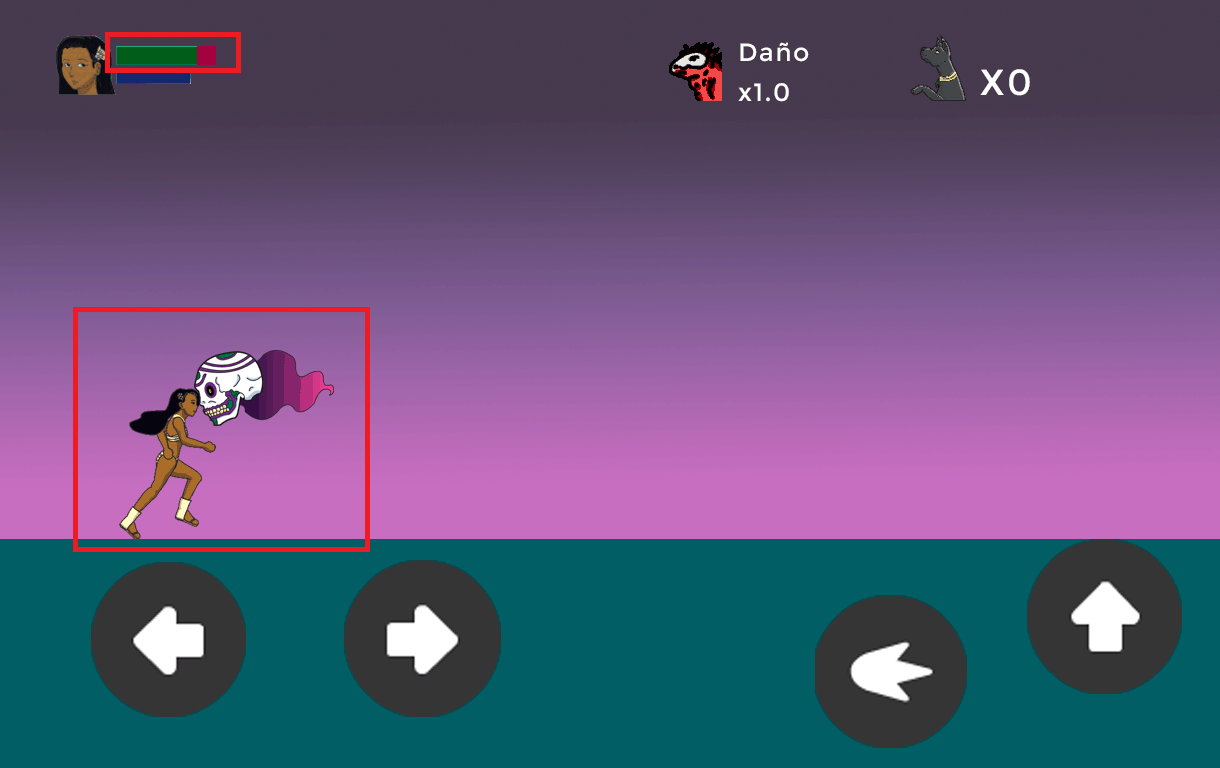
\includegraphics[height=0.3 \textheight]{Imagenes/nivel02_danio}
				\caption{Cuando el jugador colisiona con un enemigo el personaje jugable recibe daño y su cantidad de  vida disminuye, el daño recibido depende del enemigo.}
				\label{fig:Danio}
\end{figure}	%---------------------------------------------------------
	\section{Tecnología:}
\textbf{Hardware}:
\begin{itemize}
	\item Computadora DELL Inspiron 15.Procesador Intel Core i3-4005U CPU de 1.70 GHz de 64 bits. Memoria ram de 8GB.
	\item Lenovo G40. Intel Core i3 4005U CPU 1.7 Khz de 64 bits. Memoria ram de 8GB. Tarjeta gráfica AMD Radeon R5 235 de 1GB
	\item Tableta digitalizadora Intuos pen small
	\item Huawei TAG-L13. CPU de ocho núcleos a 1.5 GHZ, RAM 2GB, resolucion de 720 X 1280.
\end{itemize}
\textbf{Software}:
\begin{itemize}
	\item Sistema operativo Windows 10.
	\item Unity 3D 5.6.2.f1(64 Bits).
	\item Adobe Photoshop CS6.
	\item Corel Draw X5.
	\item TexMaker 4.5.
	\item StarUML 2.8.
	\item MiKTeX 2.9
	\item Git-2.13.3 (64 bits).
	\item Blender 2.78c.
	\item Android Studio version 2.3.3.
	\item Sistema Adroid 5.1.
	\item Unity Remote 5.
	\item Autodesk SketchBook  v3.7.6.
	
\end{itemize}	
%---------------------------------------------------------	
\section{Público:}
Jóvenes mexicanos mayores de 13 años que cuenten con un dispositivo de teléfono móvil con Android 5.1.

	%---------------------------------------------------------
\chapter{Historial de versiones}
ver.$01 26/04/2017$ Primera versión sujeta a revisión.
\\
\par
ver.$02 18/09/2017$ 
	\chapter{Visión general del juego}
Yolotl nace a partir del deseo de contar una historia con la capacidad de tocar los sentimientos del jugador, por tal motivo el juego está más orientado a la narrativa que a la jugabilidad. Sin embargo, esto no es sinónimo de que la jugabilidad no es un factor importante en el desarrollo del juego sino todo lo contrario: es otro vehículo de la narrativa permitiendo al jugador encarnar de mejor manera a los personajes al hacerlo participe de la narrativa.
\\
\par
La visión narrativa que acompaña a Yolotl es tal que su argumento combina mitología y sucesos históricos para darle una capa extra de profundidad narrativa. Permitiendo que el juego no solo sea un medio de diversión sino a su vez ofrezca una visión histórica y cultural del México prehispánico. 
\\
\par
 Una de las fortalezas de Yolotl son sus personajes, cada personaje fue cuidadosamente diseñado, prestando principal atención en los pequeños detalles que muestran los aspectos de sus personalidades. El peso que tienen los personajes sobre el juego es tal que el diseño de los niveles del Mictlán son un reflejo de su guardián, este cuidado de diseño abarca desde los enemigos comunes a enfrentar hasta la musicalización del nivel, culminando en los bloques de animación del jefe del nivel cuando se le enfrenta.
\\
\par
Desafortunadamente, esta visión narrativa del juego no es gratuita y la jugabilidad se ve afectada al ofrecer una progresión lineal al jugador, en donde cada nivel tiene objetivos muy fijos y la capacidad de exploración se ve bastante limitada. No obstante, la composición de clases de programación del juego permitirá que se puedan agregar nuevas funcionalidades sin afectar las clases y el código ya existente en un futuro.
\\
\par
Yolotl es un juego para el público que disfrute de juegos cuyo punto fuerte sea la narrativa por sobre los juego de mundo abierto. 

	\chapter{Mecánica de juego}
%=========================================================
	\section{Cámara}
El juego se manejara en 2D, desde una perspectiva lateral. La cámara será ortogonal y seguirá al jugador en sus movimientos sobre el eje x y y, existiendo algunas secciones de los niveles limites en cuanto a su desplazamiento, tal como muestra la figura \ref{fig:Camara}. 

\begin{figure}
  \centering
  \subfigure[Seguimiento horizontal]{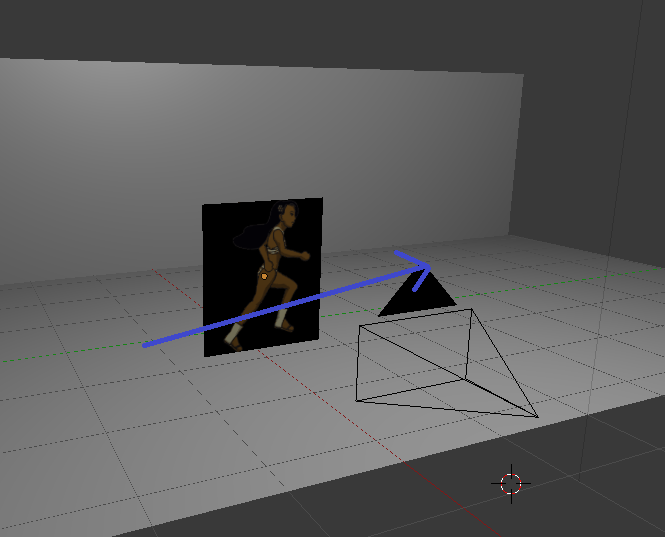
\includegraphics[width=0.7 \textwidth]{Imagenes/camara01}}
   \subfigure[Seguimiento vertical.]{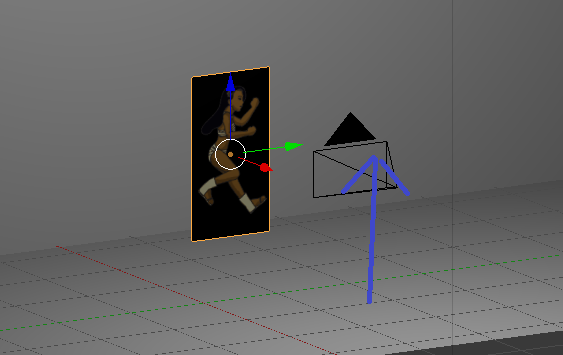
\includegraphics[width=0.7 \textwidth]{Imagenes/camara02}}
  \caption{La cámara seguirá la posición del jugador en el eje x y y.}
 %=========================================================
  \label{fig:Camara}
\end{figure} 
%=========================================================
	\section{Periféricos}
	Patalla táctil.
%=========================================================
	\section{Controles}
	Del lado izquierdo inferior de la pantalla existirán cuatro botones: dos botones de desplazamiento, uno de salto y otro de disparo.Todos estos botones son de forma circular y en conjunto ocupan un cuarto de la pantalla (ver figura \ref{fig:Controles}). A continuación se describirá cada botón y su funcionamiento.
	\begin{itemize}
		\item \textbf{Botón moverse derecha:} Botón cuyo icono es una flecha apuntando hacia la derecha. Permite al personaje jugable desplazarse hacia la derecha.
		\item \textbf{Botón moverse izquierda:} Botón cuyo icono es una flecha apuntando hacia la izquierda. Permite al personaje jugable desplazarse hacia la izquierda.
		\item \textbf{Botón disparar:} Botón cuyo icono es una flama girada noventa grados en sentido contrario de las manecillas del reloj. La acción de este botón depende de la cantidad de tonalli del personaje jugable. Cuando ésta es mayor a cero, el jugador dispara esferas de energía que desaparecen después de determinado tiempo. Estas esferas de energía pueden efectuar una cantidad de daño en los enemigos de cada nivel pero no tienen efecto sobre los obstáculos. Cada disparo decrementa la cantidad de tonalli total de manera constante, cuando ésta llega a cero el jugador no podrá realizar ningún disparo hasta que se recargue la barra de cantidad de tonalli(la cual tiene un tiempo de recarga automática una vez que llega a cero) o toque el item de flor de vainilla.
		\item \textbf{Botón saltar:} El icono de este botón es una flecha que apunta hacia arriba. Este botón solamente se puede accionar dos veces seguidas, es decir permite hacer de manera consecutiva dos saltos.  
	\end{itemize}
	\begin{figure}
  \centering
  \subfigure[Acción del botón de moverse derecha.]{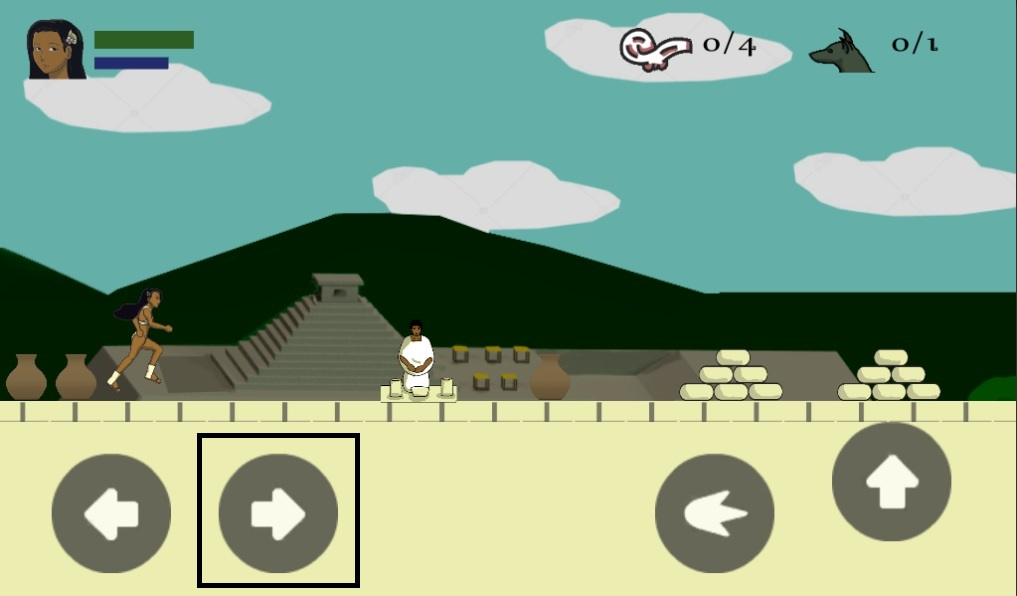
\includegraphics[width=0.45 \textwidth]{Imagenes/ControlCorrerDerGUI}}
   \subfigure[Acción del botón de moverse izquierda.]{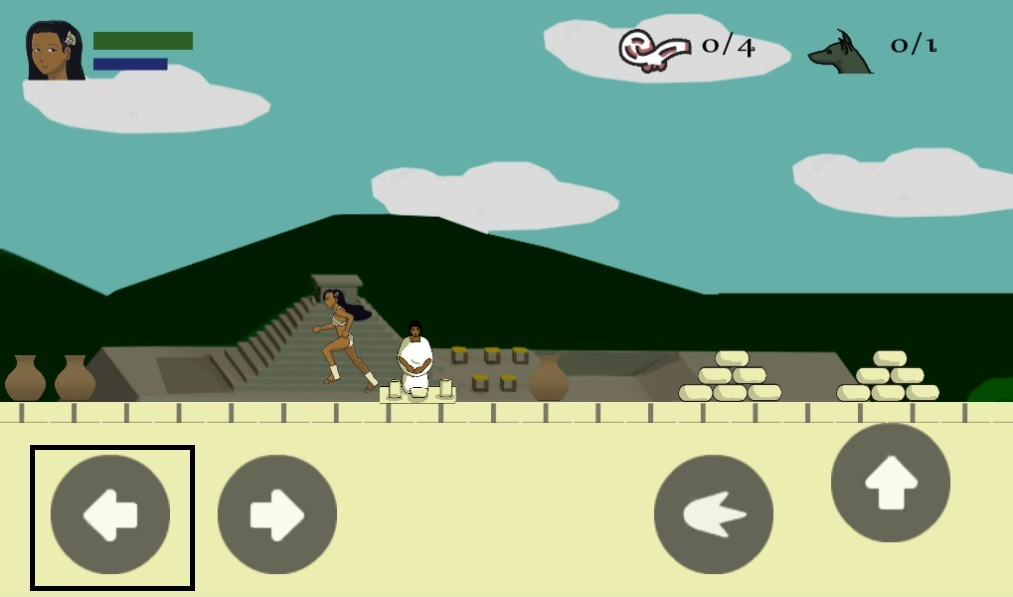
\includegraphics[width=0.45 \textwidth]{Imagenes/ControlCorrerIzq}}
   \subfigure[Acción del botón de disparar.]{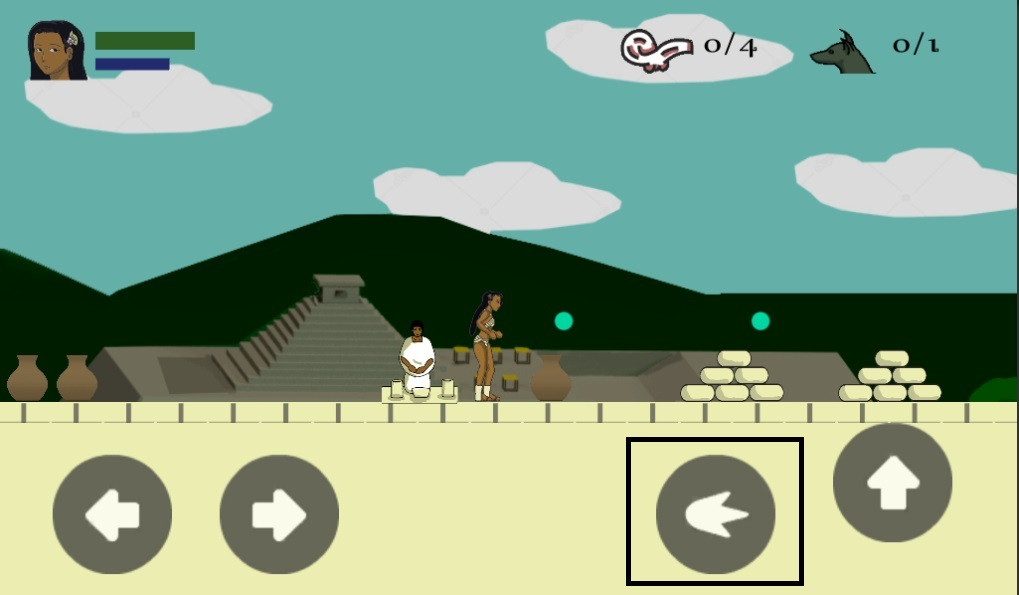
\includegraphics[width=0.45 \textwidth]{Imagenes/Controldispara}}
   \subfigure[Acción del botón de saltar.]{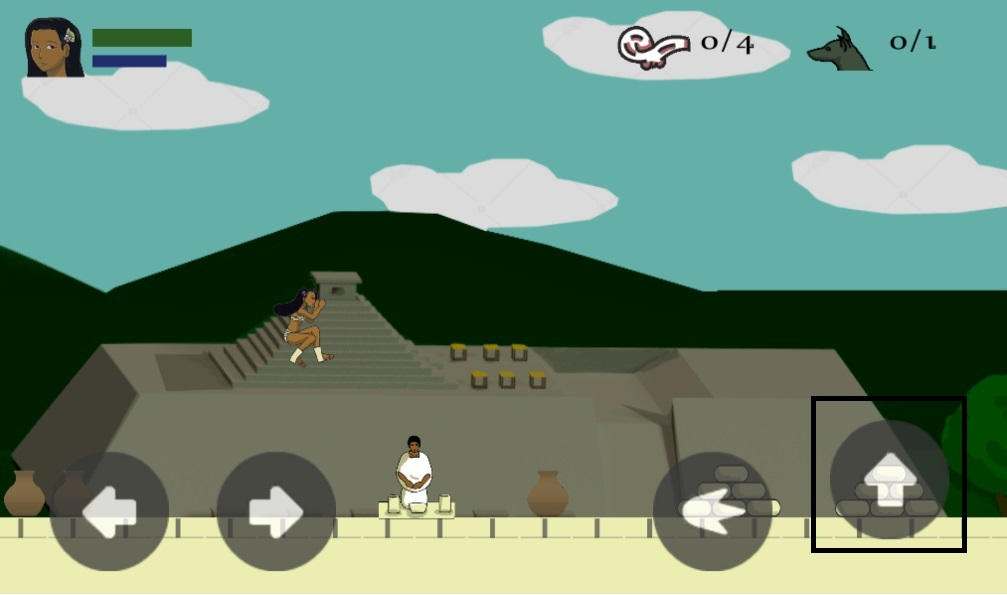
\includegraphics[width=0.45 \textwidth]{Imagenes/ControlSalta}}
  \caption{Acciones que desencadena cada botón.}
  \label{fig:Controles}
\end{figure} 
%=========================================================
	\section{Guardar/Cargar}
	%---------------------------------------------------------
\subsection{Guardar}
Dentro del juego existen dos tipos de guardado en el juego: el guardado automático y el checkpoint. 
\begin{itemize}
\item \textbf{Guardado automático}: 
Este tipo de guardado se realizará cuando el jugador haya completado un nivel. En este tipo de guardado se almacenara información como los niveles y cinemáticas disponibles, y las estadísticas del jugador(cantidad de vida, cantidad de tonalli y capacidad de daño). 
\item \textbf{Checkpoint}: 
Este tipo de guardado almacena la posición del jugador en un punto determinado del nivel. Los puntos de checkpoint son representados dentro del juego con el objeto Tecolote. El checkpoint se activará cuando el jugador colisione con el objeto tecolote( ver apartado \ref{per:tecolote}) . Este tipo de guardado es efectivo mientras el jugador se mantenga dentro del nivel y la información almacenada se perderá si el jugador abandona la partida.
Los puntos de checkpoint están disponibles a partir del segundo nivel del juego y hasta el noveno nivel. La cantidad de checkpoints dependerá del nivel, pudiendo haber de dos a cuatro checkpoints. 
\end{itemize}
%---------------------------------------------------------
\subsection{Cargar}
Dentro del juego existen dos tipos de carga en el juego: carga automática y el checkpoint. 
\begin{itemize}
\item \textbf{Carga automática}: 
Este tipo de cargado se realizará cuando el jugador seleccione la opción de cargar partida desde la Interfaz 2.00(ver apartado \ref{inter:interfaz02})o cuando el jugador se encuentre en la interfaz 03 (ver apartado \ref{inter:interfaz03}). En este tipo de carga le permite al juego conocer el progreso del jugador, por lo que en esta carga el juego conocerá información como los niveles y cinemáticas disponibles, y las estadísticas del jugador (cantidad de vida, cantidad de tonalli y capacidad de daño). 
\item \textbf{Checkpoint}: 
Este tipo de carga permite que el jugador pueda aparecer en la posición del ultimo objeto Tecolote ( ver apartado \ref{per:tecolote}) con el que se haya colisionado dentro del juego una vez que el jugador haya muerto y no haya abandonado la partida. Cuando se carga la posición del jugador en el Checkpoint, el jugador recuperara al máximo la cantidad de vida y de tonalli que tenga disponible para ese nivel.
\end{itemize}
			

	\chapter{Estados del juego}
Sin contar los niveles y las cinemáticas, el juego se compone de tres interfaces: Interfaz 1.00 (Ver interfaz \ref{inter:interfaz01}), correspondiente a la pantalla de inicio; la interfaz 2.00 (Ver interfaz \ref{inter:interfaz02}), que corresponde al menú principal; y la interza 3.00 (Ver interfaz \ref{inter:interfaz03}), correspondiente al menu de selección de nivel. Como se puede ver en la figura %%\ref{}  

Ver figura \ref{fig:EstadosJuego}
\begin{figure}
  \centering
     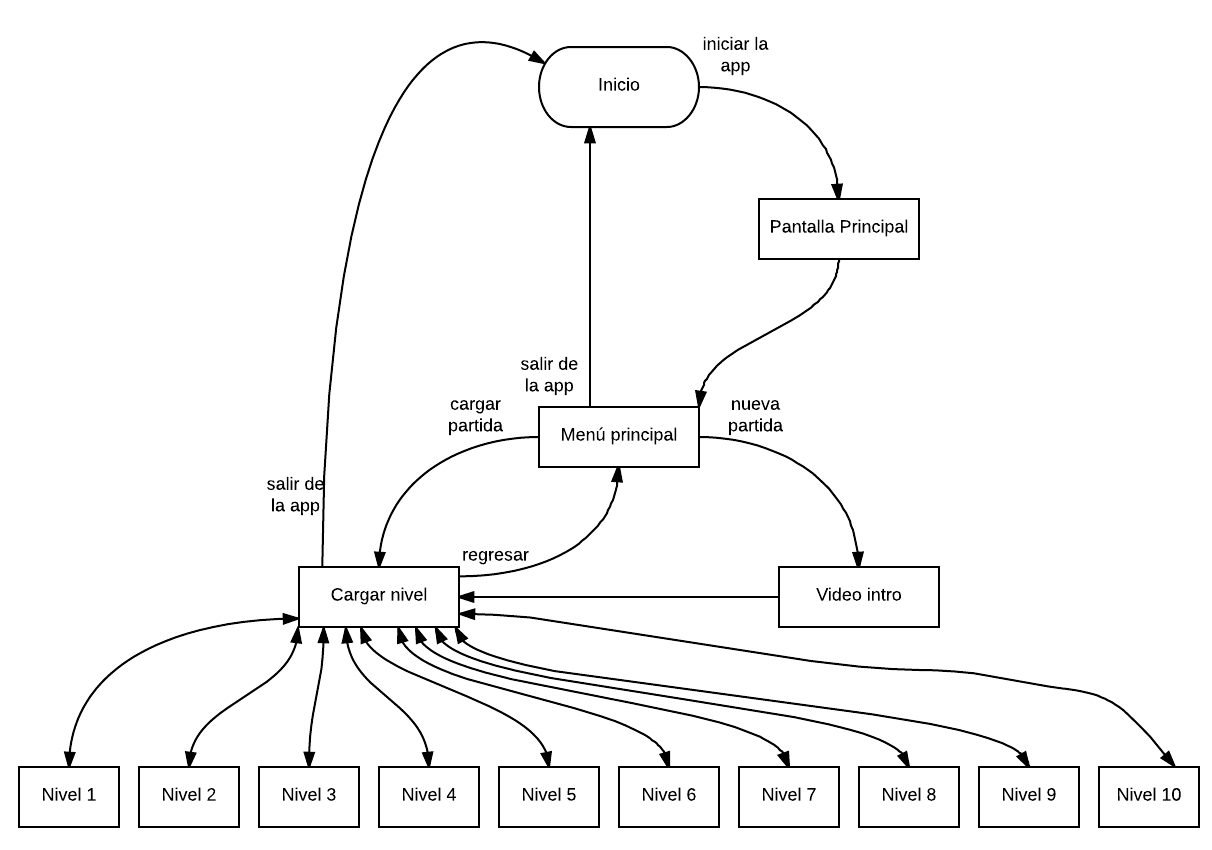
\includegraphics[width=\linewidth]{Imagenes/estadosJuego}
  \caption{Progreso del juego}
  \label{fig:EstadosJuego}
\end{figure} 
	\chapter{Interfaces}
		\subsubsection{Interfaz 1.00 Pantalla de inicio.} \label{inter:interfaz01}
	\subsubsection{Descripción de la pantalla}
Todos los elementos se encuentran centrados en esta pantalla. En la parte centro superior se encuentra el logotipo del juego. Abajo de éste, se puede leer el mensaje: "Toque la pantalla para empezar". Al pie de la pantalla se puede ubica la información de derechos de autor del juego.
	\subsubsection{Estados del juego}
Es el estado inicial del juego.
Al tocar la pantalla se muestra la Interfaz 2.0 (ver apartado \ref{inter:interfaz02}).
	\subsubsection{Imagen}
\begin{figure}
  \centering
   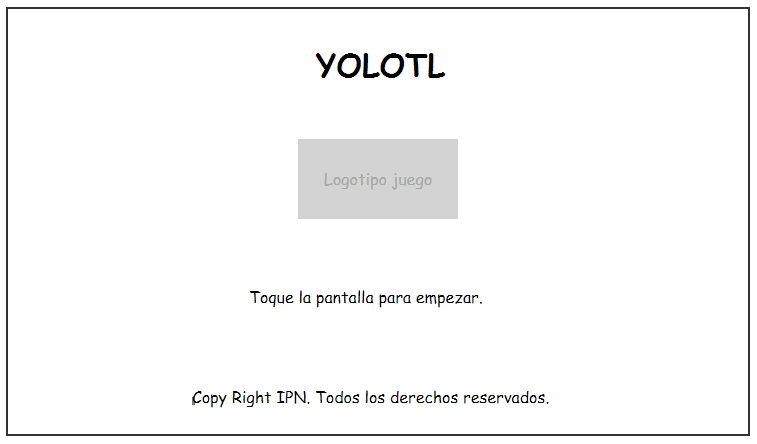
\includegraphics[width=0.6 \textwidth]{05TrabajoRealizado/01DocDiseno/Interfaz/imagenes/interfaz00}
  \caption{Interfaz 1.0 Pantalla de inicio.}
  \label{fig:PInicio}
\end{figure} 

Ver figura \ref{fig:PInicio}

	\subsubsection{Interfaz 2.00 Menú principal.} \label{inter:interfaz02}
	\subsubsection{Descripción de la pantalla}
El logotipo del juego se muestra en la parte superior derecha de la pantalla. En la parte inferior izquierda se muestran las dos opciones: Nueva partida, Cargar partida. De fondo se muestra la misma Imagen que en la interfaz 01.00. 
Cada opción desencadena un cuadro de dialogo en donde el usuario debe de confirmar la acción que va desea ejecutar o en donde se le informa que la acción seleccionada no es posible de ejecutar.
	\subsubsection{Estados del juego}
La interfaz 2.00 contiene los siguientes botones:
\begin{itemize}
	\item \textbf{Nueva partida}:  Dirige a la presentación de la cinemática 1 (ver apartado \ref{Cin:Cinematica01}).
	\item \textbf{Cargar partida}: Dirige a la interfaz 3.00 (ver apartado \ref{inter:interfaz03}) en caso de que exista una partida previamente guardada, en caso contrario abre un cuadro de dialogo en donde se le dice al Jugador que no existe partidas que cargar.
\end{itemize}
Se puede llegar a esta Interfaz a partir de la Interfaz 01.00 (ver apartado \ref{inter:interfaz01})
	\subsubsection{Imagen}
Ver figura \ref{fig:PMenuP}
\begin{figure}
  \centering
   \subfigure[Menú principal] {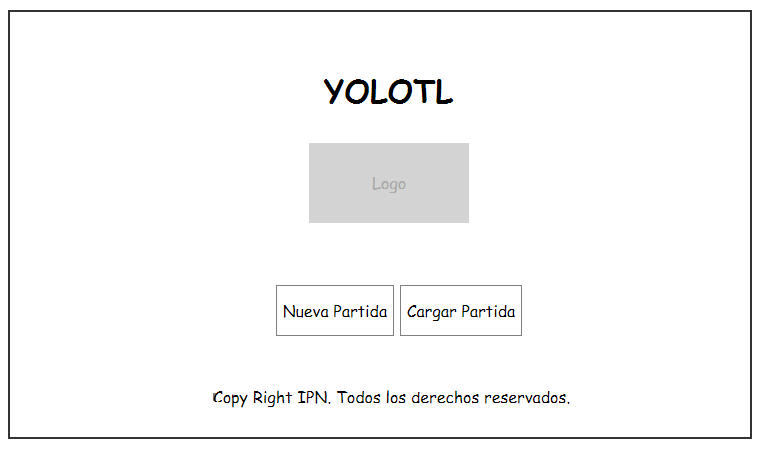
\includegraphics[width=0.6 \textwidth]{05TrabajoRealizado/01DocDiseno/Interfaz/imagenes/interfaz01}}
   
 	\subfigure[Cuadro de dialogo para confirmar iniciar nueva partida.] {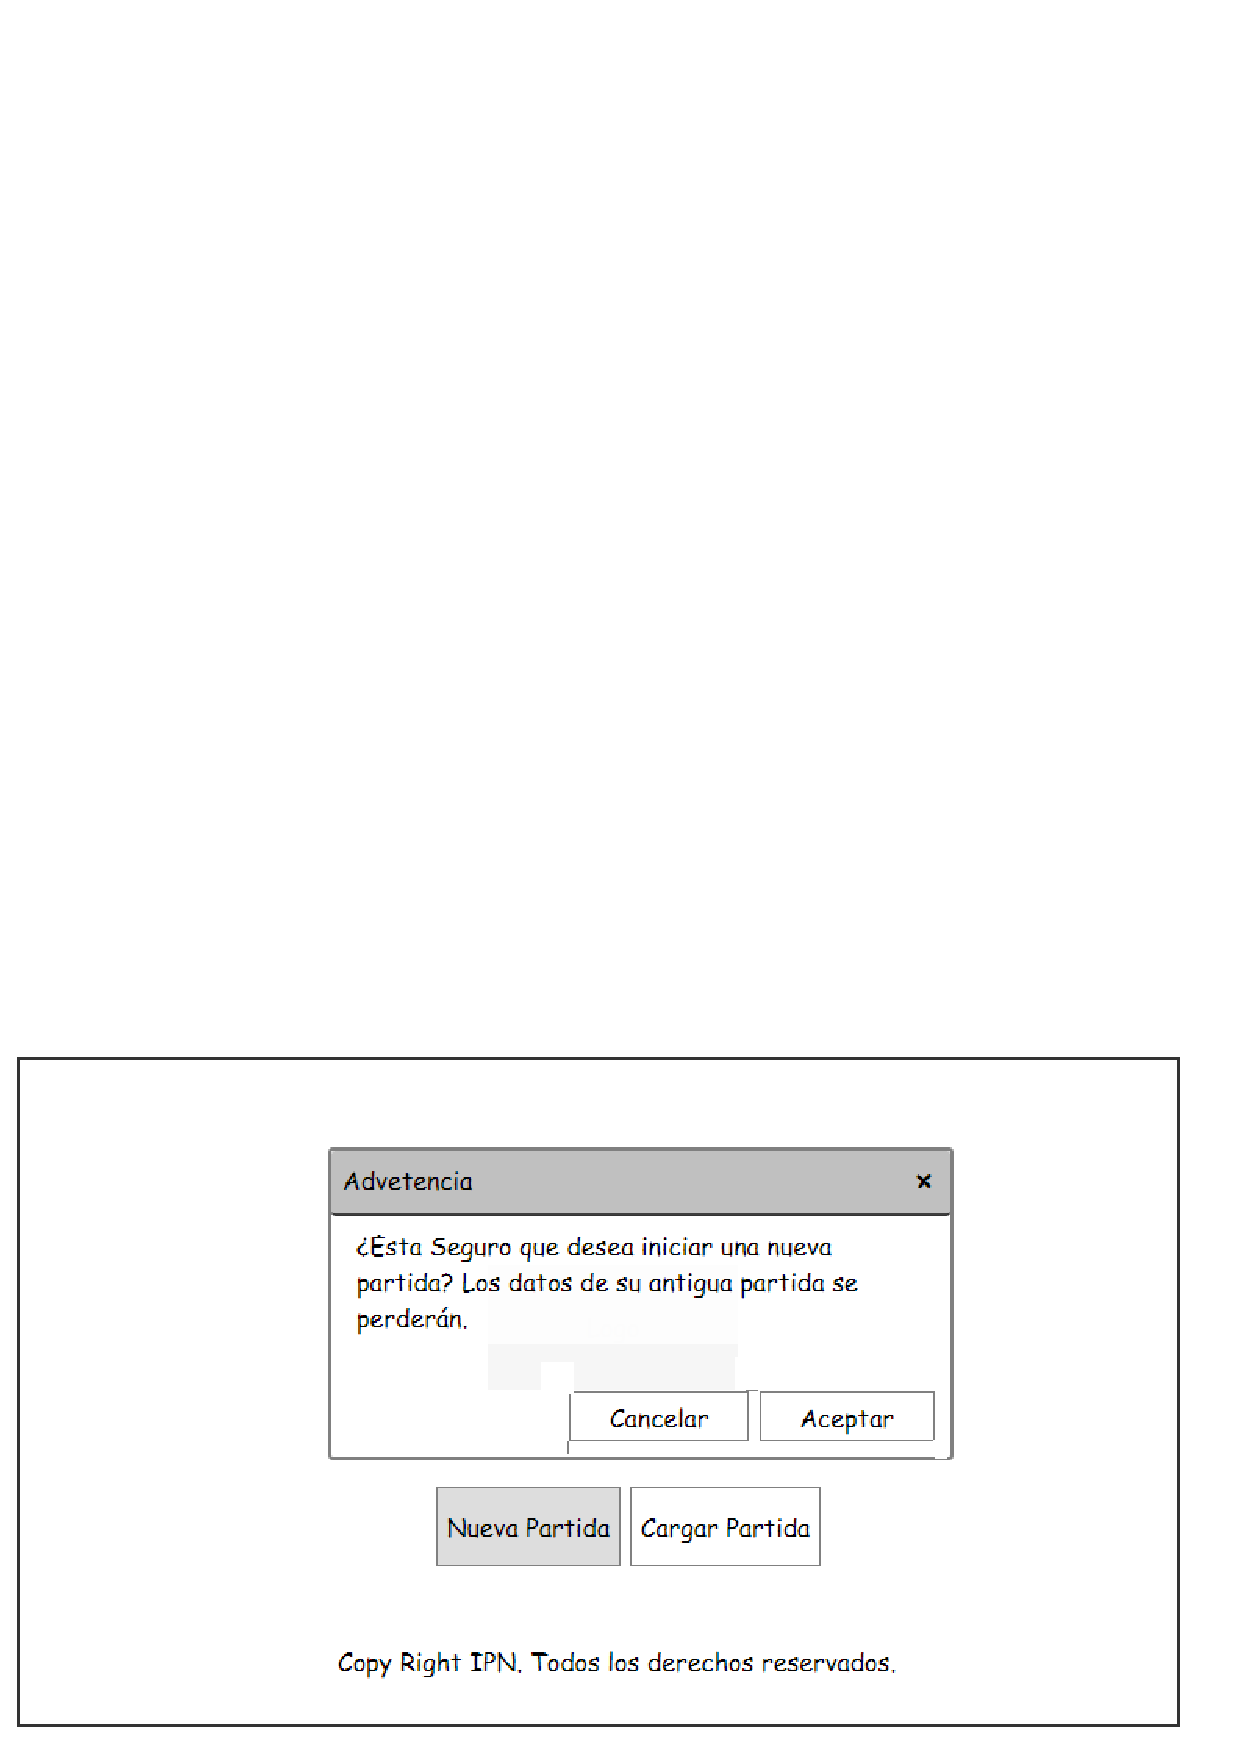
\includegraphics[width=0.6 \textwidth]{05TrabajoRealizado/01DocDiseno/Interfaz/imagenes/interfaz01_02}}
 	
\subfigure[Cuadro de dialogo cuando no existen partidas que cargar.] {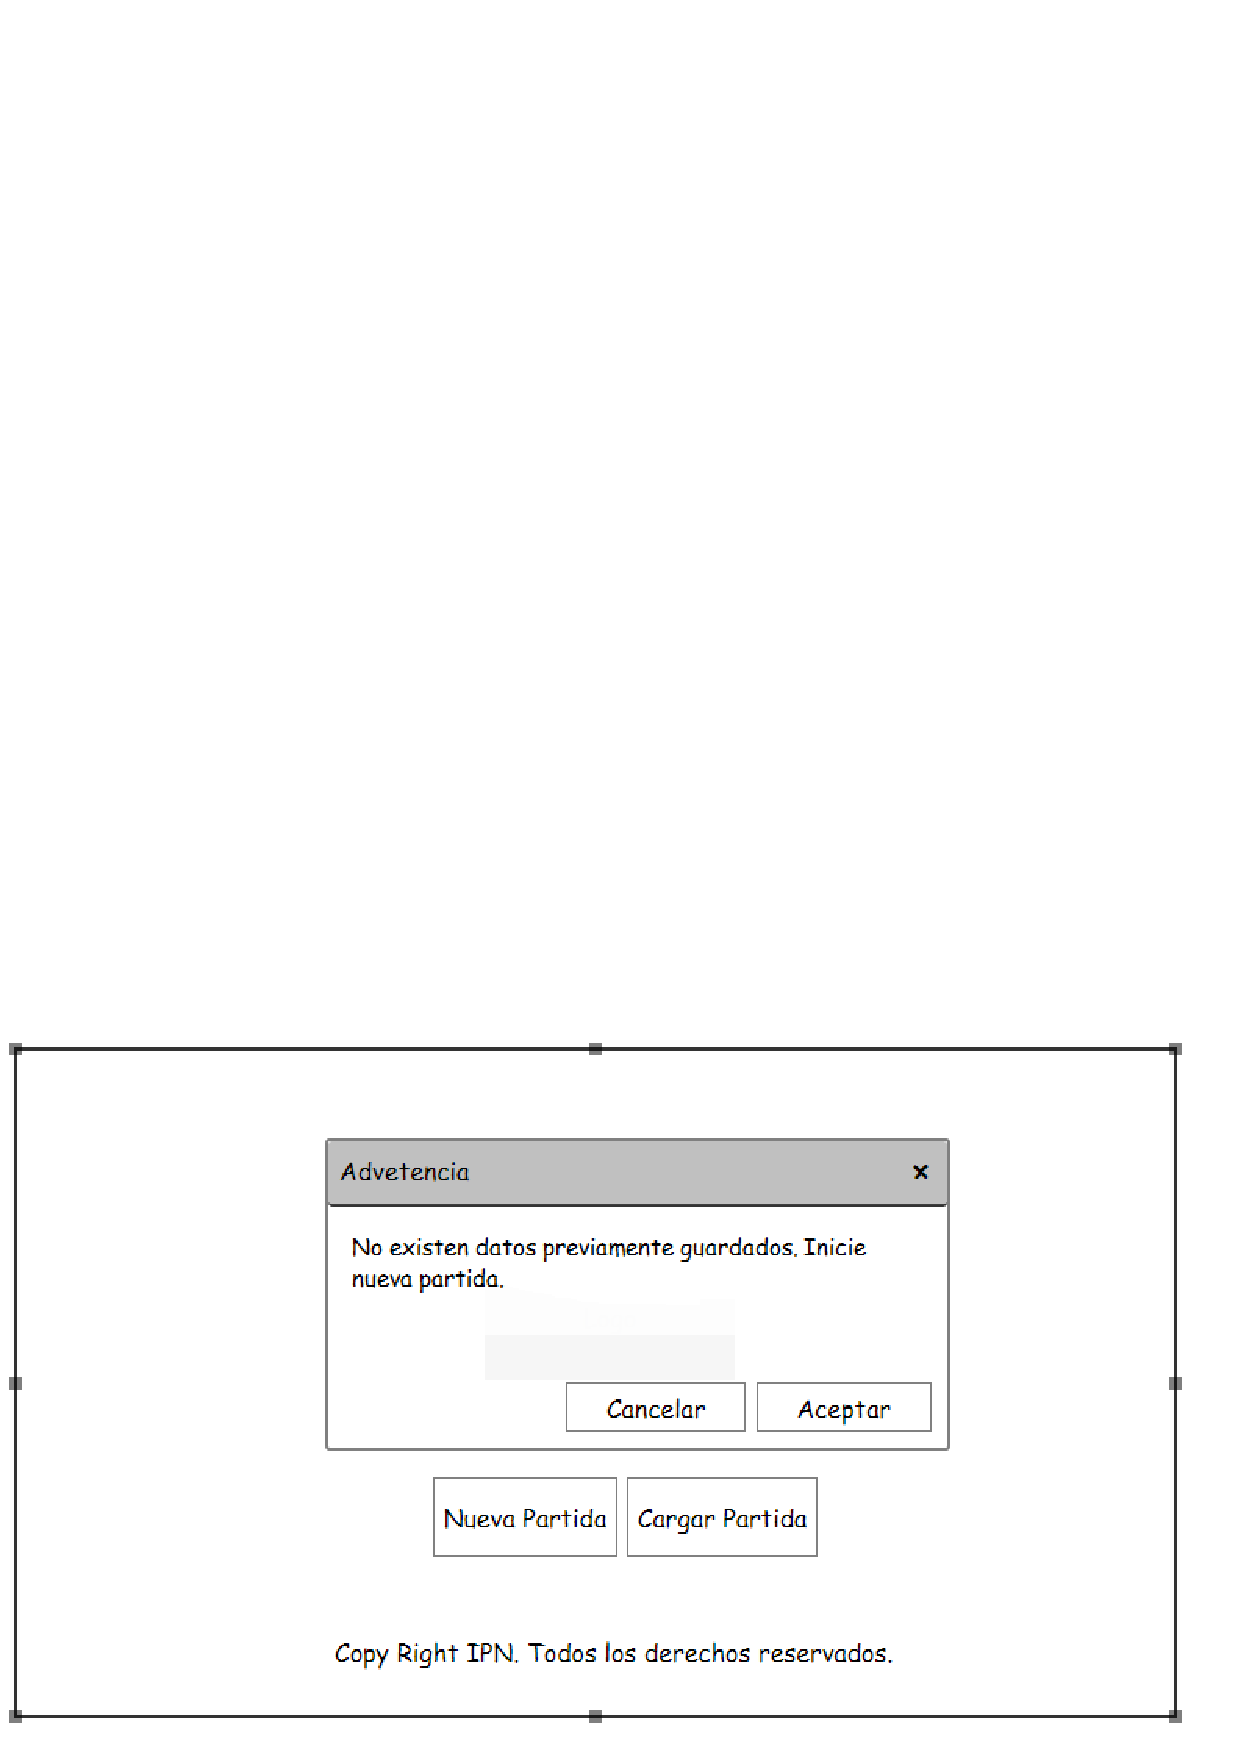
\includegraphics[width=0.6 \textwidth]{05TrabajoRealizado/01DocDiseno/Interfaz/imagenes/interfaz01_03}}
  \caption{Interfaz 2.00 Menú principal.}
  \label{fig:PMenuP}
\end{figure} 
	\section{Interfaz 3.00 Selección de nivel}\label{inter:interfaz03}
	\subsection{Descripción de la pantalla}
Muestra el nombre de la pantalla en la esquina superior izquierda.
Los iconos de nivel y de las cinemáticas estarán organizados en un carrusel que permitirá su selección. Los niveles y cinemáticas disponibles a elegir en el carrusel dependerán de la carga automática. Los niveles disponibles disponibles para jugar mostrarán una imagen descriptiva en el carrusel mientras que los niveles no disponibles mostraran un imagen de un cuadro negro.   
Bajo el carrusel se encontrara un apartado donde se podrá visualizar información del nivel seleccionado en el carrusel, tal como el nombre y una breve descripción.
El botón que permite iniciar una partida en el nivel seleccionado se encontrará ubicado al lado derecho de la sección donde se muestra la información del nivel. 
	\subsection{Estados del juego}
Se llega a esta interfaz a través de la interfaz 2.00 (ver apartado\ref{inter:interfaz02}), siempre que el Jugador oprima el botón de cargar partida.
La interfaz 3.0 cuenta con los siguientes botones:
\begin{itemize}
	\item \textbf{Iniciar Nivel}: Envía al inicio del nivel seleccionado.
	\item \textbf{Control de carrusel}: estos botones permite controlas los elementos que se almacenan en el carrusel.
\end{itemize} 
	\subsection{Imagen}
	Ver figura \ref{fig:SelNivel}
\begin{figure}
  \centering
   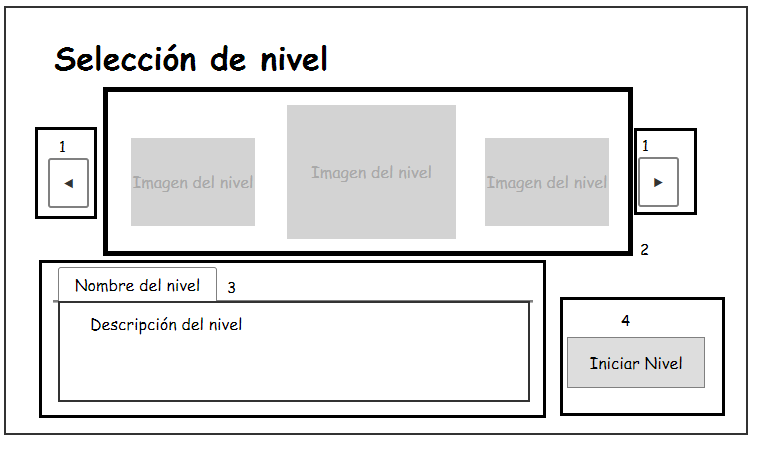
\includegraphics[width=0.6 \textwidth]{Imagenes/interfaz02_01}
  \caption{Interfaz 2.00 Selección de nivel.1 botones que controlan el carrusel. 2 Carrusel. 3 Información del nivel seleccionado. 4 Botón Iniciar nivel.}
  \label{fig:SelNivel}
\end{figure} 
		\chapter{Niveles}
		\section{Nivel 1} \label{Nivel:Intro}
	\subsection{Título del nivel}
	La chica y el perro.
	\subsection{Encuentro}
Nivel introductorio que le permite al jugador familiarizarse con las mecánicas básicas de juego: saltar, moverse y abrir y cerrar cuadros de dialogo. Además, este nivel servirá para mostrar el contexto histórico en el que se sitúa el argumento del juego.
	\subsection{Descripción}
	Este nivel se divide en dos etapas: la etapa Tianguis y la etapa selva. A continuación se describirá en que consiste cada etapa.
	\begin{itemize}
		\item\textbf{Tianguis}: El jugador controlará a Malinalli y recorrerá un mercado, en donde podrá dialogar con diferentes ciudadanos (ver apartado \ref{per:ciudadanos}). Una vez terminada la interacción con los ciudadanos el jugador tendra disponible la opción de
dialogar con Xólotl, lo que activará la cinemática 2 (ver apartado \ref{Cin:Cinematica02}).		
		\item\textbf{Selva}: El jugador tendrá que perseguir a Xólotl por la selva para recuperar el objeto que éste le robó durante la cinemática 2 (ver apartado \ref{Cin:Cinematica02}).  Xólotl utiliza este encuentro para probar la valentía de Malinalli ante situaciones en las que se encuentre en peligro, pero sin la oportunidad de defenderse.    
		
	\end{itemize}

	\subsection{Objetivos}
\begin{itemize}
	\item \textbf{Tianguis}:
	\begin{itemize}
		\item El jugador deberá de activar al menos cuatro diálogos para poder desbloquear la infección con Xólotl, lo que mostrará la cinemática 2 (ver apartado\ref{Cin:Cinematica02}).	
		\item El jugador solo podrá dialogar con aquellos ciudadanos que posean el icono de dialogo sobre ellos. La interacción entre Malinalli y los ciudadanos se dará cuando el jugador colisione con un ciudadano que posea un icono de dialogo y pulse el botón de disparo, esta acción hará que aparezca un cuadro de dialogo; la interacción entre el jugador y el ciudadano terminara cuando el jugador pulse el botón de disparo para cerrar el cuadro de dialogo. El contador  que le permite al jugador conocer cuantos diálogos han sido activados debido a la interacción con ciudadanos, se encontrará en la parte superior derecha de la pantalla. Este contador estará precedido del icono de dialogo. Seguido de este contador habrá otro contador precedido por un icono con la imagen de Xólotl, esto con el fin de ayudarle al jugador a saber que tendrá que interactuar con Xólotl en ese nivel. El contador de diálogos se actualizará solamente cuando se intercatue por primera vez con un ciudadano, por lo que no será posible que el juego contabilice dos veces una interacción con el mismo ciudadano. 
		\item El jugador interactuará con Xólotl del mismo modo que con los ciudadanos, con la diferencia que en lugar de que aparezca un cuadro de dialogo de esta interacción, se desencadenará la cinemática 2 (ver apartado \ref{Cin:Cinematica02}) y se cargará la zona de selva.
	\end{itemize}
				
	\item \textbf{Selva}: 
		\begin{itemize}
			\item 	El jugador deberá de seguir a Xólotl. Durante la persecución deberá de superar obstáculos y plataformas saltándolos. Durante la persecución Xólotl siempre mantendrá una distancia fija del jugador, haciéndolo imposible de atrapar. El objetivo de hacer imposible de atrapar a Xólotl es garantizar que el jugador llegue a la zona en donde se desarrollara la cinemática 3  (ver apartado \ref{Cin:Cinematica03}).
			\item Obtener la caracola (ver apartado \ref{Arma:Caracola}).
			\item Ver cinemática 3 (ver apartado \ref{Cin:Cinematica03}).
	\end{itemize}
\end{itemize}
	\subsection{Progreso}
	Al concluir el nivel el jugador:
\begin{itemize}
	\item El jugador podrá ver las siguientes cinemáticas:
	\begin{itemize}
		\item Cinemática 3 (ver apartado \ref{Cin:Cinematica03}).
		\item Cinemática 4 (ver apartado \ref{Cin:Cinematica04}).
	\end{itemize}
\item Desbloqueará el segundo nivel del juego (ver apartado \ref{Nivel:Niv02}) en el menú de selección de nivel (ver apartado \ref{inter:interfaz03}).
\item Obtendrá el objeto caracola con lo que se habilitará el botón de disparo en la interfaz gráfica del juego.
\end{itemize}
	\subsection{Enemigos}
Al ser un nivel introductorio de mecánicas de juego no orientadas al combate, el nivel no cuenta con enemigos.
	\subsection{Items}
Ningún item utilizable.
	\subsection{Personajes}
\begin{itemize}
\item Malinalli (ver apartado\ref{per:malinalli}).
	\begin{itemize}
		\item Animación correr.
		\item Animación saltar. 
		\item Animación normal. 
	\end{itemize}	
\item Xólotl (ver apartado \ref{per:xolotl}).
	\begin{itemize}
		\item Xoloitzcuintle.
			\begin{itemize}
				\item Animación correr.
				\item Animación normal. 
		\end{itemize}	
		\item Jaguar.
			\begin{itemize}
				\item Animación correr.
				\item Animación normal. 
		\end{itemize}	
	\end{itemize}	

\item Ciudadanos (ver apartado \ref{per:ciudadanos}).
	\begin{itemize}
		\item Mujer comerciante. 
			\begin{itemize}
				\item Animación mover mercancía de un lado a otro.
			\end{itemize}
		\item Mujer jarrón.
			\begin{itemize}
				\item Animación caminar.
			\end{itemize}			 
		\item Hombre jarrón.
			\begin{itemize}
				\item Animación caminar.
			\end{itemize} 
		\item Hombre cacao.
			\begin{itemize}
				\item Animación caminar.
			\end{itemize}
		\item Hombre noble.
			\begin{itemize}
				\item Animación revisar mercancía(Si esta cerca de un puesto). 
				\item Animación platicar (Si esta cerca de otro noble).
				\item Animación contar granos de cacao (Si no esta cerca de un puesto o de un noble).
			\end{itemize}				
	\end{itemize}	 
\end{itemize}
\subsection{Escenario}
\begin{itemize} 
	\item Fondo:
\begin{itemize}
			\item Ciudad de \ref{Centla}: Se ve el templo a la lejanía y unas casas. Este fondo se usará en la etapa del tianguis del nivel.
			\item Selva: La ciudad se ve más alejada, hay árboles en un plano más cercano. Este fondo se utilizará en la etapa de la selva  
\end{itemize}	
	\item Suelo:
		\begin{itemize}
			\item Suelo pavimentado: Será usado en el tianguis.
			\item Suelo con pasto: Será usado en la selva.
		\end{itemize}
	\item Obstáculos:
		\begin{itemize}
			\item Tianguis
				Sin obstáculos.
			\item Selva
				\begin{itemize}
					\item Caja. Ver en \ref{obs.caja}.
					\item Sacos Cacao. Ver en \ref{obs.saco}.
				\end{itemize}
		\end{itemize}
	\item Objetos de fondo:
		\begin{itemize}
			\item Tianguis
				\begin{itemize}
					\item Jarrón
					\item Saco de cacao
					\item Sacos de cacao apilados
				\end{itemize}
			\item Selva
				\begin{itemize}
					\item Arbusto
				\end{itemize}

		\end{itemize}
\end{itemize}	
\subsection{Referencia a BGM y SFX}
\begin{itemize} 
	\item BGM.
	\begin{itemize}
		\item Música  mercado (ver apartado \ref{Musica:N01_ZN01}).
		\item Música  selva (ver apartado \ref{Musica:N01_ZN02}).
		\item Música  Xolotl (ver apartado \ref{Musica:Xolotl}).
	\end{itemize} 
	\item SFX:
	\begin{itemize}
		\item Bullicio (ver apartado \ref{SFX:Bullicio}).
		\item Pasos (ver apartado \ref{SFX:Pasos}).
		\item Viento (ver apartado \ref{SFX:Viento}).
		\item Ladrido (ver apartado \ref{SFX:Ladrido}).
\	end{itemize}
\end{itemize}
\subsection{Referencia a FX}
\begin{itemize}
	\item Circulo de luz (ver apartado \ref{FX:CirLuz}).
\end{itemize}
\end{itemize}
		\section{Nivel 2} \label{Nivel:Niv02}
	\subsection{Título del nivel}
	Nadie cruza mis dominios.
	\subsection{Encuentro}
El nivel le enseñara al jugador las mecánicas de combate: combate simple contra enemigos y el combate contra un jefe. Este nivel estará disponible después de terminar el primer nivel (ver apartado \ref{Nivel:Niv01}).
	\subsection{Descripción}
Malinalli y Xólotl se adentran al inframundo. Su primer reto a superar será cruzar el río de Apanohuaia y sus peligros para poder derrotar al primer guardián del inframundo: la iguana gigante Xochitonal. Xólotl adopta la forma de un ajolote de gran tamaño para que ambos puedan cruzar el río, por lo que el jugador controlara al Sprite de Malinalli sobre un ajolote de gran tamaño. 
	\subsection{Objetivos}
\begin{itemize}
	\item Aprender a utilizar el funcionamiento de los ataques de Malinalli y de los ítems flor de vainilla (ver apartado \ref{item:vainilla}) y grano de cacao (ver apartado \ref{item:cacao}).
	\item El jugador deberá de atravesar el lago derrotando a los enemigos que encuentre en el camino. Para derrotar a los enemigos el jugador disparará tonalli.
	\item El jugador deberá evitar tocar los Xoloitzcuintles que hay en todo el nivel ya que la capacidad de infringir daño de Xochitonal estara ligada a la cantidad de Xoloitzcuintles tocados por el jugador. Una vez que el jugador hace contacto con un Xoloitzcuintle, el Xoloitzcuintle desaparecerá y se incrementará en uno el indicador de la cantidad de Xoloitzcuintles tocados y el indicador de la cantidad de daño que puede efectuar Xochitonal (Ver figura \ref{fig:InterNivel2}). Los indicadores de la cantidad en la que se incrementa el daño que puede infringir Xochitonal y el numero de Xoloitzcuintles tocados se mostraran en la parte superior derecha de la pantalla (Ver figura \ref{fig:GUICtrlNivel2}).
	\item El jugador deberá vencer al guardián del primer nivel del inframundo, Xochitonal.
\end{itemize}

\begin{figure}
  \centering
   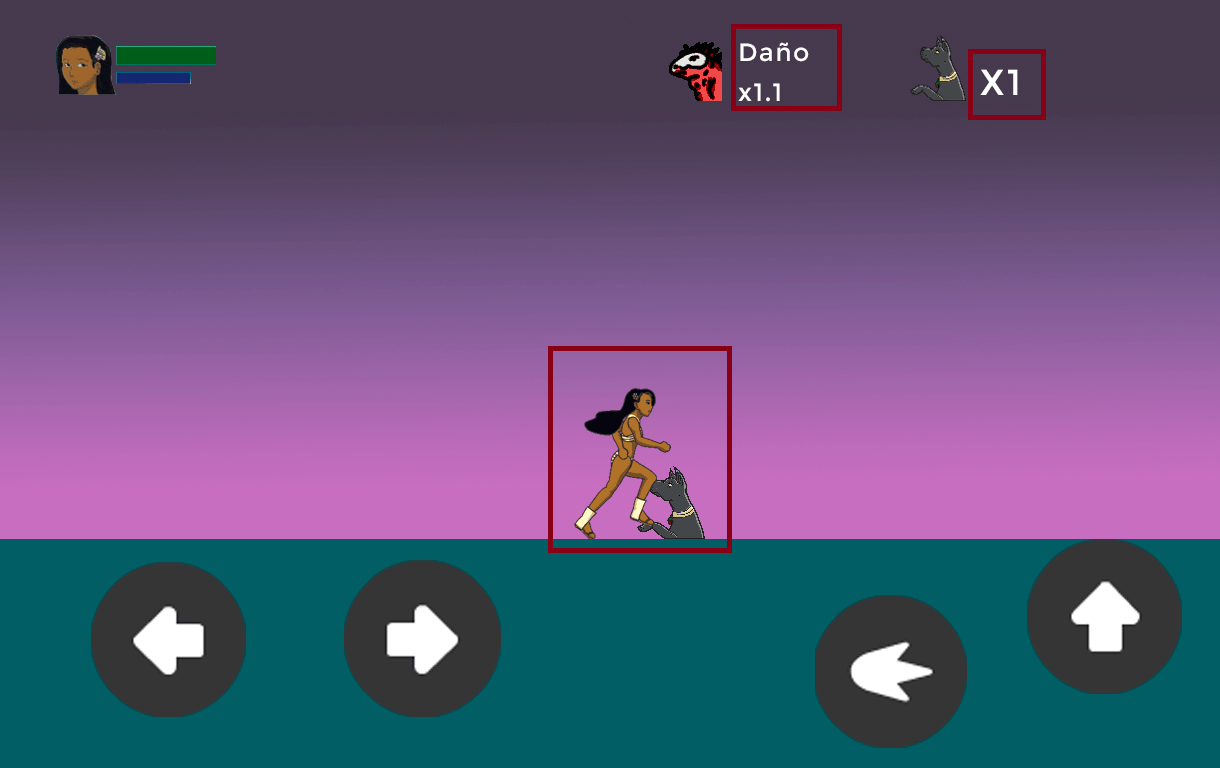
\includegraphics[width=0.4 \textwidth]{Imagenes/nivel02_xoloContacto}
  \caption{Cuando el jugador hace contacto con un Xoloitzcuintle los indicadores se modifican.}
  \label{fig:InterNivel2}
\end{figure} 

\begin{figure}
  \centering
   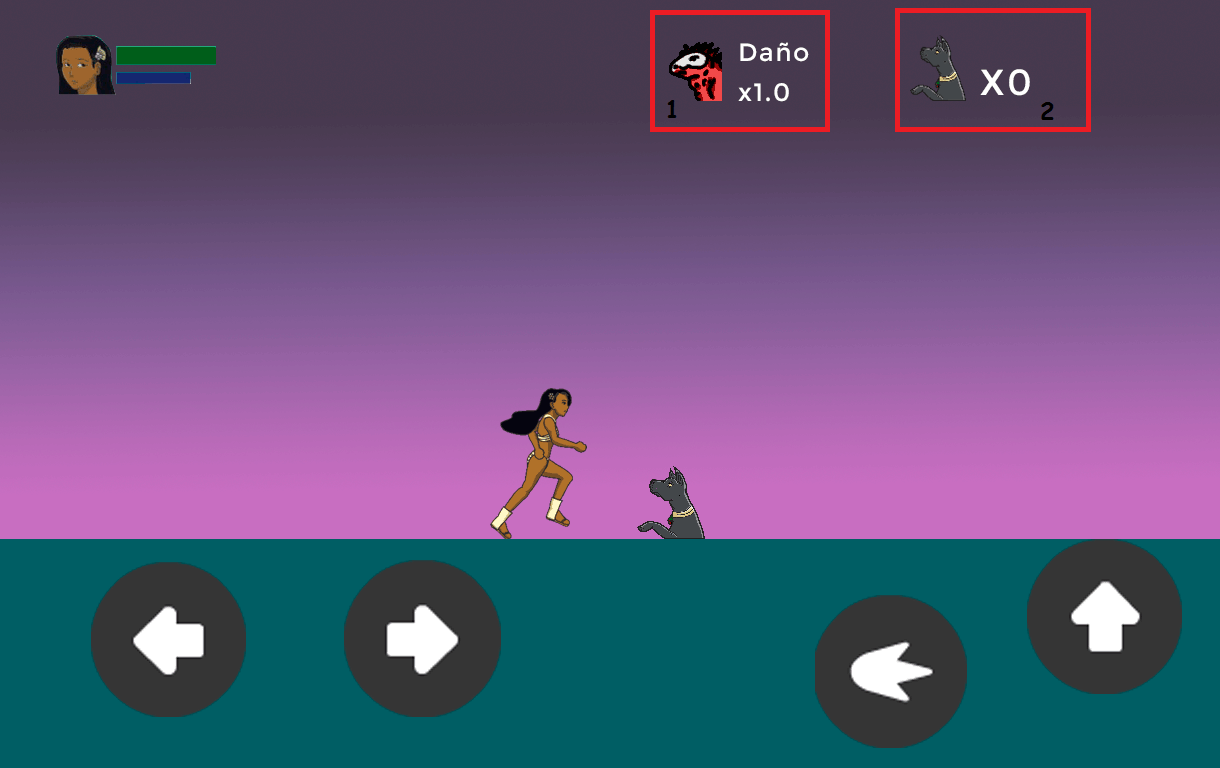
\includegraphics[width=0.4 \textwidth]{Imagenes/nivel02_xolo}
  \caption{1. Indicador de la cantidad de daño que puede efectuar Xochitonal. 2. Indicador de la cantidad de Xoloitzcuintles tocados.}
  \label{fig:GUICtrlNivel2}
\end{figure} 



	\subsection{Progreso}
Al final del nivel el jugador:
\begin{itemize}
	\item Obtendrá una mejora en la cantidad de vida de Malinalli.
	\item El jugador podrá ver las siguientes cinemáticas(Para mayor información sobre cada una, ver el guion literario del juego)
		\begin{itemize}
			\item Cinemática 6 (ver apartado \ref{Cin:Cinematica06}).
			\item Cinemática 7 (ver apartado \ref{Cin:Cinematica07}).
			\item Cinemática 8 (ver apartado \ref{Cin:Cinematica08}).
			\item Cinemática 9 (ver apartado \ref{Cin:Cinematica09}).
			\item Cinemática 10 (ver apartado \ref{Cin:Cinematica10}).
		\end{itemize}
	\item Tendrá disponible el tercer nivel del juego \ref{Nivel:Niv03} en el menú de selección de nivel (ver apartado \ref{inter:interfaz03}). 
\end{itemize}
	\subsection{Enemigos}
	\begin{itemize}
		\item Fantasma rojo (ver apartado \ref{per:fantasmaR}).
			
		\item Fantasma morado (ver apartado \ref{per:fantasmaM}).
			
		\item Piedras filosas (ver apartado \ref{obs:piedrasF}).
		\item Xochitonal (ver apartado \ref{per:xochitonal}).
			
	\end{itemize}
	\subsection{Items}
	\begin{itemize}
		\item Xoloitzcuintles (ver apartado\ref{item:Xolo}).
		\item Grano de cacao.
		\item Flor de vainilla.
	\end{itemize}
	\subsection{Personajes}
	\begin{itemize}
		\item Malinalli (ver apartado \ref{per:malinalli}).
		\item Xolotl (ver apartado \ref{per:xolotl}).
			
		\item Xochitonal (ver apartado \ref{per.xochitonal}).
	\end{itemize}
	
\subsection{Escenario}
\begin{itemize} 
	\item Fondo:
Montañas en el plano más alejado, y a sus pies una pequeña linea que muestre la orilla del río. El cielo es de color verde en degradado con negro.
	\item Suelo:
		\begin{itemize}
			\item Agua: Será utilizada durante la zona de plataformas y durante la batalla contra el jefe del nivel.
			\item Suelo con pasto: Será usado durante la cinemática 4 (ver apartado \ref{Cin:Cinematica04}) y la cinemática 8 (ver apartado \ref{Cin:Cinematica08}).
		\end{itemize}
	\item Obstáculos:
		\begin{itemize}
			\item Piedras filosas. Ver en \ref{obs.piedrasF}.				
		\end{itemize}
	\item Objetos de fondo: 
	\\
	\par	
	Sin objetos de fondo.
	
\end{itemize}	
	
	\subsection{Referencia a BGM y SFX}
\begin{itemize}
	\item BGM:
		\begin{itemize}
			\item Música plataforma segundo nivel (Ver apartado \ref{Musica:N02_ZN01})
			\item Música jefe segundo nivel (Ver apartado\ref{Musica:N02_ZN02}).
		\end{itemize}
	\item SFX:
		\begin{itemize}
			\item Explosión de agua (Ver apartado \ref{SFX:ExpAgua}).
			\item Salpicadura de agua (Ver apartado \ref{SFX:SalAgua}).
		\end{itemize}
\end{itemize}
	\subsection{Referencia a FX}
\begin{itemize}
	\item Oleaje (Ver apartado \ref{FX:Oleaje}).
	\item Salpucadura de agua (Ver apartado \ref{FX:SalAgua}).
	\item Explosión de burbuja (Ver apartado \ref{FX:ExpAgua}).
	\item Explosión de energía tonalli rojo (Ver apartado \ref{FX:ExpTonR}).
		 
\end{itemize}

		\section{Nivel 3}\label{Nivel:Niv03}
	\subsection{Título del nivel}
	La guarida del jaguar.	
	\subsection{Encuentro}
Este nivel estará disponible después de vencer al jefe del segundo nivel (ver apartado \ref{Nivel:Niv02}).
	\subsection{Descripción}
	Tras haber superado el primer nivel del Mictlán, Xólotl y Malinalli han llegado al Monamicyan, nivel gobernado por Tepeyóllotl. En este nivel Malinalli debera superar diferentes plataformas para llegar a la guarida de Tepeyóllotl y así obtener el poder del segundo guardián del infreamundo.
	\subsection{Objetivos}
	El jugador deberá:
\begin{itemize}
	\item Superar diferentes plataformas. En este nivel la exploración se hará de manera vertical, por lo que el espacio horizontal del nivel se vera reducido. A lo largo del nivel el jugador deberá coordinar los saltos de Malinalli para superar los obstáculos del nivel.
	\item Derrotar enemigos que protegen diferentes zonas del mapa, sin morir; cada enemigo infringirá una cantidad diferente de daño.
	\item Derrotar al jefe del nivel: Tepeyóllotl. Tepeyóllotl se encontrará protegido por su armadura de piedra por lo que sus ataques serán lentos, pero infringirán gran daño.
\end{itemize}
	\subsection{Progreso}
Al final del nivel el jugador:
\begin{itemize}
	\item Mejorará la cantidad de tonalli de Malinalli lo que permitirá usar más ataques con la caracola.
	\item Podrá ver las siguienteDesbloqueara una cinemática sobre el pasado de Malinallis cinemáticas: 
		\begin{itemize}
			\item Cinemática 12 (ver apartado \ref{Cin:Cinematica12}).
			\item Cinemática 13 (ver apartado \ref{Cin:Cinematica13}).
			\item Cinemática 14 (ver apartado \ref{Cin:Cinematica14}).
		\end{itemize}
	\item Desbloqueara el nivel cuatro (ver apartado \ref{Nivel:Niv04}) en el menú de selección de nivel (ver apartado \ref{inter:interfaz03}).
\end{itemize} 
	\subsection{Enemigos}
\begin{itemize}
	\item 	Fantasma rojo (ver apartado \ref{per:fantasmaR}).
		\begin{itemize}
				\item Animación fuego.
				\item Animación disparo.
			\end{itemize}
	\item Armadillo (ver apartado \ref{per:armadillo}).
		\begin{itemize}
			\item Animación de sacar picos.
			\item Animación rodar. 
		\end{itemize}
	\item Roca (ver apartado \ref{obs.rocas}).
		\begin{itemize}
			\item Animación romperse.
			\item Animación rodar.
		\end{itemize}
	\item Tepeyóllotl (ver apartado \ref{per:tepeyollotl}). 

\end{itemize}
	\subsection{Items}
\begin{itemize}
	\item 	Cacao.
	\item	Flor de vainilla.
\end{itemize}
	\subsection{Personajes}
\begin{itemize}
	\item Malinalli (ver apartado \ref{per:malinalli}).
		\begin{itemize}
			\item Animación correr.
			\item Animación saltar.
			\item Animación correr con caracola.
			\item Animación saltar con caracola.
			\item Animación normal.
			\item Animación recibir daño.
			\item Animación morir.
		\end{itemize}
	\item Xolotl (ver apartado \ref{per:xolotl}).
		\begin{itemize}
				\item Animación salto.
				\item Animación normal/nado.
		\end{itemize}
	\item Tepeyóllotl (ver apartado\ref{per:tepeyollotl}).
		\begin{itemize}
			\item Animación correr.
			\item Animación saltar.
			\item Animación rugir.
			\item Animación recibir daño.
			\item Animación morir.
		\end{itemize}
\end{itemize}
\subsection{Escenario}
\begin{itemize} 
	\item Fondo:
\begin{itemize}
	\item Bosque frondoso desde una perspectiva de tres puntos de fuga visto desde arriba. Tendrá un cielo azul despejado. A lo lejos se verá una montaña muy alta, con un templo en la cima.
\end{itemize}
	\item Suelo:
		\begin{itemize}
			\item Suelo con pasto.
		\end{itemize}
	\item Obstáculos:
		\begin{itemize}
			\item Plataforma móvil (ver apartado \ref{obs.plataformaM}).
			\item Plataforma que cae (ver apartado \ref{obs.plataformaD}).
		\end{itemize}
	\item Objetos de fondo:
		\begin{itemize}
			\item Arbusto.
			\item Árbol frágil.
		\end{itemize}
\end{itemize}	
	\subsection{Referencia a BGM y SFX}
\begin{itemize}
	\item BGM:
		\begin{itemize}
			\item Música plataforma tercer nivel (ver apartado\ref{Musica:N03_ZN01}).
			\item Nombre: Música jefe tercer nivel (ver apartado \ref{Musica:N03_ZN02}).
		\end{itemize}
	\item SFX:
		\begin{itemize}
			\item Viento (ver apartado \ref{SFX:Viento}).
			\item Rugido (ver apartado \ref{SFX:Rugido}).
			\item Roca estrellándose (ver apartado\ref{SFX:RocaEs}).
			\item Pasos (ver apartado \ref{SFX:Pasos})
		\end{itemize}
\end{itemize} 
	\subsection{Referencia FX}
\begin{itemize}
	\item Explosión de energía tonalli rojo (Ver apartado \ref{FX:ExpTonR}).
	\item Explosión de energía tonalli verde (Ver apartado \ref{FX:ExpTonV}).
\end{itemize}
		\section{Nivel 4} \label{Nivel:Niv04}
        \subsection{Título del nivel}
        Alas de obsidiana.
        \subsection{Encuentro}
Tercer nivel del inframundo, se desbloquea derrotando a Tepeyollótl en el tercer nivel (ver apartado \ref{Nivel:Niv03}).
        \subsection{Descripción}
        Luego de la huida de Tepeyollótl, Malinalli y Xólotl iniciarán una carrera contra el tiempo para poder llegar a su segunda guarida y evitar que contacte a Tezcatlipoca pero primero deberán superar el Itztépetl, hogar de Itzpapálotl. Así deberán adentrarse en las profundidades de una cueva para encontrar templo subterráneo donde se esconde Itzpapálotl. 
        \subsection{Objetivos}
En este nivel el jugador deberá:        
\begin{itemize}
        \item Descubrir el camino correcto hacia el templo de Itzpapálotl, el jugador podrá explorar de manera horizontal y vertical el nivel. A manera de ayudarle al jugador a encontrar el camino, habrá pequeñas mariposas azules en las zonas del mapa que correspondan al camino hacia la guarida de Itzpapálotl. 
        \item Encontrar tres llaves que permiten abrir la entrada a la guarida de Itzpapálotl. Cada llave estará oculta en una zona del mapa custodiada por un enemigo. El jugador deberá de derrotar al enemigo que protege la llave, una vez derrotado el enemigo, éste explotará dejando caer la llave en la posición en la que se encontraba al momento de ser derrotado. Una vez que el jugador derrote al enemigo, deberá de colisionar con la llave para obtenerla. Cuando el jugador colisione con la llave el contador que lleva el control de cuantas llaves ha recogido el jugador se actualizara en uno. El contador de las llaves se ubicará en la parte superior derecha de la pantalla precedido por el icono de la llave. 
        \item Superar las diferentes plataformas y obstáculos que hay en el laberinto. 
        \item Derrotar a los enemigos que hay en el laberinto.
        \item Derrotar a Itzpapálotl.
\end{itemize}
        \subsection{Progreso}
Al final del nivel el jugador:
\begin{itemize}
        \item Aumentará la cantidad de vida de Malinalli.
        \item Desbloquear las siguientes cinemáticas:
		\begin{itemize}
			\item Cinemática 16 (ver apartado \ref{Cin:Cinematica16}).
			\item Cinemática 17 (ver apartado \ref{Cin:Cinematica17}).
			\item Cinemática 18 (ver apartado \ref{Cin:Cinematica18}).
			\item Cinemática 19 (ver apartado \ref{Cin:Cinematica19}).
			\item Cinemática 20 (ver apartado \ref{Cin:Cinematica20}).
			\item Cinemática 21 (ver apartado \ref{Cin:Cinematica21}).
			\item Cinemática 22 (ver apartado \ref{Cin:Cinematica22}).
		\end{itemize}
        \item Desbloquear El nivel 5 (ver apartado \ref{Nivel:Niv05}) del juego en el menú seleccionable (ver apartado \ref{inter:interfaz03}).
\end{itemize}        
        \subsection{Enemigos}
                \begin{itemize}
                    \item Fantasma rojo. Ver en \ref{per:fantasmaR}. 
            
					\item Fantasma morado (ver apartado \ref{per:fantasmaM}).
			\begin{itemize}
				\item Animación fuego.
			\end{itemize}
            \item Picos de obsidiana (ver apartado \ref{obs:piedrasF}).
             \item Itzpapalotl (ver apartado \ref{per:itzpapalotl}).
                \end{itemize}
        \subsection{Items}
                \begin{itemize}
                        \item   Cacao (ver apartado \ref{item:cacao}).
                        \item Flor de Vainilla (ver apartado \ref{item:vainilla}).
                        \item Llave a la guarida de Itzpapálotl.
                        \item Mariposa azul (ver apartado \ref{item:Mariposa})
                \end{itemize}
        \subsection{Personajes}
        \begin{itemize}
                \item Malinalli (ver apartado \ref{per:malinalli}).
            
                \item Xolotl (ver apartado \ref{per:xolotl}).
                
                \item Itzpapalotl (ver apartado \ref{per:itzpapalotl}).
               
        \end{itemize}
\subsection{Escenario}
\begin{itemize} 
        \item Fondo:
                \begin{itemize}
                        \item Zona de plataformas:
\\
\par
El nivel esta ubicado en el subterráneo, el fondo deberá parecer a una mina con cristales de luz verde que salen del suelo y de la pared.
                        \item Zona del jefe:
Es el interior del templo,el templos solo es iluminado por los cristales verdes. La batalla se desarrollara en un cuarto de entrenamiento por lo que habrán diferentes armas en las paredes.
                \end{itemize}
        \item Suelo:
                \begin{itemize}
                        \item Suelo rocoso: Para la zona de las plataformas.
                        \item Suelo pavimentado: Zona jefe.
                \end{itemize}
	  \item Obstáculos:
                \begin{itemize}
                        \item Viento (ver apartado \ref{obs.vientoT}).
                \end{itemize}
        \item Objetos de fondo:
                \begin{itemize}
                        \item Cristal verde: Cristal de luz verde que ilumina algunas zonas de la cueva.
                \end{itemize}
\end{itemize}   

        \subsection{Referencia a BGM y SFX}
                \begin{itemize}
                        \item BGM.
                \begin{itemize}
                        \item Música plataforma cuarto nivel (ver apartado \ref{Musica:N04_ZN01}).
				\item Música jefe cuarto nivel (ver apartado \ref{Musica:N04_ZN02})
                \end{itemize}
				\item SFX.
                \begin{itemize}
                        \item Aleteo de alas (ver apartado \ref{SFX:Aleteo}).
                        \item Viento (ver apartado\ref{SFX:Viento}).
                        \item Sonido de fuego (ver apartado \ref{SFX:Fuego}).			
                \end{itemize}
                \end{itemize}

        \subsection{Referencia a FX}
\begin{itemize}    
	\item Explosión de energía tonalli rojo (Ver apartado \ref{FX:ExpTonR})
	\item Explosión de energía tonalli verde (Ver apartado \ref{FX:ExpTonV})
    \item Haz de luz \ref{FX:HazLuz}
    
\end{itemize}
		\section{Nivel 5} \label{Nivel:Niv05}
        \subsection{Título del nivel}
        Cehuelóyan: Lugar donde hay mucha nieve
        \subsection{Encuentro}
        Este nivel se desbloqueara después de haber terminado el Nivel 4.
        \subsection{Descripción}
Malinalli y Xólotl han llegado al Cehuelóyan, nivel del Mictlán custodiad por Mictlecayotl. Lo primero en recibirlos es el gélido viento de la zona pero no hay tiempo para lamentar el clima. Malinalli deberá mantener ambos ojos bien abiertos y coordinar cada movimiento ya que cada centímetro de nieve puede ser un lugar seguro o sitio frágil que caerá al vació.      
        \subsection{Objetivos}
En este nivel el jugador deberá:
\begin{itemize}
        \item Superar las diferentes plataformas. El nivel estará más centrado en las plataformas que en derrotar enemigos. Nuevamente el juego vuelve a implementar una progresión horizontal para la exploración. 
        \item  Derrotar a Mictlecayotl. La batalla contra el jefe de zona se desarrollará en una serie de plataformas que modificaran su posición cada determinado tiempo o desaparecerán. El jugador deberá saltar constantemente para no caer de la plataformas mientras ataca a Mictlecayotl y a su vez deberá evitar los ataques de la diosa.
\end{itemize}


        \subsection{Progreso}
        Al terminar el nivel el jugador:
\begin{itemize}
        \item Habrá incrementado la energía espiritual de Malinalli. 
        \item Desbloqueara las siguientes cinemáticas:
\begin{itemize}
        \item Cinemática 24 (ver apartado \ref{Cin:Cinematica24}). 
        \item Cinemática 25 (ver apartado \ref{Cin:Cinematica25}).
        \item Cinemática 26 (ver apartado \ref{Cin:Cinematica26}).
        \item Cinemática 27 (ver apartado \ref{Cin:Cinematica27}).
\end{itemize}
        \item Desbloqueará El nivel 6 (ver apartado  \ref{Nivel:Niv06}) del juego en el menú seleccionable (ver apartado \ref{inter:interfaz03}).
\end{itemize}

        \subsection{Enemigos}
\begin{itemize}
        \item Fantasma morado (ver apartado \ref{per:fantasmaM}).
        \begin{itemize}
				\item Animación fuego.
		\end{itemize}
        \item Chara enana  (ver apartado \ref{per:chara}).
        \begin{itemize}
				\item Animación vuelo.
				\item Animación caída en picada.
		\end{itemize}
		\item Mictlecayotl (ver apartado \ref{per:mictlecayotl}).
\begin{itemize}
        \item Animación volar.
        \item Animación disparar viento.
        \item Animación invocar tornado.
        \item Animación volar.
        \item Animación recibir daño.
		\item Animación morir.
\end{itemize}			
\end{itemize}
        \subsection{Items}
\begin{itemize}
        \item   Cacao (ver apartado \ref{item:cacao}).
        \item Flor de Vainilla (ver apartado \ref{item:vainilla}).
\end{itemize}
        \subsection{Personajes}
        \begin{itemize}
                \item Malinalli. Ver en \ref{per:malinalli}.
                \begin{itemize}
                        \item Animación correr.
                        \item Animación saltar.
                        \item Animación correr caracola.
                        \item Animación saltar caracola.
                        \item Animación normal.
                        \item Animación recibir daño.
						\item Animación morir.
                \end{itemize} 
                \item Xolotl. Ver en \ref{per:xolotl}.
                \begin{itemize}
					\item Animación salto.
					\item Animación normal.
				\end{itemize}
                \item Mictlecayotl. Ver en \ref{per:mictlecayotl}.
                \begin{itemize}
                        \item Animación disparar viento.
                        \item Animación invocar tornado.
                        \item Animación volar.
                        \item Animación recibir daño.
						\item Animación morir.
                \end{itemize} 
        \end{itemize}
        \subsection{Escenario}
\begin{itemize} 
        \item Fondo:
\begin{itemize} 
        \item El fondo son montañas cubiertas de nieve. El cielo es nublado sin la posibilidad de estar seguro en que momento del día es, las nubes de este nivel son de color azul claro, como la nieve.
\end{itemize} 
        \item Suelo:
\begin{itemize} 
        \item Suelo cubierto de nieve.
\end{itemize} 
        \item Obstáculos:
			\item Plataforma móvil (ver apartado \ref{obs.plataformaM}).
			\item Plataforma que cae (ver apartado \ref{obs.plataformaD}).
			\item Piso resbaladizo. (ver apartado \ref{obs.pisoC}).
			\item Plataforma que desaparece (ver apartado \ref{obs.PlatDes}).
			\item Bola de nieve (ver apartado \ref{obs.bolasN}).
		\end{itemize}
        \item Objetos de fondo: Sin objetos de fondo.
\end{itemize}   
        \subsection{Referencia a BGM y SFX}
\begin{itemize} 
        \item BGM:
\begin{itemize} 
        \item Música plataforma quinto nivel (ver apartado \ref{Musica:N05_ZN01}).
        \item Música jefe quinto nivel (ver apartado \ref{Musica:N05_ZN02}).
\end{itemize}
        \item SFX:
\begin{itemize} 
        \item Viento (ver apartado \ref{SFX:Viento}).
        \item Hielo resquebrajándose (ver apartado \ref{SFX:HieloRes}).
        \item Pasos sobre el hielo o la nieve(ver apartado \ref{SFX:PasHiel}).	
\end{itemize}
\end{itemize}

        \subsection{Referencia a FX}
\begin{itemize} 
        \item Ventisca de nieve: (ver apartado \ref{FX:VenNieve}).
        \item Explosión de energía tonalli rojo (Ver apartado \ref{FX:ExpTonR})
	\item Explosión de energía tonalli verde (Ver apartado \ref{FX:ExpTonV})
	\item Respiración (\ref{Ver apartado SFX:Respiracion}) 
\end{itemize} 
			\section{Nivel 6} \label{Nivel:Niv06}
	\subsection{Título del nivel}
	Sin gravedad.
	\subsection{Encuentro}
	Este nivel estará disponible después de vencer al jefe del quinto nivel (ver apartado \ref{Nivel:Niv05}).
	\subsection{Descripción}
	A la entrada del Pancuetlacalóyan, Xólotl le advierte a Malinalli sobre los peligros que los esperan en los dominios de Tlazoltéotl. Para ayudar a Malinalli, Xólotl adopta la forma de un ave. Juntos surcaran los cielos del Pancuetlacalóyan con el objetivo de reclamar el poder de Tlazoltéotl.
	\subsection{Objetivos}
	En este nivel el jugador:
	\begin{itemize}
		\item Atravesar la zona de plataformas del nivel. En este nivel Xólotl (ver aparatado \ref{per:xolotl}) se transformara en un ave y surcara el nivel volando por lo que el jugador deberá de mantenerse sobre él para poder avanzar. Xólotl contara con una velocidad predefinida y el jugador no la podrá modificar, Xólotl sólo disminuirá su velocidad en las zonas con enemigos para darle tiempo al jugador de poder centrarse en la batalla o en las zonas de plataformas para que el jugador pueda obtener ítems. Xólotl contará con una barra de vida parecida a la de Malinalli, esta barra estará ubicada en la parte superior derecha de la pantalla y estará precedida por la imagen de Xólotl. La cantidad de vida de Xólotl disminuirá si colisiona con  los enemigos o con sus ataques; si la barra de vida de Xólotl llega cero, éste desaparecerá y el jugador perderá la partida. Al igual que Malinalli, Xólotl podrá recuperar vida con el ítem grano de cacao (ver apartado \ref{item:cacao}).
		\item Derrotar a Tlazoltéotl. Tlazoltéotl aparecerá volando y Xólotl la seguirá. El jugador deberá evitar los ataques de la diosa sin caerse de Xólotl. Tlazoltéotl estará rodeada de un circulo de tonalli corrupto, por lo que el jugador deberá disparar tonalli para destruir el circulo que protege a Tlazoltéotl. Tlazoltéotl será inmune a cualquier ataque mientras se encuentre activo el circulo de tonalli corrupto; una vez destruido el circulo de tonalli corrupto, los ataques del jugador podrán herir a Tlazoltéotl. Tlazoltéotl estará sin el circulo de tonalli corrupto por un tiempo y después lo volverá a invocar. 
	\end{itemize}	 
	\subsection{Progreso}
	 Al terminar el nivel el jugador:
\begin{itemize}
        \item Habrá incrementado la cantidad de vida de Malinalli. 
        \item Desbloqueara las siguientes cinemáticas:
\begin{itemize}
        \item Cinemática 29 (ver apartado \ref{Cin:Cinematica29}). 
        \item Cinemática 30 (ver apartado \ref{Cin:Cinematica30}).
        \item Cinemática 31 (ver apartado \ref{Cin:Cinematica31}).
\end{itemize}
        \item Desbloqueará El nivel 7 (ver apartado  \ref{Nivel:Niv07}) del juego en el menú seleccionable (ver apartado \ref{inter:interfaz03}).
\end{itemize}
	\subsection{Enemigos}
	\begin{itemize}
		\item Fantasmas rojos. Ver en \ref{per:fantasmaR}.
			\begin{itemize}
				\item Animación fuego.
				\item Animación disparo.
			\end{itemize}
		\item Tlazoltéotl. Ver en \ref{per:tlazolteotl}.
	\end{itemize}
	\subsection{Items}
\begin{itemize}
        \item   Cacao (ver apartado \ref{item:cacao}).
        \item Flor de Vainilla (ver apartado \ref{item:vainilla}).
\end{itemize}
	\subsection{Personajes}
	\begin{itemize}
		\item Malinalli. Ver en \ref{per:malinalli}.
			\begin{itemize}
			\item Animación correr.
			\item Animación saltar.
			\item Animación correr con caracola.
			\item Animación saltar con caracola.
			\item Animación normal.
			\item Animación recibir daño.
			\item Animación morir.
		\end{itemize}
		\item Xolotl. Ver en \ref{per:xolotl}.
		\begin{itemize}
				\item Animación salto.
				\item Animación normal.
		\end{itemize}
		\item Tlazoltéotl. Ver en \ref{per:tlazolteotl}.
			\begin{itemize}
				\item Animación vuelo.
				\item Animación disparar energía corrupta.
				\item Animación invocar círculo protector.
				\item Animación disparar raíz diablo.
				\item Animación recibir daño.
				\item Animación morir.
			\end{itemize}
	\end{itemize}
\subsection{Escenario}
\begin{itemize} 
	\item Fondo: El cielo de este nivel es de color rojo. Las nubes se observan a la lejanía formando un espiral y bajo ellas se pueden observar varios truenos que caen sobre montañas.
	\item Suelo: Rocoso obscuro.
	\item Obstáculos: Caer al vacío.
	\item Viento en contra. Ver en \ref{obs.vientoM}.
	\item Objetos de fondo: Sin objetos de fondo
\end{itemize}	
	\subsection{Referencia a BGM y SFX}
	\begin{itemize}
		\item BGM
			\begin{itemize}
				\item Música plataforma sexto nivel (ver apartado \ref{Musica:N06_ZN01}).
				\item Música jefe sexto nivel (ver apartado \ref{Musica:N06_ZN02}).
			\end{itemize}
		\item SFX
		\begin{itemize}
			\item Risa de mujer (ver apartado \ref{SFX:risaM}).
			\item Viento (ver apartado \ref{SFX:Viento}).
			\item Liquido viscoso (ver apartado \ref{SFX:ligVisc}).
		\end{itemize}
	\end{itemize}
	\subsection{Referencia a FX}
	\begin{itemize}
		\item Explosión de Tonalli corrupto (ver apartado \ref{FX:ExTonCor}).
		\item Explosión de energía tonalli rojo (ver apartado \ref{FX:ExpTonR})
	\item Explosión de energía tonalli verde (ver apartado \ref{FX:ExpTonV})
	\item Relámpagos (ver apartado \ref{FX:Relam}).
	\end{itemize}
	
		\section{Nivel 7}  \label{Nivel:Niv07}
	\subsection{Título del nivel}
	Castigo.
	\subsection{Encuentro}
	Este nivel estará disponible después de vencer al jefe del noveno sexto (ver apartado \ref{Nivel:Niv06}).
	\subsection{Descripción}
	Malinalli y Xólotl se adentran en los dominios de Itztlacoliuhqui. Xolotl sabe que deben de avanzar con cautela pues Itztlacoliuhqui los espera con deseos de vengar la muerte de Itzpápalotl. Malinalli y Xolotl deberán cruzar Temiminalóyan y los peligros que trae consigo.
	\subsection{Objetivos}
	\begin{itemize}
		\item Atravesar la zona de plataformas. En este nivel lloverán flechas de manera periódica, por lo que el jugador deberá de avanzar de forma cautelosa y refugiarse en las zonas seguras durante la lluvia de flechas. En la parte superior derecha de la pantalla habrá una barra que se ira llenando, cuando la barra este llena iniciara la lluvia de flechas, el jugador podrá atrasar el llenado de la barra destruyendo las estatuas del sol que están distribuidas por el nivel.  
		\item Derrotar a Itztlacoliuhqui. En la batalla contra Itztlacoliuhqui, éste incrementara su tamaño transformándose en una versión gigantesca de sí mismo.  Por lo que el jugador deberá de subir una serie de plataformas para atacar la cabeza de Itztlacoliuhqui, siendo este punto el único en donde Itztlacoliuhqui disminuirá su barra de vida. Las plataformas que hay en esta batalla serán del tipo de las que aparecen y desaparecen con el tiempo. La barra que indica cuando llueven flechas se mantendrá, pero se llenará más rápido que en la zona de plataformas.
	\end{itemize}
	\subsection{Progreso}
	Al terminar el nivel el jugador:
\begin{itemize}
        \item Habrá incrementado la cantidad de tonalli de Malinalli. 
        \item Desbloqueara las siguientes cinemáticas:
\begin{itemize}
        \item Cinemática 33 (ver apartado \ref{Cin:Cinematica33}). 
        \item Cinemática 34 (ver apartado \ref{Cin:Cinematica34}).
        \item Cinemática 35 (ver apartado \ref{Cin:Cinematica35}).
\end{itemize}
        \item Desbloqueará El nivel 8 (ver apartado  \ref{Nivel:Niv08}) del juego en el menú seleccionable (ver apartado \ref{inter:interfaz03}).
\end{itemize} 
	\subsection{Enemigos}
	\begin{itemize}
		\item Fantasmas morados. Ver en \ref{per:fantasmaM}.
			\begin{itemize}
				\item Animación fuego.
			\end{itemize}
		\item Fantasmas rojos. Ver en \ref{per:fantasmaR}.
		\begin{itemize}
				\item Animación fuego.
				\item Animación disparo.
			\end{itemize}
		\item Itztlacoliuhqui. Ver en \ref{per:itztlacoliuhqui}.
	\end{itemize}
	\subsection{Items}
\begin{itemize}
        \item   Cacao (ver apartado \ref{item:cacao}).
        \item Flor de Vainilla (ver apartado \ref{item:vainilla}).
\end{itemize}
	\subsection{Personajes}
	\begin{itemize}
		\item Malinalli. Ver en \ref{per:malinalli}.
		\begin{itemize}
			\item Animación correr.
			\item Animación saltar.
			\item Animación correr con caracola.
			\item Animación saltar con caracola.
			\item Animación normal.
			\item Animación recibir daño.
			\item Animación morir.
		\end{itemize}
		\item Xolotl. Ver en \ref{per:xolotl}.
		\begin{itemize}
				\item Animación salto.
				\item Animación normal.
		\end{itemize}
		\item Itztlacoliuhqui. Ver en \ref{per:itztlacoliuhqui}.
		\begin{itemize}
			\item Animación manotazo.
			\item Animación lanzar lava.
			\item Animación invocar flechas.
		\end{itemize}
	\end{itemize}
	\subsection{Escenario}
\begin{itemize} 
	\item Fondo: A lo lejos se verá un volcán en erupción. El cielo es un perpetuo atardecer. Se observan montañas sin vegetación y una amplia meseta seca, cuyo suelo se muestra cuarteado denotando que la zona está pasando por un periodo de sequía. 
	\item Suelo: Piso rocoso y rocoso agrietado.
	\item Obstáculos:
	\begin{itemize}
	\item Plataforma móvil (ver apartado \ref{obs.plataformaM}).
			\item Plataforma que cae (ver apartado \ref{obs.plataformaD}).
			\item Lluvia de flechas (ver apartado \ref{obs.lluviaF}).
\end{itemize}	 
	
	\item Objetos de fondo: Sin objetos de fondo.
\end{itemize}	
	\subsection{Referencia a BGM y SFX}
	\begin{itemize}
		\item BGM
			\begin{itemize}
				\item Música plataforma séptimo nivel (ver apartado \ref{Musica:N07_ZN01}).
				\item Música jefe séptimo nivel (ver apartado \ref{Musica:N07_ZN02}).
			\end{itemize}
		\item SFX
			\begin{itemize}
				\item Pasos (ver aparatado \ref{SFX:Pasos})
				\item Viento (ver apartado \ref{SFX:Viento}).
				\item Golpe (ver apartado \ref{SFX:golpe}).
			\end{itemize}
			\item Silbido (ver apartado \ref{SFX:silbido}).
	\end{itemize}
	\subsection{Referencia a FX}
	\begin{itemize}
		\item Explosión de energía tonalli rojo (ver apartado \ref{FX:ExpTonR})
	\item Explosión de energía tonalli verde (ver apartado \ref{FX:ExpTonV})
	\item Temblor (ver apartado \ref{FX:temblor}).
	\item Cámara obscura (ver apartado \ref{FX:CamObs}).
	\end{itemize}
	
			\section{Nivel 8} \label{Nivel:Niv08}
	\subsection{Título del nivel}
	La última batalla del jaguar.
	\subsection{Encuentro}
	Este nivel estará disponible después de vencer al jefe del séptimo nivel (ver apartado \ref{Nivel:Niv08}).
	\subsection{Descripción}
	Malinalli irá por un camino selvático que deberá atravesar. Se enfrentará de nuevo con Tepeyollotl ahora sin armadura de piedra.
	\subsection{Objetivos}
	El jugador deberá:
	\begin{itemize}
		\item Superar la zona de plataformas. El suelo del nivel tendrá dos tipos de sprites para el suelo, uno pavimentado y otro con pasto. Los enemigos que se encuentren en la zona con pasto serán más fuertes que los enemigos que se encuentren en la zona pavimentada. 
		\item Derrotar a Tepeyóllotl. En esta batalla contra jefe, Tepeyóllotl no tendrá su coraza por lo que sus ataque serán más rápidos que los del segundo nivel (ver apartado \ref{Nivel:Niv02}).
	\end{itemize}
	\subsection{Progreso}
	Al terminar el nivel el jugador:
\begin{itemize}
        \item Habrá incrementado la cantidad de vida de Malinalli. 
        \item Desbloqueara las siguientes cinemáticas:
\begin{itemize}
        \item Cinemática 37 (ver apartado \ref{Cin:Cinematica37}). 
        \item Cinemática 38 (ver apartado \ref{Cin:Cinematica38}).
        \item Cinemática 39 (ver apartado \ref{Cin:Cinematica39}).
        \item Cinemática 40 (ver apartado \ref{Cin:Cinematica40}).
\end{itemize}
        \item Desbloqueará El nivel 9 (ver apartado  \ref{Nivel:Niv09}) del juego en el menú seleccionable (ver apartado \ref{inter:interfaz03}).
\end{itemize}
	\subsection{Enemigos}
	\begin{itemize}
		\item Jaguar. Ver en \ref{per:jaguar}.
			\begin{itemize}
				\item Animación atacar.
				\item Animación caminar.
			\end{itemize}
		\item Fantasmas morados. Ver en \ref{per:fantasmaM}.
			\begin{itemize}
				\item Animación fuego.
			\end{itemize}
		\item Fantasmas rojos. Ver en \ref{per:fantasmaR}.
			\begin{itemize}
				\item Animación fuego.
			\end{itemize}
		\item Tepeyóllotl. Ver en \ref{per:tepeyollotl}.
	\end{itemize}
	\subsection{Items}
	\begin{itemize}
        \item   Cacao (ver apartado \ref{item:cacao}).
        \item Flor de Vainilla (ver apartado \ref{item:vainilla}).
\end{itemize}
	\subsection{Personajes}
	\begin{itemize}
		\item Malinalli. Ver en \ref{per:malinalli}.
		\begin{itemize}
			\item Animación correr.
			\item Animación saltar.
			\item Animación correr con caracola.
			\item Animación saltar con caracola.
			\item Animación normal.
			\item Animación recibir daño.
			\item Animación morir.
		\end{itemize} 
		\item Xolotl. Ver en \ref{per:xolotl}.
		\begin{itemize}
				\item Animación salto.
				\item Animación normal.
		\end{itemize}
		\item Tepeyóllotl. Ver en \ref{per:tepeyollotl}.
		\begin{itemize}
			\item Animación correr (sin coraza).
			\item Animación saltar (sin coraza).
			\item Animación rugir (sin coraza).
			\item Animación recibir daño (sin coraza).
			\item Animación morir (sin coraza).
		\end{itemize}
	\end{itemize}
	\subsection{Escenario}
\begin{itemize} 
	\item Fondo: .
	\item Suelo: Piso selvático, de roca blanca y roca blanca agrietada.
	\item Obstáculos:
	\begin{itemize}
		item Plataforma móvil (ver apartado \ref{obs.plataformaM}).
			\item Plataforma que cae (ver apartado \ref{obs.plataformaD}).
	\end{itemize}
	\item Objetos de fondo: No hay
\end{itemize}		
	\subsection{Referencia a BGM y SFX}
	\begin{itemize}
	\item BGM
		\begin{itemize}
				\item Música plataforma octavo nivel (ver apartado \ref{Musica:N08_ZN01}).
				\item Música jefe octavo nivel (ver apartado \ref{Musica:N08_ZN02}).
			\end{itemize}
		\item SFX
		\begin{itemize}
			\item Viento (ver apartado \ref{SFX:Viento}).
			\item Rugido (ver apartado \ref{SFX:Rugido}).
			\item Roca estrellándose (ver apartado\ref{SFX:RocaEs}).
			\item Pasos (ver apartado \ref{SFX:Pasos})
		\end{itemize}
\end{itemize} 
	\end{itemize}
	\subsection{Referencia a FX}
\begin{itemize}
	\item Explosión de energía tonalli rojo (Ver apartado \ref{FX:ExpTonR}).
	\item Explosión de energía tonalli verde (Ver apartado \ref{FX:ExpTonV}).
\end{itemize}
	
			\section{Nivel 9} \label{Nivel:Niv09}
	\subsection{Título del nivel}
	El último caballero del rey.
	\subsection{Encuentro}
	Este nivel estará disponible después de vencer al jefe del octavo nivel (ver apartado \ref{Nivel:Niv08}).  
	\subsection{Descripción}
	Luego de derrotar a Tepeyóllotl, Malinalli y Xólotl se dirigen hacia el penúltimo nivel del Mictlán. Éste nivel promete ser el más difícil para ambos, pues esta vez el enemigo a vencer no serán seres mágicos sino sus propios miedos y demonios internos.
	\\
\par
Este es el único nivel que está dividido en tres etapas, dos de plataformas y una de batalla contra el jefe. Siendo también el único nivel en el que se tendrá dos personajes jugables: Xólotl para la primera etapa de plataformas y Malinalli para la segunda etapa de plataformas y la batalla contra el jefe.

	\subsection{Objetivos}
	El jugador deberá:	
	\begin{itemize}
		\item Superar la zona de Tula. Zona en la que el jugador deberá de controlar a Xólotl. El jugador explorará la ciudad de Tula, en donde deberá seguir a la figura de Quetzalcóatl por varias zonas de la ciudad. Durante la persecución de Quetzalcóatl le dirá mostrará diferentes diálogos en donde contará la relación que tenía con Xólotl.
		\item Superar la zona de Oluta. En esta zona el jugador controlara a Malinalli. El jugador explorará el palacio de Oluta, en donde seguirá a Malinalli versión niña. En esta zona el jugador tendrá que dialogar con algunos de los  habitantes del palacio para poder avanzar entre las habitaciones del palacio.
		\item Derrotar a Nexoxcho. Nexoxcho tomará la forma del padre de Malinalli para torturarla psicológicamente.  El jugador deberá de enfrentar a Nexoxcho, sin embargo, por el estado emocional de Malinalli, la velocidad a la que se mueve el jugador serán más lenta, la capacidad de salto se reducirá y el gasto de tonalli por disparo se infrementará.
	\end{itemize}
	\subsection{Progreso}
		Al terminar el nivel el jugador:
\begin{itemize}
        \item Habrá incrementado la cantidad de vida de Malinalli. 
        \item Desbloqueara las siguientes cinemáticas:
\begin{itemize}
        \item Cinemática 44 (ver apartado \ref{Cin:Cinematica44}). 
        \item Cinemática 45 (ver apartado \ref{Cin:Cinematica45}).
        \item Cinemática 46 (ver apartado \ref{Cin:Cinematica46}).
\end{itemize}
        \item Desbloqueará El nivel 10 (ver apartado  \ref{Nivel:Niv10}) del juego en el menú seleccionable (ver apartado \ref{inter:interfaz03}). 
 \end{itemize}
	\subsection{Enemigos}
	\begin{itemize}
		\item Fantasmas rojos (ver apartado \ref{per:fantasmaR}).
		\begin{itemize}
				\item Animación fuego.
				\item Animación disparo.
			\end{itemize}
		\item Fantasmas morados (ver apartado \ref{per:fantasmaM}).
		\begin{itemize}
				\item Animación fuego.
			\end{itemize}
		\item Deidades. Ver en ??.
		\item Nexchocho (ver apartado \ref{per:nexoxcho}).
	\end{itemize}
	\subsection{Items}
\begin{itemize}
        \item   Cacao (ver apartado \ref{item:cacao}).
        \item Flor de Vainilla (ver apartado \ref{item:vainilla}).
\end{itemize}
	\subsection{Personajes}
	\begin{itemize}
		\item Malinalli (ver apartado \ref{per:malinalli}).
		\begin{itemize}
			\item Animación correr.
			\item Animación saltar.
			\item Animación correr con caracola.
			\item Animación saltar con caracola.
			\item Animación normal.
			\item Animación recibir daño.
			\item Animación morir.
		\end{itemize}
		\item Xólotl (ver apartado \ref{per:xolotl}).
		\begin{itemize}
				\item Animación salto.
				\item Animación normal.
		\end{itemize}
		\item Nexchocho (ver apartado \ref{per:nexoxcho}).
		\begin{itemize}
			\item Animación apuñalar.
			\item Animación caminar.
			\item Animación recibir daño.
			\item Animación morir.
		\end{itemize}
	\end{itemize}
	\subsection{Escenario}
\begin{itemize} 
	\item Fondo: 
		\begin{itemize}
			\item Ciudad de Tula: Se mostraran casa, calles y personas de fondo en plano más cercano al jugador. A lo lejos se verán grandes templos y más edificaciones que muestren el esplendor de la ciudad. Se puede ver un cielo nocturno despejado.
			\item Ciudad de Tula destruida: Las edificaciones de la ciudad veían ahora están parcialmente destruidas o destruidas. Hay fuego y personas en el suelo o corriendo. Se puede ver un cielo nocturno apocado por el humo de la ciudad.
			\item Interior del palacio de Oluta: El cielo que se ve por las ventanas es nocturno. Hay antorchas iluminando el interior del palacio, de las paredes cuelgan finas telas de colores.
		\end{itemize}
	\item Suelo: Roca negra, agua negra.
	\item Obstáculos: Sin obstáculos.
	\item Objetos de fondo: Sin objetos.
\end{itemize}	
	\subsection{Referencia a BGM y SFX}
	\begin{itemize}
		\item BGM.
			\begin{itemize}
				\item Música plataforma noveno nivel, Tula (ver apartado \ref{Musica:N09_ZN01T}).
				\item Música plataforma noveno nivel, Oluta primera etapa (ver apartado \ref{Musica:N09_ZN01C}).
				\item Música plataforma noveno nivel, Oluta segunda etapa (ver apartado \ref{Musica:N09_ZN01C02}).
				\item Música jefe noveno nivel (ver apartado \ref{Musica:N09_ZN02}).
			\end{itemize}
		\item SFX.
			\begin{itemize}
				\item Pasos (ver apartado \ref{SFX:Pasos}).
				\item Viento (ver apartado \ref{SFX:Viento}).
				\item Sonido de fuego (ver apartado \ref{SFX:Fuego}).
				\item Gritos de personas (ver apartado \ref{SFX:griPersonas}).
			\end{itemize}
	\end{itemize}
	\subsection{Referencia a FX}
	\begin{itemize}
		\item Relámpagos (ver apartado \ref{FX:Relam}).
		item Explosión de energía tonalli rojo (ver apartado \ref{FX:ExpTonR}).
	\item Explosión de energía tonalli verde (ver apartado \ref{FX:ExpTonV}).
	\item Haz de luz (Ver apartado{FX:HazLuz}).
	\end{itemize}
		\section{Nivel 10} \label{Nivel:Niv10}
	\subsection{Título del nivel}
	El rey del Mictlán.
	\subsection{Encuentro}
	Este nivel estará disponible después de vencer al jefe del noveno nivel (ver apartado \ref{Nivel:Niv09}). 
	\subsection{Descripción}
	El jugador caminará por un pasillo dentro del palacio de Mictlantecutli hasta llegar a la sala del trono en donde lo enfrentará.
	\subsection{Objetivos}
	El jugador deberá:
	\begin{itemize}
		\item Llegar a la sala del trono de Mictlantecutli. El jugador atravesará un pasillo recto sin enemigos ni plataformas. 
		\item Derrotar a Mictlantecutli. La batalla contra Mictlantecutlin estará dividida en tres etapas, en cada una Mictlantecutli cambiará de forma y su fuerza se incrementará. 
		\begin{itemize}
			\item En la primera etapa Mictlantecutli se enfrentara al jugador en su forma normal (ver figura ), sus ataques serán rápidos. 
			\item En su segunda etapa Mictlantecutli toma una forma gigantesca y utiliza un patrón de ataque parecido al de Itztlacoliuhqui en el séptimo nivel (ver apartado \ref {Nivel:Niv07}). 
			\item En su tercera y última etapa, Mictlantecutlin recupera su tamaño normal, su forma vuelve a ser la de antes pero ahora se muestra de color verde como si fuera un espectro, el suelo desaparece y aparecen diferentes plataformas. Esta batalla seguirá la mecánica de que las plataformas aparezcan y desaparezcan o se muevan como en la batalla contra Mictlecayotl en el quinto nivel (ver apartado \ref {Nivel:Niv05}). En esta etapa las habilidades de Mictlantecutlin serán una combinación de las habilidades más fuertes de los guardianes de los niveles anteriores.
		\end{itemize}
		cada vez que el jugador le baje un cuarto de la cantidad de vida total de Mictlantecutlin aparecerán los items  de grano de cacao (ver apartado \ref{item:cacao}) y flor de vainilla (ver apartado \ref{item:vainilla}).
	\end{itemize}
	\subsection{Progreso}
	Desbloqueara las siguientes cinemáticas:
\begin{itemize}
        \item Cinemática 47 (ver apartado \ref{Cin:Cinematica47}).
        \item Habrá terminado el juego.
\end{itemize}
	\subsection{Enemigos}
	\begin{itemize}
		\item Fantasmas rojos (ver apartado \ref{per:fantasmaR}).
		\begin{itemize}
				\item Animación fuego.
				\item Animación disparo.
		\end{itemize}
		\item Fantasmas morados (ver apartado \ref{per:fantasmaM}).
		\begin{itemize}
				\item Animación fuego.
		\end{itemize}
		\item Jaguar. Ver en \ref{per.jaguar}.
			\begin{itemize}
				\item 
			\end{itemize}
		\item Mictlantecutli (ver apartado \ref{per.mictlantecutli}).
	\end{itemize}
	\subsection{Items}
\begin{itemize}
        \item   Cacao (ver apartado \ref{item:cacao}).
        \item Flor de Vainilla (ver apartado \ref{item:vainilla}).
\end{itemize}
	\subsection{Personajes} 
	\begin{itemize}
		\item Malinalli (ver apartado \ref{per.malinalli}).
		\begin{itemize}
			\item Animación correr.
			\item Animación saltar.
			\item Animación correr con caracola.
			\item Animación saltar con caracola.
			\item Animación normal.
			\item Animación recibir daño.
			\item Animación morir.
		\end{itemize}
		\item Xolotl (ver apartado \ref{per.xolotl}).
		\begin{itemize}
			\item Xoloitzcuintle. 
				\begin{itemize}
					\item Animación salto.
					\item Animación normal.
				\end{itemize}
			\item Humano.
				\begin{itemize}
					\item Animación caminar.
					\item Animación abrir portal.  
				\end{itemize}
		\end{itemize}
		\item Mictlantecutli (ver apartado \ref{per.mictlantecutli}).
		\begin{itemize}
			\item Etapa uno.
				\begin{itemize}
					\item Animación invocar a todos los hombres del rey.
					\item Animación disparar fuego mortífero.
					\item Animación invocar penitencia.
					\item Animación recibir daño.
					\item Animación morir.
				\end{itemize}
			\item Etapa dos.
				\begin{itemize}
					\item Animación lluvia de huesos.
					\item Animación estocada mortífera.
					\item Animación recibir daño.
					\item Animación morir.
				\end{itemize}
			\item Etapa tres.
				\begin{itemize}
					\item Animación Dispara burbujas.
					\item Animación invocar lluvia de rocas.
					\item Animación disparar fuego.
					\item Animación disparar raíz diablo.
					\item Animación lanzar lava.
				\end{itemize}				 
		\end{itemize}
	\end{itemize}
	\subsection{Escenario}
\begin{itemize} 
	\item Fondo: 
	\begin{itemize}
		\item Interior del palacio del Rey del Mictlán: pasillo iluminado por antorchas de oro con cráneos incrustados. Por las ventanas se puede apreciar un cielo nocturno despejado.
		\item Sala del trono: En el centro se encuentra su trono. Hay nueve antorchas iluminando la sala, cada antorcha esta decorada con algún elemento que haga remembranza a los guardianes del Mictlán. 
	\end{itemize}
	\item Suelo: Suelo pavimentado.
	\item Obstáculos:
	\begin{itemize}
			\item Plataforma móvil (ver apartado \ref{obs.plataformaM}).
			\item Plataforma que cae (ver apartado \ref{obs.plataformaD}).
			\item Piso resbaladizo. (ver apartado \ref{obs.pisoC}).
			\item Plataforma que desaparece (ver apartado \ref{obs.PlatDes}).
		\end{itemize}
	\item Objetos de fondo: 
		\begin{itemize}
			\item Antorchas.
		\end{itemize}
\end{itemize}	
	\subsection{Referencia a BGM y SFX}}
	\begin{itemize}
		\item BGM.
			\begin{itemize}
				\item Música pasillo del palacio decimo nivel (ver apartado\ref{Musica:N10_ZN01}).
				\item Música jefe noveno nivel ver apartado\ref{Musica:N09_ZN02}).
			\end{itemize}
		\item SFX.
			\begin{itemize}
				\item Pasos (ver apartado\ref{SFX:Pasos}).
				\item Explosión de agua (ver apartado\ref{SFX:ExpAgua}).
				\item Roca estrellándose (ver apartado\ref{SFX:RocaEs}).
				\item Sonido de fuego (ver apartado\ref{SFX:Fuego}).
				\item Explosión de huesos (ver apartado\ref{SFX:exHuesos}).
			\end{itemize}
	\end{itemize}
	\subsection{Referencia a FX}
	\begin{itemize}
		\item Circulo de luz  (ver apartado\ref{FX:CirLuz}).
		\item Explosión de burbuja (ver apartado\ref{FX:ExpAgua}).
		\item Explosión de energía tonalli rojo (ver apartado \ref{FX:ExpTonR}).
		\item Explosión de energía tonalli verde (ver apartado \ref{FX:ExpTonV}).
		\item Explosion rocas  (ver apartado\refFX:ExpRoc}).
		\item Cámara obscura (ver apartado \ref{FX:CamObs}).
		\item Explosión de hueso (ver apartado \ref{FX:exHuesos}).
	\end{itemize}

	\chapter{Progreso del juego}

	\chapter{Personajes}
	\section{Nombre: Malinalli Tenépal.} \label{per:malinalli}
	\subsection{Descripción:}
Joven de quince años de origen mexica. Malinalli tiene el cabello negro y largo por debajo de la cintura, acostumbra a llevarlo suelto, usando solo una peineta con forma de flor para sujetarlo del lado izquierdo de la cabeza. Sus ojos son de color café obscuro y su piel es morena. Viste un top y un short color manta. Su calzado es propio del que usaban los guerreros mexicas de alto rango, siendo del mismo color que el resto de su ropa.   
\subsection{Imagen}
\subsection{Concepto:}
\begin{itemize}
	\item \textbf{Historia antes del juego:}
	Hija del cacique de Oluta. Gracias a su posición social y a la educación recibida de su padre Malinalli fue capaz de aprender y de desarrollar habilidades que cualquier otra niña de su edad no habría podido al ser consideradas como propias de los hombres. Con la muerte de su padre y el segundo matrimonio de su madre, Malinalli es vendida como esclava sin que su madre hiciera algo por impedirlo. Esto causaría en Malinalli un fuerte impacto, impidiéndole a futuro poder confiar en los demás.
	\item \textbf{Historia durante el juego:}
	Los años de esclavitud logran en Malinalli una pérdida de confianza. Malinalli se percibe a si misma como débil e incapaz de hacer un cambio significativo. Desde la perspectiva de Malinalli, su papel se limita a lograr la resurrección de su padre para que él sea quien derrote al imperio y libere a su gente.
	\\
	\par 
	Al principio del juego, Malinalli se mostrará callada y medianamente abierta a mostrar sus emociones. Conforme el viaje avanza, Malinalli se irá volverá más decidida y fuerte. En un principio su motivación será revivir a su padre, pero en algún punto del juego se dará cuenta de que dicha tarea es imposible por lo que su nueva meta será destruir al imperio Mexica para unificar todos los territorios y crear el ombligo de la Luna. Cuando el viaje termine, Malinalli habrá comprendido que para cumplir sus objetivos deberá adaptarse y tener más de mil caras dependiendo de la situación.
	
	\item \textbf{Relaciones:}
	\begin{itemize}
		\item \textbf{Padre:} Es la persona más importante en la vida de Malinalli y a quien más admira.
		\item \textbf{Cimatl: } Madre de Malinalli. Malinalli guarda un fuerte odio hacia ella.
		\item \textbf{Xólotl:} En un principio no confía en Xólotl pues piensa que él la va a abandonar en cuanto deje de considerarla útil. Cuando Malinalli comprende el poder que tiene sobre el Dios y sus objetivos, su actitud hacia él cambia. Deja de ser desconfiada y se muestra más servicial y amigable. Malinalli es la única que puede aconsejar a Xólotl sobre futuras acciones y posibles aliados; sin embargo, su consejo no es producto de una amistada sino del deseo de manipular al dios para que éste haga lo que le resulta más útil a los objetivos de Malinalli. 
	\end{itemize}			  
\end{itemize}


\subsection{Encuentro:}
Es la protagonista del juego y es a través de ella que el jugador verá como está compuesto la dimensión divina y sus problemas. 

\subsection{Habilidades:}
\begin{itemize}
	\item \textbf{Disparo de tonalli:} Con ayuda de la caracola Malinalli es capaz de disparar tonalli.
	\item Malinalli posee una gran inteligencia y capacidad de planeación. Debido a sus años como esclava está en buena condición para correr y saltar.
\end{itemize} 
\subsection{Armas:}
\textbf{Caracola:} Esta arma con forma de cenzontle contiene el alma de uno dentro, lo que le permita generar todo tipo de sonidos. El sonido que produce se ve materializado como energía luminosa que puede atacar a los enemigos y proteger a su portador al generar una barrera. 
\subsection{Ítems:}
\begin{itemize}
	\item Peineta en forma de flor.
	\item Armadura espiritual.
\end{itemize}
	\section{Nombre: Xólotl}  \label{per:xolotl}

\subsection{Descripción:}
En su forma de xoloitzcuintle es color verde grisáceo y un poco más grande que un xoloitzcuintle adulto normal. Porta una máscara blanca con decoraciones en la parte de los ojos y la nariz. Usa un collar con el símbolo del viento y un brazalete de oro en la pata delantera izquierda.
\\ 
\par
En su forma ajolote, es del tamaño suficiente como para que Malinalli pueda subir en el para atravesar el primer nivel del Mictlán. Al igual que en su forma xoloitzcuintle, porta una máscara blanca.
\\ 
\par
En su forma de cuervo, Xólotl mantiene el tono verde grisáceo y la mascara que lo caracteriza que lo caracteriza.
\\ 
\par
En su forma humana, adopta la apariencia de la persona en quien más confié Malinalli para que ella se familiarice con él; por tal motivo su rostro es idéntico al del padre de Malinalli. Porta ropas propias de un guerrero con los colores característicos del Dios (verde grisáceo y rojo). 
\subsection{Status:}
	\begin{itemize}
		\item Personaje no jugable en los niveles del 1 al 8 y el 10.
		\item Personaje jugable en el nivel 9.
	\end{itemize}
\subsection{Imagen}
\subsection{Concepto:}
\begin{itemize}
	\item \textbf{Historia antes del juego:}
	Dios gemelo de Quetzalcóatl. De carácter simpático y bromista, su personalidad le valió el cariño de muchos dioses, sin embrago muy dentro de sí Xólotl era egoísta y poseía un gran miedo a perder el reconocimiento de los demás y a la muerte. Antes de la creación del quinto sol tenía una posición privilegiada en la jerarquía divina, misma que perdió cuando se rebeló contra Quetzalcóatl y Tezcatlipoca. Su rebelión no solo le costó cargó sino también lo condenó a vagar por la tierra de los mortales en el exilio.
	\\ 
	\par 
	Durante el tiempo que vago en la tierra de los mortales, Xólotl observo el ascenso de la ciudad de Tula  y su posterior caída causada por la rivalidad existente entre Quetzalcóatl y Tezcatlipoca. Este hecho lo llevaría a tomar la decisión de destruir a ambos Dioses e instaurar un nuevo orden en el mundo espiritual; ya que, desde el punto de vista de Xólotl, los conflictos entre Quetzalcóatl y Tezcatlipoca terminarían causando la ruina de todas las civilizaciones, tal como había pasado con Tula y esto podría ocasionar la muerte de todos los dioses. Su causa no es motivada por un desinteresado deseo por el bien común sino por su profundo miedo a la muerte. 
	\item \textbf{Historia durante el juego:}
	Xólotl lucha constantemente por ocultar sus miedos e inseguridades tras su fachada sarcástica y divertida. Su constante deseo de reconocimiento lo hace buscar justificar todas su acciones bajo mascaras de heroísmo o de hacer lo correcto por lo que difícilmente admitirá que el motivo tras su viaje es su miedo a la muerte. 
	\item \textbf{Relaciones:}
	\begin{itemize}
		\item \textbf{Quetzalcóatl:} Hermano gemelo de Xólotl. Xólotl siente una fuerte envidia hacia él debido al nivel de aceptación que tiene Quetzalcóatl tanto entre los mortales como entre los Dioses (ver apartado \ref{per:quetzalcoatl}).
		\item \textbf{Tezcatlipoca:} Xólotl le guarda un fuerte rencor a Tezcatlipoca desde que se enfrentaron en Tula. Para Xólotl, Tezcatlipoca no es nada más que un petulante malicioso (ver apartado \ref{per:tezcatlipoca}). 
		
		\item \textbf{Malinalli:} Compañera de Xólotl en su viaje por el Mictlán. Después de tomar la decisión de instaurar un nuevo orden, Xólotl decide buscar un compañero que actué por él en su lucha contra los Dioses, esto debido a que si algo salía mal el podría huir. Al principio Xolotl busca guerreros, hechiceros y sacerdotes, no obstante, desiste al darse cuenta de que ninguno de ellos lucharía a su lado para destruir a los Dioses. Xólotl elige a Malinalli ya que la considera como un reflejo de él mismo al tener historias parecidas (ver apartado \ref{per:malinalli}).
	\end{itemize}			  
\end{itemize}


\subsection{Encuentro:}
El jugador lo ve por primera vez en la cinemática 1 en su forma de humana (ver aparatado \ref{Cin:Cinematica01}). Siendo su primer encuentro con Malinalli en el primer nivel, en donde en su forma de xoloitzcuintle hace que Malinalli lo siga para probarle que es digna de su poder (ver aparatado \ref{Nivel:Niv01}). 

\subsection{Habilidades:}
Sus habilidades están son de carácter mágico. Puede cambiar de forma como le plazca.
\subsection{Armas:}
Atardecer de venus (ver aparatado \ref{Arma:BaculoXolotl}).
\subsection{Ítems:}
Sin ítems.

\subsection{Bloques de animación}
\begin{itemize}
	\item Xoloitzcuintle.
			\begin{itemize}
				\item Animación correr.
				\item Animación normal. 
		\end{itemize}	
	\item Jaguar.
		\begin{itemize}
				\item Animación embestida.
				\item Animación normal. 
		\end{itemize}
	\item Ajolote.
		\begin{itemize}
				\item Animación salto.
				\item Animación normal/nado.
		\end{itemize}	
	\item Humano.
		\begin{itemize}
				\item Animación caminar.
				\item Animación abrir portal.  
		\end{itemize}
\end{itemize}
	\section{Nombre: Xochitónal}  \label{per:xochitonal}

\subsection{Descripción:}
Iguana gigante de color rojo grisáceo y ojos naranjas. Porta una armadura de huesos que protege su espina dorsal, y su rostro.
\\
\par
Xochitonal normalmente es de actitud calmada y carácter amable. Disfruta de nadar y evita en la medida de lo posible salir del agua, ya que es el lugar en donde se siente más seguro.  
\subsection{Status:}
Personaje no jugable.
Jefe-enemigo del primer nivel.
\subsection{Imagen}
\subsection{Concepto:}
\begin{itemize}
	\item \textbf{Historia antes del juego:}
	Xochitónal es el único guardián del Mictlán que no es un Dios. Creado por Mictlantecuhtli durante la era posterior al Quinto Sol. Xochitónal tiene como deber proteger la entrada al Mictlán, motivo por el que patruya el rio Apanohuacalhuia y debora las almas de todos aquellos que no sean dignos de la ayuda de un Xoloitzcuintle o que por diversos motivos no lograron pasar.
	\item \textbf{Historia durante el juego:}
	Xochitónal es el primer jefe a derrotar por lo que su rol no tiene mucho peso sobre la historia.
	\item \textbf{Relaciones:}
	\begin{itemize}
		\item \textbf{Mictlantecuhtli:} Es su creador. Xochitónal guarda un profundo respeto por él y procura a odecerlo en la medida que sus habilidades se lo permitan. Su lealtad hacia él es tanta que Xochitónal esta dispuesto a morir por su creador.
		\item \textbf{Mictecacíhuatl:} Como esposa de su creador. Xochitónal tiene una relación de absoluto respeto hacia la reina del Mictlán. 
		\item \textbf{Xólotl:} Dado que fue creado después del quinto sol, nuca pudo convivir con Xólotl por lo que su opinion hacia él se basa totalmente en lo poco que ha escuchado de los demás guardianes del inframundo.
	\end{itemize}			  
\end{itemize} 
\subsection{Encuentro:}
\begin{itemize}
	\item Su primera aparición es en la cinemática 5. 
	\item El jugador se enfrenta a él como jefe del segundo nivel del juego.
\end{itemize}
\subsection{Habilidades:}
Al ser el guardián del río  Apanohuacalhuia, las habilidades de Xochitónal son sobre el control del agua:
\begin{itemize}
	\item \textbf{Zambullida:} Zochitónal se sumerge en el río, dejando solo en la superficie parte de su espalda; procediendo a nadar a gran velocidad de un lado a otro para embestir a sus enemigos.  
	\item \textbf{Burbujas:} Zochitónal dispara burbujas que seguirán al jugador por un tiempo. 
\end{itemize}
\subsection{Armas:}
Sin armas.
\subsection{Ítems:}
Sin ítems.
	\section{Nombre: Tepeyóllotl}  \label{per:tepeyollotl}
\subsection{Descripción:}    
Dios jaguar, es de un tamaño ligeramente mayor al de un jaguar normal. Porta joyería fina para marcar su posición en la jerarquía divina. Usa un collar de oro con extensiones que protegen su espalda. Porta un arete de esmeralda en la oreja izquierda y un brazalete de oro en la pata izquierda. Su coraza de piedra cubre todo su cuerpo salvo por sus ojos. La coraza muestra pequeños detalles de como es Tepeyóllotl, omitiendo los detalles de su joyería y adornos, mostrando con pocas lineas detalles como su nariz y las lineas del hocico.
\\
\par
Tepeyóllotl es un personaje astuto y observador, solo observando a los demás puede darse cuenta de las verdaderas intensiones de alguien pero se guardará sus descubrimientos para él mismo a no ser que pueda obtener alguna ventaja por comunicárselo a alguien. Como cualquier felino, es orgulloso, una vez herido su orgullo es difícil recuperar su amistad. \subsection{Status:}
Personaje no jugable.
Jefe del tercer nivel del juego y nuevamente jefe del octavo nivel del juego.
\subsection{Imagen}
\subsection{Concepto:}
\begin{itemize}
	\item \textbf{Historia antes del juego:}
	Antes de la era del quinto Sol, Tepeyóllotl gozaba de una posición medianamente favorable dentro de la jerarquía divina. Su papel se limitaba a cumplir su rol como dios de las montañas. 
	\\
	\par
	La era del quito sol trajo consigo no solo una reestructuración de la jerarquía divina sino a su vez desato un gran numero de insurrecciones por parte de diferentes Dioses que no estaban dispuestos a abandonar sus privilegios tan fácilmente. Una vez restaurado el orden, los dioses gobernantes de los trece cielos, temerosos de futuras rebeliones, designan diferentes dioses para garantizar el orden. Por ordenes de Tezcatlipoca y por su amistad con éste, Tepeyóllotl es designado como guardian del Mictlán con el objetivo de vigilar a los demás dioses e informar a Tezcatlipoca sobre cualquier irregularidad o peligro. Su rol en el Mictlán, hace que Tepeyóllotl sea el blanco de cualquier invasor que desee conquistar el Mictlán, Tepeyollotl esta consciente de esto y por tal motivo no teme seguir sus propias reglas y alejarse de su juramento como guardián del Mictlán.   
	\item \textbf{Historia durante el juego:}
	Cuando Malinalli y Xólotl llegan al Tepeme Monamictlán, Tepeyóllotl se prepara para hacerle frente a los invasores sin saber de quienes se trataban. Al descubrir que se trataba de Xólotl, Tepeyóllotl no toma enserio la amenaza. Una vez derrotado, Tepeyóllotl consigue escapar al Teyollocualóyan con la intensión de avisarle a Tezcatlipoca sobre lo que estaba ocurriendo en el Mictlán. Sin embargo, Tepeyóllotl abandona la idea de informarle a Tezcatlipoca, al percatarse del avance de Malinalli. Es entonces que Tepeyóllotl empieza a sentir algo peligroso y obscuro creciendo dentro de ella, lo que lo lleva a concluir que Malinalli tiene otros planes además de ayudar a Xólotl.
	\\
	\par
	Con cada Dios que Malinalli va derrotando, el sentimiento de incertidumbre crece en Tepeyóllotl. Es con la caída de Tlazoltéolt que Tepeyóllotl acepta que el Mictlán esta perdido, por lo que se ve en el dilema de huir del Mictlan para advertirle personalmente a Tezcatlipoca o quedarse y tratar de averiguar más sobre Malinalli con la esperanza de ponerla en contra de Xólotl. Comprendiendo los riesgos ante la posibilidad de fallo, Tepeyóllotl manda a llamar a Mictecacíhuatl para comunicarle sus pocos descubrimientos. Hecho esto, se sienta a esperar la llegada de Malinalli y Xólotl. Sus intentos por controlar a Malinalli fallan y tal como lo había previsto el mismo Tepeyóllotl: lo único que encuentra al final de la batalla es la derrota.  
	\item \textbf{Relaciones:}
	\begin{itemize}
		\item \textbf{Tezcatlipoca:} Amigo de Tepeyóllotl. Es su jefe directo en la jerarquía divina, siendo al único al que debe de rendir cuentas sin excusas (ver aparatado \ref{per:tezcatlipoca}). 
		\item \textbf{Mictecacíhuatl:} Tepeyóllotl siente una admiración sincera por ella, siendo la única con quien habla en el Mictlán. Tepeyóllotl considera que  Mictecacíhuatl debería ser la novena guardiana del  Mictlán y no Mictlantecuhtli (ver aparatado \ref{per:mictlantecutli}).
		
		\item \textbf{Mictlantecuhtli:} Desde el punto de vista de Tepeyóllotl,  Mictlantecuhtli es un líder ineficiente y de poca visión por lo que comúnmente tiene roces con él (ver aparatado \ref{per:mictecacihuatl}).
		
		\item \textbf{Xólotl:} Percibido como un niño malcriado y emberrinchado, Tepeyóllotl no tiene en buena estima a Xólotl (ver aparatado \ref{per:xolotl}).
		
		\item \textbf{Malinalli:} Considerada como el verdaero peligro para la jerarquía divina. Tepeyóllotl no se siente comodo al lado de ella pues algo le dice que la presencia de Malinalli esta ligada a la caída de todos los Dioses (ver aparatado \ref{per:malinalli}).
	\end{itemize}                     
\end{itemize}
\subsection{Encuentro:}
\begin{itemize}
	\item Su primera aparición es en la cinemática 9 (ver aparatado \ref{Cin:Cinematica09}). 
	\item El jugador se enfrenta a él como jefe del tercer nivel del juego (ver aparatado \ref{Nivel:Niv03}).
	\item El jugador se enfrenta a él como jefe del octavo nivel del juego (ver aparatado \ref{Nivel:Niv08}).
\end{itemize}

\subsection{Habilidades:}
\begin{itemize}
        \item Coraza (ver aparatado \ref{hab.coraza}).   
        \item Impacto (ver aparatado \ref{hab.impacto}).
        \item Luvia de rocas (ver aparatado \ref{hab.LLuviaRocas}). 
	  \item Rugido aturdidor (ver aparatado \ref{hab.RugAtur}). 
\end{itemize}
\subsection{Armas:}
Sin armas.
\subsection{Ítems:}
Sin ítem
\subsection{Bloques de animación}
	\begin{itemize}
		\item Con coraza
			\begin{itemize}
				\item Animación correr.
				\item Animación saltar.
				\item Animación rugir.
				\item Animación recibir daño.
				\item Animación morir.
			\end{itemize}
		\item Sin Coraza.
			\begin{itemize}
				\item Animación correr.
				\item Animación saltar.
				\item Animación rugir.
				\item Animación recibir daño.
				\item Animación morir.
			\end{itemize}
	\end{itemize}
	\section{Nombre: Itzpápalotl}  \label{per:itzpapalotl}
\subsection{Descripción:}
Diosa de altura media y complexión delgada. De piel blanca y ojos negros. Su larga cabellera negra va arreglada en un par de trenzas. Maquilla su cara con pintura de guerra negra. Su vestimenta es el de una guerrera, con algunas variantes del uniforme militar mexica para permitirle mayor agilidad y capacidad de vuelo.  Tiene un par de alas de mariposa hechas de obsidiana que le permiten volar y realizar ataques poderosos.    

Itzpápalotl es una diosa de actitud activa, es directa y no teme decir lo que piensa pero mide sus palabras con quienes resulten más sensibles a las palabras. Itzpápalotl toma su deber con seriedad. Es una mujer segura, con una gran fuerza de voluntad e independiente. Desafortunadamente, después de la guerra contra los Dioses del Norte, Itzpápalotl desarrollo síndrome de estrés postraumático, por lo que se le dificulta luchar; siendo Itztlacoliuhqui  el único capaz de calmarla cuando tiene episodios de crisis.
\subsection{Status:}
Jefe enemigo del cuarto nivel del juego.
\subsection{Imagen}
\subsection{Concepto:}
\begin{itemize}
	\item \textbf{Historia antes del juego:}
	Itzpápalotl es una de las diosas de mayor antigüedad, siendo la primera en no adoptar un rol dedicado al hogar o a la belleza, optando por ser una diosa guerrera.
	Durante los años posteriores al quinto sol, los dioses aztecas lucharon una guerra contra los dioses del norte. En esta guerra Iztpápalotl se desempeño como una capitana de gran jerarquía logrando ganar innumerables batallas. Las victorias de Itzpápalotl no hicieron otra cosa más que llenarla de orgullo, haciéndola olvidar cualquier tipo de modestia, llegando incluso a ignorar ordenes de Dioses con un rango mayor. En una de las batallas más decisivas para la guerra, Itzpápalotl se niega a pedir refuerzos provocando que todas sus tropas sean eliminadas, rodeada por sus enemigos, Izpápalotl lucha contra quinientos dioses enemigos, derrotando a una cantidad considerable de ellos pero resultando derrotada al final. Tras su derrota los dioses enemigos deciden prenderle fuego para acabar con ella. El fuego no logra matarla, pero consigue convertir su piel en cenizas. Las heridas causadas por esa batalla lograrían hacer que Itzpápalotl se retirara del campo de batalla sin la posibilidad de volver.
	
	La derrota de Iztpápalotl traería consigo un efecto en cadena en la defensa de los Dioses aztecas culminando con la perdida de la guerra. Nuevamente instaurada la paz, Itzpápalotl siente que la derrota en la guerra es producto de sus errores. Itzpápalotl le pide entonces a Tezcatlipoca que la envie al Mictlan para que pueda enmendar sus errores al fungir como una guardiana. Siendo el Mictlán el lugar donde conoceria a su futuro esposo: Itztlacoliuhqui. 
	\item \textbf{Historia durante el juego:}
	En un principio Itzpápalotl no toma muy enserio el ataque de Xólotl al Mictlán, principalmente a que las anteriores invasiones al Mictlán habían sido detenidas únicamente con el poder de Xochitónal. Su encuentro contra Xólotl y Malinalli la toma por sorpresa ya que ella confiaba en que Tepeyóllotl sería capaz de eliminar a los invasores sin ningún problema. Es precisamente su exceso de confianza lo que define su  derrota en el enfrentamiento contra Malinalli. Cuando es derrotada por Malinalli, Itzpápalotl utiliza lo último que le queda de energía para enviarle un ultimo mensaje a Itztlacoliuhqui, mostrando que por sobre su deber estaba el amor que sentía por él.
	\item \textbf{Relaciones:}
	\begin{itemize}
		\item \textbf{Itztlacoliuhqui:} Esposo de Itzpápalotl. En él Itzpápalotl encontró la calma y el lugar seguro que necesitaba. Él es quien Itzpápalotl ama más y quien ocupa su prioridad número uno (ver aparatado \ref{per:itztlacoliuhqui}).  
		\item \textbf{Tezcatlipoca:} Le permitió a Itzpápalotl integrarse a los guardianes del Mictlán luego de que perdieran la guerra contra los Dioses del norte.   
	\end{itemize}                     
\end{itemize}

\subsection{Encuentro:}
\begin{itemize}
	\item Su primera aparición es en la cinemática 9 (ver aparatado \ref{Cin:Cinematica09}). 
	\item Su primer y único encuentro con Malinalli es en el cuarto nivel del juego (ver aparatado \ref{Nivel:Niv04}).
\end{itemize}
\subsection{Habilidades:}
\begin{itemize}
	\item Circulo de fuego (ver aparatado \ref{hab.CirFue}).
	\item Embestida aerea (ver aparatado \ref{hab.EmbesAer}).
	\item Invisibilidad (ver aparatado \ref{hab.Invis}).
\end{itemize}
\subsection{Armas:})
Matlalpapalotl (ver aparatado \ref{Arma:LanzaItzpapalotl}).
\subsection{Ítems:}
Sin ítems.
	\section{Nombre: Mictlecayotl}  \label{per:mictlecayotl}

\subsection{Descripción:}
Mictlecayotl es una deidad guerrera por lo que su vestimenta está orientada a la batalla, porta una armadura ligera que le permite realizar rápidos ataques de viento, pero el costo de su rapidez es la poca defensa ante poderosos ataque que ofrece la armadura. En los antebrazos usa unos protectores que por su diseño también le permiten desgarrar a sus enemigos si estos se encuentran cerca de ella. Sus codos y sus rodillas son protegidas por unas conchas recogidas de los lagos del octavo nivel del Mictlán, estas conchas poseen la habilidad de proteger contra encantamientos que alteran el pensamiento a quien los porta. Lleva el cabello recogido en una coleta para evitar que le estorbe en combate. Su rostro esta maquillado con pintura para guerra. A manera de recordatorio de su antigua posición en la jerarquía divina porta un collar y aretes de oro. Es una mujer de estatura mediana, espalda ancha y piernas fuertes. 
\\
\par
Mictlecayotl se caracteriza por ser de actitud paciente y callada pero orgullosa. No tiene problemas para relacionarse con otros dioses. Es una persona reservada que difícilmente hablara sobre ella y sus problemas, pero está dispuesta a escuchar a los demás y a ayudarlos. Siente una gran compasión por la raza humana por lo que trata de que los difuntos encuentren la paz en su paso por su nivel del infierno por lo que no es extraño verla ayudando a quienes demuestren ser dignos.  
\\
\par
\textbf{Nota de diseño}: Su paleta de colores será una variación de diferentes tonalidades de azul. 	  
\subsection{Status:}
Personaje no jugable.
Jefe del quinto nivel. Debe de ser derrotado para poder avanzar.
\subsection{Imagen}
\subsection{Concepto:}
\begin{itemize}
	\item \textbf{Historia antes del juego:}
	Mictlecayotl es la diosa del viento del norte y esposa del dios del viento Ehécatl. Durante la época anterior al exilio de Quetzalcóatl, Mictlecayotl vivía junto a su esposo en uno de los trece cielos. Luego de que su esposo se enamorara de una humana,  Mictlecayotl decide observar a los humanos para comprender que es lo que tienen de especiales, acción que la llevaría a comprender que lo que hacía bella la existencia humana era lo efímera y frágil que ésta podía ser, siendo estas características lo que impulsaba a las personas a hacer cosas extraordinarias al buscar la inmortalidad en el recuerdo popular. Observar a los humanos le permitiría además formar una amistad con Quetzalcóatl.
	\\
	\par
	Cuando Quetzalcóatl se exilia luego de la caída de Tula,  Mictlecayotl se muestra deprimida. El exilio de Quetzalcóatl trae consigo una serie de cambios en los trece cielos. De un momento a otro todos los dioses que habían simpatizado con Quetzalcóatl se ven degradados de rango y en su lugar eran puestos los simpatizantes de Tezcatlipoca. Mictlecayotl logra mantener su posición jerárquica a pesar de su amistad con Quetzalcóatl. Y al cabo de unos meses regresa a sus tareas como protectora del viento del norte. Sin embargo, una vez que descubre la verdad tras el exilio de Quetzalcóatl,  Mictlecayotl trata de asesinar a Tezcatlipoca sin éxito. Ehécatl logra convencer al dios negro de que no asesine a Mictlecayotl. Tezcatlipoca le perdona la vida a la diosa, pero determina que ella debe de sufrir un castigo por su crimen. Es así como Mictlecayotl es separada de Ehécatl y es enviada al Mictlán para fungir como guardiana del cuarto nivel del Mictlán, permitiéndole ver a Ehécatl únicamente cuando los vientos helados del norte salieran del Mictlán hacia la tierra de los mortales durante los inviernos.			
	\item \textbf{Historia durante el juego:}
	Como guardiana del cuarto nivel del Inframundo, Mictlecayotl tiene la obligación de frenar a Xolotl en su cruzada por el Mictlán. Luego de la caída de Xochitonal, Mictlantecutli ordenara a los guardianes del Mictlan proteger el inframundo y evitar a toda costa el avance de Xolotl. Mictlecayotl encontrará la muerte en su enfrentamiento con Xolotl y Malinalli pero antes de desaparecer Xolotl le contará que durante su exilio tuvo la oportunidad de encontrarse a Quetzalcóatl.
	\item \textbf{Relaciones:}
	\begin{itemize}
		\item \textbf{Xolotl:} Considerado como un traidor. La opinión de Mictlecayotl cambia cuando Xolotl le cuenta que trato de detener a Tezcatlipoca la noche que éste provoco el exilio de Quetzalcóatl. Mictlecayotl le agradece a Xolotl por tratar de ayudar a Quetzalcóatl y le pide que se encargue de Tezcatlipoca.
		\item \textbf{Ehécatl:} Esposo de Mictlecayotl. Ambos comparten una relación de respeto y apoyo mutuo. 
		\item \textbf{Quetzalcóatl:} Amigo de Mictlecayotl. Es el dios al que más admira y al único al que reconoce como digno de ser el líder de los trece cielos. Mictlecayotl espera su regreso para que traiga fin al nuevo orden que Tezcatlipoca ha instaurado.
		\item \textbf{Tezcatlipoca:} Enemigo de Mictlecayotl. Trató de matarlo en una ocasión.  
	\end{itemize}			  
\end{itemize}


\subsection{Encuentro:}
\begin{itemize}
	\item Su primera aparición es en la cinemática 9. 
	\item Su primer y único encuentro con Malinalli es en el quinto nivel del juego.
\end{itemize}
\subsection{Habilidades:}
Como diosa del viento, la principal habilidad de Mictlecayotl es manipular el viento con el que crea diferentes ataques como:
\begin{itemize}
	\item \textbf{Tornado:}  poderoso ataque que puede bajar hasta la mitad de la vida del jugador.
	\item \textbf{Ventisca:} Aire helado que puede causar una pérdida considerable de la barra de salud.
\end{itemize}

Sus habilidades de viento también le permiten desvanecerse en el aire y aparecer en una posición ventajosa para su ataque.
\subsection{Armas:}
\textbf{Trepa viento:} Macuahuitl creada por Mictlecayotl para canalizar su energía de viento y generar poderoso ataques.
\subsection{Ítems:}
Sin ítems.
	\section{Nombre: Tlazoltéotl}  \label{per:tlazolteotl}
\subsection{Descripción: }  
De estatura pequeña y gran belleza. De todas las guardianas del Mictlán Tlazoltéotl es quien posee mayor feminidad. Es de piel morena, cabello negro y largo a la altura de la cintura que acostumbra a llevar suelto. De pechos grandes y cadera ancha. Al igual que la mayoria de los Dioses usa joyería de oro fino. En la mano derecha porta una delicada pulsera y en la mano izquierda usa un brazalete con labrados que le cubre casi todo el antebrazo. Usa un par de aretes de jade y un collar de oro adornado con un cuerno de jade de gran tamaño. Tlazoltéotl acostumbra a ir descalza ya que sus movimientos son parecidos a los de una danza y de esta manera se siente mas ligera. Viste un delgado top y una falda que le tiene una ligera abertura entre las piernas, la cual le permite moverse con mayor facilidad.
\\
\par
Tlazoltéotl es de actitud risueña y juguetona pero seductora. Es consciente de la gran belleza que posee y le divierte usarla para confundir a los demás sobre sus intensiones. Disfruta de hablar a manera de acertijo. Posee una mente abierta y dificilmente se sorprende, acostumbra a aburrirse de las cosas rapidamente por lo que le cuetas trabajo enfocarse en sus tareas; sin embargo, desempeña sus deberes con eficiencia una vez que se enfoca.    
\subsection{Status:}
	\begin{itemize}
		\item Personaje no jugable.
		\item Enemigo jefe.
	\end{itemize}
\subsection{Imagen}
\subsection{Concepto:}
\begin{itemize}
	\item \textbf{Historia antes del juego:}
	Luego de que uno de los antiguos guardianes del Mictlan cayera en combate durante la guerra contra los dioses del norte, Tezcatlipoca pide volutarios para tomar el puesto. Siendo Tlazoltéotl la unica en ofrecerse para tal tarea. Tlazoltéotl Elige ser guardiana del Mictlán por que tenía curiosidad sobre como eran las almas de los humanos, ya que ella considera que la verdadera cara de las personas se mostraba en la muerte.
	\\
	\par
	El papel de Tlazoltéotl en el Mictlan, ademas de proteger su nivel correspondiente, es el de purificar las almas de las personas cuyas faltas hayan sido de carácter sexual, tal como la infidelidad. A su vez, ella se encarga de darle paz a aquellas almas que hayan muerto durante agresiones de carácter sexual. 
	\item \textbf{Historia durante el juego:}
	El papel de  Tlazoltéotl en el juego se limita a ser un jefe para un nivel en especifico. Es importante remarcar que para  Tlazoltéotl, los invasores solo eran un pequeño inconveniente en un día de trabajo común.
	\item \textbf{Relaciones:}
	\begin{itemize}
		\item \textbf{Xólotl:} Considerado por Tlazoltéotl como un ser debil por el que siente un poco de pena. Encuentra un poco deprimente el hecho de que Xólotl se esfuerce demasiado por ganar la aceptación de los demás (ver aparatado \ref{per:xolotl}). 
		\item \textbf{Malinalli:} Presenta un dilema para la diosa, ya que al ser su enemiga debe de derrotarla pero al observar con sus poderes los horrores a los que ha sido sometida como esclava  Tlazoltéotl desea que Malinalli encuentre pas en su corazón (ver aparatado \ref{per:malinalli}).
	\end{itemize}                     
\end{itemize}

\subsection{Encuentro:}
\begin{itemize}
	\item Su primera aparición es en la cinemática 9 (ver aparatado \ref{Cin:Cinematica09}).
	\item Como jefe, el juagdor se enfrenta a ella en el nivel el sexto nivel del juego (ver aparatado \ref{Nivel:Niv06}).
\end{itemize} 

\subsection{Habilidades:}
\begin{itemize} 
	\item Raíz del diablo (ver aparatado \ref{hab.RaizDia}).
	\item Energía corrupta (ver aparatado \ref{hab.CorrupEner}).
	\item Circulo protector (ver aparatado \ref{hab.CirPro}).
\end{itemize} 
\subsection{Armas:}
Sin armas.
\subsection{Ítems:}
Sin ítems.
\subsection{Bloques de animación}
	\begin{itemize}
		\item Animación vuelo.
		\item Animación disparar energía corrupta.
		\item Animación invocar círculo protector.
		\item Animación disparar raíz diablo.
		\item Animación recibir daño.
		\item Animación morir.
	\end{itemize}
	\section{Nombre: Itztlacoliuhqui}  \label{per:itztlacoliuhqui}

\subsection{Descripción:}
Dios de complexión corpulenta, piel blanca y de estatura alta. Tiene unas marcas negras en varias partes del cuerpo como señal de que se rebeló durante la creación del quito sol. Usa una venda en la frente para cubrir la herida causada por la flecha que le devolvió Tonatiuh. Toda a indumentaria que usa para como armadura esta hecha de oro con piedras de esmeraldas incrustadas, tal como la hombrera, el protector de cuello y pecho y los protectores de antebrazos. Porta una capa que se cruza a su cuerpo del lado izquierdo y usa un taparrabos como los que usan los nobles.
\\
\par
De carácter frio e imparcial. Itztlacoliuhqui toma su deber con seriedad y honor. Es un dios de pocas palabras, pero cuando habla acostumbra a ser directo. Prefiere las acciones a las palabras. 
\subsection{Status:}
Personaje no jugable.
Jefe enemigo del séptimo nivel.	  
\subsection{Imagen}
\subsection{Concepto:}
\begin{itemize}
	\item \textbf{Historia antes del juego:}
	En los tiempos anteriores al quinto Sol, el dios del castigo era conocido por el nombre de Tlahuizcalpantecuhtli y se desempeñaba como el dios de la madrugada y de Venus. De actitud alegre y amable, gozaba de una buena relación con los demás dioses; sin embargo, su amabilidad era una pantalla para ocultar la gran soberbia y orgullo que habían dentro de su corazón.
	\\
	\par
	Con la creación del quinto sol, Itztlacoliuhqui se sintió ofendido ante la nueva jerarquía divina pues consideraba que se le había relegado importancia por lo que decide derribar el quinto sol para imponer una nueva jerarquía divina.  Itztlacoliuhqui inicia su rebelión enfrentándose con Tonatiuh, pero es derrotado por éste.  Itztlacoliuhqui es castigado por sus acciones y como marca por su traición su forma y deber cambian, convirtiéndose en el Dios del castigo y siendo asignado como guardián uno de los guardianes del Mictlán.
	\\
	\par
	Como guardián del Mictlán,  Itztlacoliuhqui encuentra una manera de revindicarse en su nuevo rol. Es en el Mictlán donde conoce a Itzpapálotl. Diosa de la que se enamoraría y con quien se casaría.
	\item \textbf{Historia durante el juego:}
	Cuando Itztlacoliuhqui se entera del invasor del inframundo no muestra la más mínima señal de preocupación pues no lo considera una amenaza real, así que decide seguir con la cotidianidad de sus tareas ignorando un poco las ordenes de Mictlantecutli.
	\\
	\par
	Cuando se entera de la caída de Itzpapalotl, el deber deja de tener importancia para él y por primera vez en mucho tiempo Itztlacoliuhqui se deja gobernar por sus emociones. El deseo de recuperar la energía de Itzpapalotl para restaurarla se anteponga a su calma y sentido del honor.
	\\
	\par
	Cuando Itztlacoliuhqui se encuentra a Xolotl y Malinalli, Xolotl trata de convencerlo de que se una a él y a cambio de su ayuda restaurara la energía de Itzpapalotl. El dios del castigo se niega a escuchar a Xolotl y se transforma en un monstruo gigante para destruir a sus enemigos. Al final es derrotado por ella.
	\item \textbf{Relaciones:}
	\begin{itemize}
		\item \textbf{Itzpapalotl:} Es su esposa y la única a la que le ha demostrado calidez después de su enfrentamiento contra Tonatiuh. Itztlacoliuhqui ama a Itzapapalotl, estando ella por sobre el deber. Cuando ella es destruida por Xolotl, el deber y el honor dejan de tener sentido Itztlacoliuhqui; ya que ¿de qué le servía el honor y el deber si no había podido proteger a quien más amaba?
		\item \textbf{Xolotl: } Itztlacoliuhqui percibe a Xolotl como un dios egoísta y cobarde, pero a su vez siente pena por él ya que Itztlacoliuhqui es capaz de percibir el miedo y el vacío que habita en el corazón de Xolotl. 
	\end{itemize}			  
\end{itemize}

\subsection{Encuentro:}
\begin{itemize}
	\item Su primera aparición es en la cinemática 9.
	\item Como jefe, el jugador se enfrenta a él en el séptimo nivel del juego.
\end{itemize} 

\subsection{Habilidades:}
Como Dios del castigo, el pecado, la obsidiana y la desgracia humana, Itztlacoliuhqui puede realizar ataques que generen desastres naturales:
\begin{itemize}
	\item \textbf{LLuvia de lava:} caen bolas de lava con una gran capacidad de daño.
	\item \textbf{Manotazo:} Genera una onda expansiva que deforma el duelo provonado una oleada de rocas.
	\item \textbf{Lluvia de flechas:} Como su nombre lo dice, provoca una lluvia de flechas, este es el ataque de Itztlacoliuhqui que genera el menor nivel de daño. 
\end{itemize}
\subsection{Armas:}
\textbf{Arco solar:} Arma legendaria que Itztlacoliuhqui usaba desde antes del quinto Sol, siendo éste el único objeto que se le permiti conservar de su antigua identidad. Es un arco de gran alcance, permite disparar flechas con la capacidad de destruir mundos enteros. 
\subsection{Ítems:}
Sin ítems
	\section{Nombre: Nexoxcho}  \label{per:nexoxcho}
\subsection{Descripción:}
Nexoxcho no posee una forma definida, su fisico depende de quien lo mire pues encarna los miedos más profundos de las personas.
\\
\par
En su encuentro contra Malinalli, Nexoxcho adopta la forma del Padre de ésta pero en un estado de corrupción y degradación espiritual. En esta forma el se muestra sin ojos, con las heridas de puñaladad altamente visibles y sin un corazón. De sus heridas brota un liquido negro que simula la corrupción en el alma. 
\\
\par
Nexoxcho es un dios callado y tímido. Al ser consciente de los daños que puede causarle a la psique de los Dioses, evita toparse con los demás por lo que es un dios bastante solitario. No acostumbra a luchar físicamente, el efecto que tienen sus poderes usualmente le garantiza la victoria contra cualquier enemigo.         
\subsection{Status:}
	\begin{itemize}
		\item Personaje no jugable.
		\item Enemigo jefe.
	\end{itemize}
\subsection{Imagen}
\subsection{Concepto:}
\begin{itemize}
	\item \textbf{Historia antes del juego:}
	Nexoxcho se ofrece de manera voluntaria a ser uno de los guardianes del Mictán durante los tiempos de restauriacion del orden luego de las rebeliones que se produjeron por la creación del quinto Sol. Pues consideraba que sus habilidades eran más útiles para los demás dioses en el Mictlan que en los trece cielos donde podía lastimar a alguien si querer.
	\item \textbf{Historia durante el juego:}
	Al ver que los demás guardianes eran derrotados sin mayor problema, Nexoxcho comprende que es su responsabilidad  absoluta frenar el avance de Xólotl.
	\item \textbf{Relaciones:}
	\begin{itemize}
		\item \textbf{Xólotl:} Nexoxcho considera a Xólotl como un ser mal agradecido e infantil. Desde su punto de vista Xólotl no tiene motivos para estar molesto (ver aparatado \ref{per:xolotl}). 
		\item \textbf{Nota:} Nexoxcho no puede relacionarse con los demás Dioses debido a sus poderes por lo que no goza de ningún vinculo con el resto. 
	\end{itemize}                     
\end{itemize}

\subsection{Encuentro:}
\begin{itemize}
	\item Su primera aparición es en la cinemática 9 (ver aparatado \ref{Cin:Cinematica09}).
	\item Como jefe, el juagdor se enfrenta a él en el octavo nivel del juego (ver aparatado \ref{Nivel:Niv08}).
\end{itemize}

\subsection{Habilidades:}
Nexoxcho puede ver los miedos reales de las personas y convertirlos en peligrosas ilusiones en donde atrapa a quien lo mire.  

\subsection{Armas:}
Sin armas.
\subsection{Ítems:}
Sin ítems.
\subsection{Bloques de animación}
\begin{itemize}
	\item Padre de Malinalli corrompido.
		\begin{itemize}
			\item Animación apuñalar.
			\item Animación caminar.
			\item Animación recibir daño.
			\item Animación morir.
		\end{itemize}
\end{itemize}
	\section{Nombre: Mictlantecutli}  \label{per:mictlantecutli}
\subsection{Descripción:}   
Su figura es la de un esqueleto cuya calavera esta decorada con puntura morada de guerra. Porta un penacho de oro puro que refleja su condición como gobernante del Mictlán. El resto de su vestimenta emula una armadura de guerrero. Porta unas hombreras de oro con esmeraldas incrustadas, las hombreras se incrustan en un protector para el pecho que tiene diferentes grabados, mientras que sus protectores para los brazos están hechos de esmeraldas. Usa un taparrabo idéntico al que usan los tlatoanis, éste es sujetado por un delgado cinturón de oro. Mictlantechtli usa, ademas, una capa y zapatos característicos de quien es parte de la nobleza.
\\
\par
De carácter temperamental, le gusta tener el control de la situación por lo que es inusual verlo fuera de su zona de confort. Su ordenes son absolutas y no aceptara segundas opiniones, llegando incluso a destruir a aquellos que busquen alterar el orden. Desprecia las emociones humanas y considera que los humanos son criaturas pasionales y primitivas que no son conscientes del tiempo que tiene hasta que ya es tarde. Es un ser muy apegado a sus pertenencias. 
\subsection{Status:}
	\begin{itemize}
		\item Personaje no jugable.
		\item Enemigo jefe.
	\end{itemize}
\subsection{Imagen}
\subsection{Concepto:}
\begin{itemize}
	\item \textbf{Historia antes del juego:}
	Después de la creación del quinto Sol,  Mictlantechtli se negó a dar los huesos de los antiguos hombres para rehacer la humanidad, pues consideraba que la humanidad como un capricho de Quetzalcóatl. Si bien al final termina ayudando, nunca perdonara que Quetzalcóatl y Xólotl robaron los huesos de los antiguos hombres del inframundo.
	\\
	\par
	El nuevo orden que instauran los dioses con el quinto sol, trae nuevas responsabilidades para  Mictlantechtli. Su rol no solo sería garantizar la purificación de las almas de los muertos, ahora también debería encargarse de la seguridad de los trece cielos al evitar que cualquiera pudiera entrar al Mictlán. Por consejo de  Mictecacíhuatl,  Mictlantechtli le exige a los dioses gobernantes de los trece cielos la presencia de nuevos guardianes para los niveles del Inframundo; desafortunadamente no todos los aspirantes logran pasar los requisitos de Mictecacíhuatl y  Mictlantechtli, por lo que Mictlantechtli toma los huesos de diferentes animale smuertos y crea a Xochitónal. Completando así los nueve guardianes.
	\\
	\par
	Luego del exilio de Quetzalcóatl, Mictlantechtli le deja en claro a Tezcatlipoca que a él le da igual quien gobierne los trece cielos siempre que él sea quien gobierne el Mictlán, advirtiendole que él no va a tolerar que se desate una guerra civil entre los dioses por los conflictos entre Tezcatlipoca y Quetzalcóatl. 
	\item \textbf{Historia durante el juego:}
	La muerte de Xochitónal toma por sorpresa a Mictlantechtli, pero debe de dejar a un lado el poco afecto que tenía por su creación para dar nuevas ordenes para mantener el orden de sus dominios. A medida de que cada uno de los guardianes va cayendo en el campo de batalla,  Mictlantechtli comienza a aceptar la derrota, sin embargo su orgullo le impide aceptarlo abiertamente. 
	\item \textbf{Relaciones:}
	\begin{itemize}
		\item \textbf{Mictecacíhuatl:} Esposa de Mictlantechtli. El lazo matrimonial que los une no es producto del amor, sino del deber. Ambos dioses colaboran juntos para mantener en orden el Mictlán. Si bien Mictlantechtli no ama a su esposa, si tiene un gran afecto y respeto. Este afecto lo lleva a pedirle a  Mictecacíhuatl que se retire del inframundo y vaya a los trece cielos para mantenerla a salvo (ver aparatado \ref{per:mictecacihuatl}).
		
		\item \textbf{Quetzalcóatl:}  Mictlantechtli tiene un conflicto no resuelto con este dios, luego de que Quetzalcóatl robara los huesos de los antiguos hombres (ver aparatado \ref{per:quetzalcoatl}).
		
		\item \textbf{Xólotl:}  Desde el punto de vista de Mictlantechtli, Xólotl es un cobarde, resentido que busca alterar el orden por mera perversión (ver aparatado \ref{per:xolotl}).
		
		\item \textbf{Malinalli:}  Mictlantechtli ve en Malinalli una niña pequeña, asustada, obsesionada con las personas que ha perdido e incapaz de ver por si misma que Xólotl solo la utiliza (ver aparatado \ref{per:malinalli}). 
	\end{itemize}                     
\end{itemize}

\subsection{Encuentro:}
\begin{itemize}
	\item Su primera aparición es en la cinemática 9 (ver aparatado \ref{Cin:Cinematica09}).
	\item Como jefe, el jugador se enfrenta a él en el décimo nivel del juego (ver aparatado \ref{Nivel:Niv10}).
\end{itemize} 

\subsection{Habilidades:}
\begin{itemize}
	\item Todos los hombres del rey (ver aparatado \ref{hab.TodoRey})
	\item Fuego mortífero (ver aparatado \ref{hab.FuegoMor}).
	\item Penitencia (ver aparatado \ref{hab.Penitencia}).
\end{itemize}  
\subsection{Armas:}
Sin armas.
\subsection{Ítems:}
Sin ítems
\subsection{Bloques de animación}     
	\begin{itemize}
		\item Etapa uno.
			\begin{itemize}
				\item Animación invocar a todos los hombres del rey.
				\item Animación disparar fuego mortífero.
				\item Animación invocar penitencia.
				\item Animación recibir daño.
				\item Animación morir.
			\end{itemize}
		\item Etapa dos.
			\begin{itemize}
				\item Animación lluvia de huesos.
				\item Animación estocada mortífera.
				\item Animación recibir daño.
				\item Animación morir.
			\end{itemize}
		\item Etapa tres.
			\begin{itemize}
				\item Animación Dispara burbujas.
				\item Animación invocar lluvia de rocas.
				\item Animación disparar fuego.
				\item Animación disparar raíz diablo.
				\item Animación lanzar lava.
				\item Animación recibir daño.
				\item Animación morir.
			\end{itemize}				 
	\end{itemize}
	\section{Nombre: Mictecacíhuatl}  \label{per:mictecacihuatl}
\subsection{Descripción:}   
Al igual que Mictlantechtli,  Mictecacíhuatl es un esqueleto. Su vestimenta es parecida a la que usaban las damas de alta cuna en las cortes mexicas, con la diferencia de que su huipil no le cubre todas las piernas y es ligeramente más ajustado a la altura del pecho. Usa un collar de oro que cubre la mitad de su pecho. Arriba del huipil viste una capa que tiene una caída en V. Completando su conjunto de joyería lleva un brazalete con esmeralda incrustadas en la mano derecha y dos pulseras de oro en la izquierda. Porta un penacho de oro más discreto que el de su esposo. Usa un par de sandalias hechas de tela.
\\
\par
Al ser una de las diosas de mayor jerarquía,  Mictecacíhuatl es una mujer de  carácter fuerte y marcado liderazgo, llegando a tomar las riendas del Mictlán cuando las decisiones de  Mictlantechtli no son las mejores a seguir. Es una mujer fina y educada, de andar delicado. Jamas alzará la voz para que los demás escuchen sus palabras, pero posee la suficiente soltura y la suficiente habilidad de oratoria para que los demás siempre darse a escuchar. Mictecacíhuatl posee un fuerte sentido de la estrategia, siendo una de sus cualidades de mayor peso el hecho de que sabe elegir al Dios que que cumplirá mejor con el mejor desempeño para cada puesto. 
\subsection{Status}
Personaje no jugable.
Nunca se encuentra con Malinalli en todo el juego, pero ha oido hablar de ella por Tepeyóllotl, el papel de Mictecacíhuatl es el de coordinar las acciones de los guardianes del inframundo y servir como un puente en la comunicación que existe entre Mictlantechtli y ellos.
\subsection{Imagen}
\subsection{Concepto:}
\begin{itemize}
	\item \textbf{Historia antes del juego:}
	Nacida como la contraparte femenina de  Mictlantechtli, Mictecacíhuatl comprendio desde el inicio de su existencia cual era su rol como Diosa. Considerándose a sí misma como una reina que debía gobernar.  Mictecacíhuatl ejerce su gobierno sobre el Mictlán al tener la ultima palabra sobre los asuntos de mayor importancia, fungiendo como un puente que comunica el noveno nivel del Mictlán con el resto de los niveles y con los trece cielos.
	\\
	\par
	En diferentes ocasiones Mictecacíhuatl ha conspirado contra su esposo, llegando a enfrentarse a él para mantener el orden en el Mictlán; sus enfrentamientos siempre han surgido por la falta de liderazgo objetivo por parte de Mictlantechtli, ya que mientras  Mictlantechtli tiende a llevarse más por su orgullo y su temperamento a la hora de tomar decisiones, Mictecacíhuatl se guia más por un análisis de la situación.
	\item \textbf{Historia durante el juego:}
	Mictecacíhuatl ve con curiosidad el ataque de Xólotl, siendo la primera en darse cuenta que el ataque al Mictlán tenía connotaciones más fuertes de lo que parecían a primera instancia. A pesar de contar con todos los recursos para frenar a Xólotl, Mictecacíhuatl decide dejarlo avanzar, limitandose a cumplir con las ordenes de Mictlantechtli aun sabiendo que la estrategia de éste no era la más acertada. Ella deja que el Mictlán caiga pues confiaba plenamente en que en los trece cielos seran capaces de frenar a Xólotl, por lo que una vez vencido Xólotl y sin  Mictlantechtli, ella podría gobernar el Mictlán.
	item \textbf{Relaciones:}
	\begin{itemize}
		\item \textbf{Mictlantechtli:} Esposo de Mictecacíhuatl. Diversas malas decisiones que  Mictlantechtli ha tomado a lo largo de su gobierno en el Mictlán han llevado a Mictecacíhuatl a dejar de verlo como un líder (ver aparatado \ref{per:mictlantechtli}).  
		\item \textbf{Xólotl:} Persivido como un traidor,la presencia de Xólotl le permitirá a Mictecacíhuatl iniciar su propia misión para hacerse del control del Mictlán (ver aparatado \ref{per:xolotl}). 
	\end{itemize}                     
\end{itemize}

\subsection{Encuentro:}
\begin{itemize}
	\item Su primera aparición es en la cinemática 9 (ver aparatado \ref{Cin:Cinematica09}).
\end{itemize} 

\subsection{Habilidades:}
\begin{itemize}
	\item Mictecacíhuatl no es un jefe o enemigo a enfrentar por lo que no tiene una lista de habilidades a programar.
\end{itemize}  
\subsection{Armas:}
Sin armas.
\subsection{Ítems:}
Sin ítems
\subsection{Bloques de animación}
\begin{itemize}
	\item Animación normal.
	\item Animación caminar.
\end{itemize}
	\section{Nombre: Tenépal}  \label{per:tenepal}
\subsection{Descripción:}   
Hombre de mediana edad de piel morena, ojos café oscuro y cabello largo peinado en una media cola. No usa penacho para denotar su posición como gobernante, debido a que considera el accesorio como estorboso y pesado por lo que solo un par de plumas de Quetzal son utilizadas como símbolo de su poder. Viste una capa algodón fino y un taparrabo de manta con grabados de colores. Usa unas sandalias características de un guerrero mexica. Porta un par de brazaletes en cada brazo una en las muñecas y otra en el biceps.
\\
\par
De carácter fuerte y decidido, se muestra constantemente preocupado por su hija y por su pueblo. A pesar de ser un cacique al servicio del imperio mexica, difiere en cuanto a los métodos que tiene el imperio para gobernar a sus territorios conquistados. Considera el deber y el honor como sus principales valores pero también comprende que no siempre se puede seguir el honor al pie del a letra ya que la moral del mundo no funciona en blanco sino a escala de gises. 
\subsection{Status:}
\begin{itemize}
		\item Personaje no jugable.
	\end{itemize}
Aparece solo en cinemáticas, es la motivación de Malinalli para continuar cuando la situación se poner dura. 
\subsection{Imagen}
\subsection{Concepto:}
\begin{itemize}
	\item \textbf{Historia antes del juego:}
	Tenépal nació dentro de una familia noble y bien posicionada pero fue gracias a sus dotes como guerrero y a su gran carisma como líder que consiguió escalar socialmente hasta convertirse en el cacique de Oluta. Por consejo de su corte decide tomar por esposa a Cimatl, hermosa mujer de noble linaje que le permitió formar formar alianzas comerciales con diferentes pueblos de la región. Varios años despues de contraer nupcias, la pareja tuvo a su primera y única hija: Malinalli. 
	\\
	\par
	Durante los años venideros al nacimiento de su hija, Tenépal viajaría por distinto territorios del imperio, esto lo llevaría a concluir que la situación del imperio era demasiado frágil al no contar con una verdadera unión entre sus territorios, haciéndolo propicio de ser invadido por cualquier potencia con la suficiente astucia como para unir a los pueblos subyugados. En uno de sus viajes, Tenépal conoce a una sacerdotisa que clamaba ver el futuro, quien tras conocerlo le cuenta la profecía del legendario territorio conocido como el ombligo de la luna y como este sería el territorio que unificaría todos las culturas. Tras contarle la leyenda del ombligo de la luna, la sacerdotisa le asegura a Tenépal que su descendencia jugara un papel vital en la formación de este territorio. Es tras esta revelación que Tenépal decide iniciar su campaña para unificar los territorios del sur del imperio para iniciar una rebelión.
	\\
	\par
	La rebelión de Tenépal inicia como una conspiración secreta entre los gobernantes, los guerreros y la nobleza de los territorios sureños; sin embargo, todos los conspiradores son traicionados y mandados a ejecutar en secreto por el Tlatoani.  
	\item \textbf{Historia durante el juego:}
	Cuando el juego inicia Tenépal ya esta muerto, pero su recuerdo acompañara a Malianlli por toda su travesía, siendo su constante aliento y animo en los momentos difíciles.
	\item \textbf{Relaciones:}
	\begin{itemize}
		\item \textbf{Cimatl:} Esposa de Tenépal, ambos se casan por conveniencia sin poder formar un lazo emocional en los años que duraría su matrimonio. Su único punto en común es Malinalli, quien es a momentos utilizada por Cimatl para obtener lo que desea de su esposo (ver aparatado \ref{per:cimatl}).
		\item \textbf{Malinalli:} Hija de Tenépal, es la persona más importante en su vida y la persona a la que más ama. Tenépal cree totalmente en Malinalli (ver aparatado \ref{per:malinalli}). 
	\end{itemize}                     
\end{itemize}

\subsection{Encuentro:}
Aparece por primera vez en la cinemática 7 (ver aparatado \ref{Cin:Cinematica07}).
\subsection{Habilidades:}
Tiene las habilidades combativas de un un guerrero humano. Su principal habilidad es su capacidad de planear y de convencimiento.
\subsection{Armas:}
En sus años como guerrero usaba una Macuahuitl para enfrentarse a sus enemigos.
\subsection{Ítems:}
Sin ítems
\subsection{Bloques de animación}
\begin{itemize}
	\item Animación caminar.
	\item Animación normal.
\end{itemize}
	\section{Nombre: Cimatl}  \label{per:cimatl}
\subsection{Descripción:} 
Mujer de edad media. Cimatl es una mujer bella, de piel morena y cabello largo. Lleva el pelo recogido en una especie de chongo como el que usaban las mujeres nobles de la capital del imperio. Viste una especie de chal que le llega hasta la altura de los codos y un huipil cuyo largo es hasta los tobillos. Una un par de pulseras de jade, una en cada mano y un collar de oro labrado por Mixtecos por lo que tiene una gran cantidad de detalles en su labrado. Ademas de eso, utiliza un par de aretes labrados en la misma zona. Porta unas sandalias que cubren la mayor parte de sus pies.
\\
\par
Cimatl es una mujer ambiciosa que se siente atraída al poder. Su deseo por el poder es tal que no durara en hacer lo que sea necesario para mantenerse en el poder y gozar de la riqueza.        
\subsection{Status:}
\begin{itemize}
		\item Personaje no jugable.
	\end{itemize}
Es uno de los fantasmas del pasado de Malinalli.
\subsection{Imagen}
\subsection{Concepto:}
\begin{itemize}
	\item \textbf{Historia antes del juego:}
	Hija de un importante comerciante. Durante su juventud Cimatl tuvo un sin numero de pretendientes que deseaban esposarla por su gran belleza; sin embargo, Cimatl no encontraba en ninguno de sus pretendientes alguno que le garantizara una posición social de mayor rango de la que ya gozaba. Gracias a la amistad de su padre con uno de los consejeros del nuevo cacique, los padres de Cimatl arreglaron el matrimonio de su hija con el cacique. La vida matrimonial solo logro decespcionar a Cimatl, ya que ella esperaba que su esposo fuera un hombre ambicioso y en su lugar encontro un hombre preocupado por su pueblo y no en el poder. Por lo que Cimatl empieza a temer por la seguridad de su patrimonio al temer que su esposo perdiera el poder por su antitud amable.
	\\
	\par
	Después de varios años de matrimonio, Cimatl queda embarazada; a lo que ella empezaría a depositar sus esperanzas de conseguir más poder al dar a luz a un varón. Pero sus planes se ven truncados con el nacimiento de una niña. A los años que siguieron de su matrimonio, Cimatl comenzó a proponerle a su esposo la idea de conseguirle a futuro un arreglo matrimonial a Malinanlli con algún importante señor de la capital del imperio a lo que Tenépal se niega, ganandose la furia de su esposa.
	\\
	\par
	Su oportunidad para hacerse de más poder llega cuando descubre la conspiración que su esposo estaba orquestando contra el imperio. Cimatl, temerosa de que su esposo fuera descubierto y ello significara la ruina de ella, decide entregarlo al tlatoani con la condición de que ella sería la esposa del siguiente cacique.
	\\
	\par
	A los pocos meses de la muerte de su espos, Cimatl contrae nupcias con el nuevo cacique de Oluta. De este matrimonio nacería un hijo varón, que se convertiría en la llave de más poder para Cimatl. Es entonces cuando Malinalli comienza a ser una amenaza para sus pretensiones políticas por lo que decide venderla como una esclava.  
	\item \textbf{Historia durante el juego:}
	Se conocerá a Cimatl a través de los recuerdos de Malinalli ya que no tiene participación en la historia que transcurre dentro del Mictlán.
	\item \textbf{Relaciones:}
	\begin{itemize}
		\item \textbf{Tenépal:} Considerado como un hombre débil y de poca visión por su esposa. Ella lo aborrecía al ser un obstáculo a sus pretensiones de poder (ver aparatado \ref{per:tenepal}). 
		\item \textbf{Malinalli:} vista como el mayor fracaso de Cimatl, ya que por su condición de mujer no resultaba provechosa para mantener la posición política de su madre ni su riqueza. Con el nacimiento de su hermano, Malinalli pasa a ser una amenaza para Cimatl por lo que debe de ser erradicada (ver aparatado \ref{per:malinalli}).
		\item \textbf{Huenupan:} Segundo esposo de Cimatl. No guarda amor por el pero lo considera útil (ver aparatado \ref{per:huenupan}).
	\end{itemize}                     
\end{itemize}

\subsection{Encuentro:}
Aparece por primera vez en la cinemática 25 (ver aparatado \ref{Cin:Cinematica25}).
\subsection{Habilidades:}
Su principal habilidad es la de planear y conspirar para obtener lo que desea.
\subsection{Armas:}
No posee armas ni esta amaestrada en la batalla.
\subsection{Ítems:}
Sin ítems.
\subsection{Bloques de animación}
\begin{itemize}
	\item Animación caminar.
	\item Animación normal.
	\item Animación sentada.
	\item Animación sentada con bebé en brazos.
\end{itemize}
	\section{Nombre: Huenupan}  \label{per:huenupan}
\subsection{Descripción:} 
Hombre de mediana edad y corpulencia delgada. De tez morena oscura y cabello largo. Usa un penacho para denotar su posición como cacique. Viste una capa de algodón fino que cuelga de sus espalada de manera recta y con un taparrabos de manta de colores. Porta dos brazaletes de diferentes acabados, uno en cada brazo. Y usa unas sandalias sencillas del color de su capa.     
\\
\par
De actitud pasiva y obediente; Huenupan carece de las actitudes para ser un lider por lo que se limita a obdecer las ordenes del imperio. 
\subsection{Status:}
\begin{itemize}
		\item Personaje no jugable.
	\end{itemize}
Es uno de los fantasmas del pasado que atormentan a Malinalli.
\subsection{Imagen}
\subsection{Concepto:}
\begin{itemize}
	\item \textbf{Historia antes del juego:}
	Originario de una familia noble del  norte de Veracruz, logra ascender hasta cacique debido a su ciega lealtad al imperio. Acepta el puesto sin conocer las necesidades de la población, siendo su prioridad garantizar el control del imperio pero no el bienestar de su pueblo.  
	\item \textbf{Historia durante el juego:}
	Su presencia se conoce por los recuerdo de Malinalli, o tiene participación directa en la historia que sucede en el Mictlán.
	\item \textbf{Relaciones:}
	\begin{itemize}
		\item \textbf{Cimatl:} Esposa de Huenupan. Acepta casarse con ella para tomar el puesto de cacique. Debido a su personalidad pasiva, usualmente termina siendo manipulado por su esposa para que haga lo que ella desea (ver aparatado \ref{per:cimatl}). 
		\item \textbf{Malinalli:} No guarda ningún cariño por ella (ver aparatado \ref{per:malinalli}). 
	\end{itemize}                     
\end{itemize}

\subsection{Encuentro:}
Su primera aparición es el la cinemática 25 (ver aparatado \ref{Cin:Cinematica25}).
\subsection{Habilidades:}
Es un guerrero de pocas habilidades. 
\subsection{Armas:}
Sin armas.
\subsection{Ítems:}
Sin ítems.
\subsection{Bloques de animación}
\begin{itemize}
	\item Animación caminar.
	\item Animación normal.
\end{itemize}
	\section{Nombre: Ciudadanos} \label{per:ciudadanos}  
\subsection{Descripción:}
Personas comunes de la época prehispánica mesoamericana.
\begin{itemize}
	\item \textbf{Hombre con jarrón:}
	Esclavo de mediana  edad. Viste un taparrabos de manta blanca. Sobre su espalda carga un jarrón de gran tamaño, sus manos se encuentran entrelazadas por detrás de su espalda para servir como soporte al jarrón. Lleva el cabello atado en una media cola, el cabello le llega a la altura de los hombros. Va descalzo.
	\item \textbf{Hombre con cacao:}
	Esclavo de mediana edad. Viste un taparrabos de manta blanca. Sobre su espalda carga seis sacos de cacao apilados unos sobre otros, sus manos se encuentran entrelazadas por detrás de su espalda para servir como soporte, su espalda se muestra inclinada a manera de mostrar que lo que carga es pesado. Lleva el cabello atado en una media cola, el cabello le llega a la altura de los hombros. Va descalzo.	
\item \textbf{Hombre noble:}
	Noble de mediana edad. Viste una capa roja cruzada de lado derecho por lo que su brazo izquierdo queda libre. La capa le llega a la altura de la entrepierna. Además de la capa porta un taparrabos de manta blanco. Lleva el cabello atado en una media cola, el cabello le llega a la altura de los hombros. Dado que se encuentra en una ciudad no tan importante para el imperio y no ostenta un rango tan alto dentro de la nobleza va descalzo.
	\item \textbf{Mujer con jarrón:}
	Ciudadana de mediana edad. Viste una falda larga a la altura de los tobillos y una blusa de cuello rectangular, ambas prendas de manta blanca. Sobre su cabeza carga un jarrón de gran tamaño. Lleva el cabello arreglado en un chongo. No usa zapatos.
	\item \textbf{Mujer de puesto:}
	Comerciante de mediana edad. Lleva el cabello recogido en un chongo. Viste un huipil blanco. Se muestra sentada sobre  un tapete y frente a ella hay artesanías de color blanco: dos vasos y un tazón.	
	\end{itemize} 
\subsection{Status:}
NPC
\subsection{Imagen}
Ver figura \ref{fig:Ciudadanos}.
\begin{figure}
	\centering
	\subfigure[Hombre con jarrón.]{
\includegraphics[scale=0.5]{Imagenes/hombre02}}
	\subfigure[Hombre con cacao.]{
\includegraphics[scale=0.5]{Imagenes/hombre01}}
	\subfigure[Hombre noble.]{
\includegraphics[scale=0.5]{Imagenes/hombre03}}
	\subfigure[Mujer con jarrón.]{
\includegraphics[scale=0.5]{Imagenes/mujer01}}
	\subfigure[Mujer de puesto.]{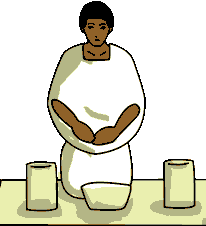
\includegraphics[scale=0.5]{Imagenes/mujer02}}
	\caption{Ciudadanos que se encuentran.}
	\label{fig:Ciudadanos}
\end{figure} 
\subsection{Concepto:}
Los ciudadanos se encuentran para relatar al jugador la época en la que se encuentra, la situación actual que enfrentan, el lugar donde se encuentran y más datos para entender el contexto que lo rodea.
\subsection{Encuentro:}
En el nivel 1.
\subsection{Bloques de animación:}
	\begin{itemize}
		\item Mujer comerciante. 
			\begin{itemize}
				\item Animación mover mercancía de un lado a otro.
			\end{itemize}
		\item Mujer jarrón.
			\begin{itemize}
				\item Animación caminar.
			\end{itemize}			 
		\item Hombre jarrón.
			\begin{itemize}
				\item Animación caminar.
			\end{itemize} 
		\item Hombre cacao.
			\begin{itemize}
				\item Animación caminar.
			\end{itemize}
		\item Hombre noble.
			\begin{itemize}
				\item Animación revisar mercancía(Si esta cerca de un puesto). 
				\item Animación platicar (Si esta cerca de otro noble).
				\item Animación contar granos de cacao (Si no esta cerca de un puesto o de un noble).
			\end{itemize}				
	\end{itemize}	
	\section{Nombre: Quetzalcóatl}  \label{per:quetzalcoatl}
\subsection{Descripción:}
Quetzalcóatl es descrito como un dios blanco y barbado pero nadie lo ha visto después de que decidiera exiliarse.
\subsection{Status:}
NPC 
\subsection{Imagen}
\subsection{Concepto:}
\begin{itemize}
	\item \textbf{Historia antes del juego:}
	Dios que tras perder la batalla de Tula contra Tezcatlipoca decide autoexiliarse. Los dioses que le juraron lealtad cuando se creo el quinto sol esperan su retorno.
	\item \textbf{Historia durante el juego:}
	Al encontrarse exiliado no participa directamente en la historia pero se le ha visto en la caída de Tenochtitlan.
\end{itemize} 
\subsection{Encuentro:}
Se le ve por primera y única vez en la cinemática 1.
\subsection{Habilidades:}
Dios de gran poder capaz de derrotar a Tezcatlipoca si ayuda. Se sabe que ha sido capaz de destruir mundo enteros así como crearlos
\subsection{Armas:}
Sin armas confirmadas.
\subsection{Ítems:}
Se sospecha que tiene en su poder muchas armas de carácter legendario.
	\section{Nombre: Tezcatlipoca}  \label{per:tezcatlipoca}
\subsection{Descripción:}
Tezcatlipoca es el gemelo oscuro de Quetzalcóatl. Usa vestimenta negra. 
\subsection{Status:}
Solo se menciona.
\subsection{Imagen}
Sin imagen. Solo se menciona.
\subsection{Concepto:}
\begin{itemize}
	\item \textbf{Historia antes del juego:}
	Dios causante de la caída de varios de los Soles creados por los dioses. Causó el exilio de Quetzalcóatl para hacerse de más poder dentro de la jerarquía divina. 
	\item \textbf{Historia durante el juego:}
	Es uno de los dioses que gobiernan los trece cielos.
\end{itemize} 
\subsection{Encuentro:}
Únicamente es mencionado por los dioses guardianes.
\subsection{Habilidades:}
Dios de gran poder capaz de derrotar a Quetzalcóatl si ayuda. Se sabe que ha sido capaz de destruir mundo enteros así como crearlos. Se dice que puede conocer el corazón de todos los humanos y dioses. Posee la capacidad de alterar el destino de los humanos a su capricho.
\subsection{Armas:}
Sin armas confirmadas.
\subsection{Ítems:}
Se sospecha que tiene en su poder muchas armas de carácter legendario.
\subsection{Bloques de animación:}
Sin bloques de animación.
	\section{Nombre: Tecolote}   \label{per:tecolote}
\subsection{Descripción:}
Ave perteneciente a la familia de los búhos, de plumaje café y ojos amarillos. Su mirada es profunda. Se encuentra posando sobre una rama seca de árbol rodeado de un destello luminoso. El destello que lo rodea dependerá del nivel en el que se encuentre, permitiéndole siempre resaltar de los demás objetos.
\subsection{Status:}
	\begin{itemize}
		\item Personaje no jugable.
		\item Checkpoint.
	\end{itemize}
\subsection{Imagen}
Ver figura \ref{fig:TecoloteDiseno}
	\begin{figure}
					\centering
					
\includegraphics[height=0.3 \textheight]{Imagenes/armas}
					\caption{Concepto de diseño de Tecolote.}
					\label{fig:TecoloteDiseno}
	\end{figure}
\subsection{Encuentro:}
Todos los niveles.
\subsection{Bloques de animación:}
\begin{itemize}
	\item Animación aleteo de alas.
\end{itemize}
	\section{Nombre: Armadillo}  \label{per:armadillo} 
\subsection{Descripción:}
Armadillo mágico que habita el Mictlán. De color dorado pálido. Su caparazón está cubierto de esmeraldas y cuchillas de obsidiana. Su tamaño es mayor al de un armadillo normal. 
\subsection{Status:}
Enemigo
\subsection{Imagen}
Ver figura \ref{fig:armadillo}
\begin{figure}
	\centering
	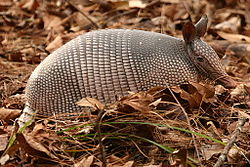
\includegraphics[height=0.2 \textheight]{Imagenes/armadillo}
	\caption{Armadillo.}
	\label{fig:armadillo}
\end{figure} 

\subsection{Encuentro:}
Enemigo del nivel tres del juego (ver apartado \ref{Nivel:Niv03}).
\subsection{Habilidades:}
\begin{itemize}
	\item Cuchillas de obsidiana (ver aparatado \ref{hab.CuchObs}).
\end{itemize}
\subsection{Patrón de ataque:}
El armadillo se moverá en un desplazamiento horizontal del punto A hacia el punto B. Durante su desplazamiento se mostrara su bloque de animación de rodar y cuando llegue a los A o B se activará su habilidad de cuchillas de obsidiana ver aparatado \ref{hab.CuchObs}). 
	\section{Nombre: Fantasma rojo}   \label{per:fantasmaR}
\subsection{Descripción:}
Este enemigo nace de las almas que no quedaron varadas en los niveles del Mictlán al no poder terminar los desafíos. Tiene la forma de un cráneo, en los orificios de los ojos del cráneo se puede ver un brillo espectral. El cráneo está decorado con diferentes patrones de color rojo y verde petróleo en la zona superior del cráneo, la frente, los ojos y la boca. De la parte trasera del cráneo sale fuego cuya paleta de colores es un degradado de rojo y naranja, siendo el rojo el predominante. 
\subsection{Status:}
Enemigo.
\subsection{Imagen}
Ver figura \ref{fig:fantasmaR}.
\begin{figure}
	\centering
	
\includegraphics[height=0.2 \textheight]{Imagenes/fantasmaRojo}
	\caption{Fantasma rojo.}
	\label{fig:fantasmaR}
\end{figure} 
\subsection{Encuentro:}
Enemigo de los niveles 2, 3, 6, 7, 8 y 9. (ver apartados \ref{Nivel:Niv02}, \ref{Nivel:Niv03})
\subsection{Habilidades:}
\begin{itemize}
	\item Disparo rojo. Ver \ref{hab.disparoR}.
\end{itemize}
\subsection{Patrón de ataque:}
El enemigo realizara un recorrido vertical del punto A al B y del B al A de manera cíclica mientras ejecuta la habilidad de disparo rojo.
\subsection{Bloques de animación:}
		\begin{itemize}
			\item Animación fuego.
			\item Animación disparo.
		\end{itemize}
	\section{Nombre: Fantasma morado}   \label{per:fantasmaM}
\subsection{Descripción:}
Alma perdida en el Mictlán. Es un craneo flotate envuelto en una niebla morada.
Se enfrenta al jugador lanzándosele para causarle daño. Si toca al jugador le hace daño. 
\subsection{Status:}
Enemigo.
\subsection{Imagen}
Ver figura \ref{fig:fantasmaM}.
\begin{figure}
	\centering
	
\includegraphics[height=0.2 \textheight]{Imagenes/fantasmaMorado}
	\caption{Fantasma morado.}
	\label{fig:fantasmaM}
\end{figure}
\subsection{Encuentro:}
En niveles 2, 4, 5, 7, 9.
\subsection{Habilidades:}
\begin{itemize}
	\item Embestida. Ver habilidad \ref{hab.embestida}.
	\item Flotar en triángulo. Ver habilidad \ref{hab.flotarT}.
\end{itemize}
\subsection{Patrón de ataque:}
En un ciclo, realizará la habilidad embestida una vez y después la habilidad flotar en triángulo una vez. Este ciclo se repetirá hasta que el enemigo desaparezca.
	\section{Nombre: Jaguar}   \label{per:jaguar}
\subsection{Descripción:}
Felino de color amarillo con manchas negras. A pesar de ser un ser de propiedades mágicas, posee la apariencia de un jaguar común; sin embargo, posee un tamaño y una fuerza superior a éste.
\subsection{Status:}
NPC, enemigo.
\subsection{Imagen}
Ver figura \ref{fig:jaguar}.
\begin{figure}
	\centering
	
\includegraphics[height=0.2 \textheight]{Imagenes/jaguar}
	\caption{Jaguar.}
	\label{fig:jaguar}
\end{figure}
\subsection{Encuentro:}
En el nivel 8 (ver apartado \ref{Nivel:Niv08}).
\subsection{Habilidades:}
\begin{itemize}
	\item Embestida (ver apartado \ref{hab.embestida}).
\end{itemize}
\subsection{Patrón de ataque:}
El enemigo se desplazara del punto A al B utilizando la habilidad de embestida, permanecerá en el punto B por unos segundos .
\subsection{Bloques de animación:}
	\begin{itemize}
		\item Animación embestida.
		\item Animación caminar.
	\end{itemize}
	\section{Nombre: Zopilote}   \label{per:zopilote}
\subsection{Descripción:}
Ave de tamaño mediano. Su plumaje es negro, su cuerpo presenta fisuras de donde se puede ver sus huesos y tonalli corrupto. Su cabeza es calva. No tiene ojos, de las aberturas de sus ojos sale tonalli corrupto. 
\subsection{Status:}
\begin{itemize}
	\item Enemigo normal.
\end{itemize}
\subsection{Imagen}
Ver figura \ref{fig:zopilote}.
\begin{figure}
	\centering
	
\includegraphics[height=0.2 \textheight]{Imagenes/zopilote}
	\caption{Zopilote.}
	\label{fig:zopilote}
\end{figure}
\subsection{Encuentro:}
En el nivel 6 (ver apartado \ref{Nivel:Niv06}).
\subsection{Habilidades:}
\begin{itemize}
	\item Vuelo en picada (ver apartado \ref{hab.Vpicada}).
\end{itemize}
\subsection{Patrón de ataque:}
Su movimiento se da en dos puntos horizontales: A y B. Realiza un patrullaje de punto A al B y del B al A, cada vez que regresa a alguno de los puntos por segunda vez consecutiva ejecuta la habilidad de vuelo en picada (ver apartado \ref{hab.Vpicada}).
\subsection{Bloques de animación:}
\begin{itemize}
		\item Animación vuelo.
		\item Animación caída en picada.
	\end{itemize}

	\section{Nombre: Chara enana}   \label{per:chara}
\subsection{Descripción:}
Ave mágica que habita el Mictlán. Su cuerpo de presenta ligeras llagas de donde salen estalagmitas, estas llagas se pueden ver principalmente en su espalada y cráneo. Su plumaje es de color azul oscuro. 
\subsection{Status:}
NPC, enemigo.
\subsection{Imagen}

%\begin{figure}
%	\centering
%	
\includegraphics[height=0.2 \textheight]{Imagenes/jaguar}
%	\caption{Jaguar.}
%	\label{fig:jaguar}
%\end{figure}
\subsection{Encuentro:}
En el nivel 5 (ver apartado \ref{Nivel:Niv05}).
\subsection{Habilidades:}
\begin{itemize}
	\item Vuelo en picada (ver apartado \ref{hab.Vpicada}).
\end{itemize}
\subsection{Patrón de ataque:}
Su movimiento se da en dos puntos horizontales: A y B. Realiza un patrullaje de punto A al B y del B al A, cada vez que regresa a alguno de los puntos por segunda vez consecutiva ejecuta la habilidad de vuelo en picada (ver apartado \ref{hab.Vpicada}).
	
	\chapter{Obstáculos}
	\section{Nombre: Caja} \label{obs.caja}
\subsection{Descripción}
Caja de madera. Es inamovible e indestructible. El jugador deberá saltarla para superarla. 
\subsection{Esquema}
Ver figura \ref{fig:caja}.
\begin{figure}
	\centering
	
\includegraphics[height=0.1 \textheight]{Imagenes/caja}
	\caption{Caja de madera.}
	\label{fig:caja}
\end{figure}	
	\section{Nombre: Sacos cacao}\label{obs.saco}
\subsection{Descripción}
Conjunto de seis sacos de cacao apilados en tres niveles, el primer nivel tendra tres sacos, el segundo nivel dos y por último solo uno. Tiene dos comportamientos:
\begin{itemize}
	\item Como objeto de fondo, en donde le jugador podrá pasarlo de largo sin ningún tipo de interacción. 
	\item Como obstáculo, en donde es inamovible e indestructible. El jugador deberá saltarla para superarla.
\end{itemize}
\subsection{Esquema}
Ver figura \ref{fig:saco}.
\begin{figure}
	\centering
	
\includegraphics[height=0.2 \textheight]{Imagenes/saco}
	\caption{Sacos de cacao.}
	\label{fig:saco}
\end{figure}
	\section{Nombre: Plataforma móvil}\label{obs.plataformaM}
	\subsection{Descripción}
Porción de suelo que describe un movimiento del punto A al B y del B al A. La posición de estos puntos varia dependiendo del nivel, logrando que este objeto tenga un desplazamiento vertical, horizontal o en diagonal. El jugador deberá saltar sobre este obstáculo utilizando el desplazamiento de la plataforma para avanzar.
	\subsection{Esquema}
	Ver figura \ref{fig:plataformaM}.
	\begin{figure}
		\centering
		
\includegraphics[height=0.2 \textheight]{Imagenes/plataformaM}
		\caption{Plataforma móvil.}
		\label{fig:plataformaM}
	\end{figure}
	\section{Nombre: Plataforma que cae.}\label{obs.plataformaD}
	\subsection{Descripción}
	Porción de suelo que cae después de n cantidad de segundos que el jugador ha aterrizado sobre ella.
	\subsection{Esquema}

	\section{Nombre: Rocas}\label{obs.rocas}
	\subsection{Descripción}
	Conjunto de piedras o rocas posicionadas en un punto determinado, preferentemente alto. Este objeto cuenta con un área donde se detecta si ha pasado el jugador, de ser así las piedras caerán.
	\subsection{Esquema}
	Ver figura \ref{fig:rocas}.
	\begin{figure}
		\centering
		
\includegraphics[height=0.2 \textheight]{Imagenes/rocas}
		\caption{Rocas cayendo cuando el jugador ha paso por el área.}
		\label{fig:rocas}
	\end{figure}
			\section{Nombre: Viento temporal}\label{obs.vientoT}
	\subsection{Descripción}
	Ráfaga de viento. Impulsa al jugador de manera horizontal, dependiendo del nivel lo empujara hacia la izquierda o hacia la derecha. Su efecto no es constante, se activa y desactiva de manera periódica estando activo durante un tiempo determinado y desactivándose por otro tiempo determinado; los tiempos de actividad e inactividad pueden no ser los mismos. Para superar este obstáculo el jugador deberá aprovechar los tiempos de inactividad y cruzar la zona donde aparece la ráfaga.
	\subsection{Esquema}

			\section{Nombre: Piedras filosas}\label{obs.piedrasF}
	\subsection{Descripción}
	Piedra de gran tamaño. Es inamovible e indestructible. Cuando el jugador hace contacto con este objeto se reduce su cantidad de vida. Para superarla el jugador debe de saltar sobre ella evitando hacer contacto.
	\subsection{Esquema}
Ver figura \ref{fig:Piedras}.
\begin{figure}
	\centering
	
\includegraphics[height=0.1 \textheight]{Imagenes/piedras01}
	\caption{Piedras filosas.}
	\label{fig:Piedras}
\end{figure}
		\section{Nombre: Piso congelado}\label{obs.pisoC}
	\subsection{Descripción}
	Porción de suelo. Cuando el jugador camina sobre este obstáculo, la fricción entre el jugador y el obstáculo disminuye provocando que la velocidad de desplazamiento del jugador se incremente y que cuando el jugador se detenga no lo haga de golpe sino resbale una distancia determinada antes de detenerse.
	\subsection{Esquema}
	Ver figura \ref{fig:pisoC}.
	\begin{figure}
		\centering
		
\includegraphics[height=0.2 \textheight]{Imagenes/pisoC}
		\caption{Piso congelado.}
		\label{fig:pisoC}
	\end{figure}
			\section{Nombre: Hielo quebradizo}\label{obs.hieloQ}
	\subsection{Descripción}
	Pedazo de terreno, consta de hielo fracturado visualmente, es rígido. Al contacto con el jugador después de unos segundos empieza a desaparecer, reaparece luego de otros segundos más.
	\subsection{Esquema}
	Ver figura \ref{fig:hieloQ}.
	\begin{figure}
		\centering
		
\includegraphics[height=0.2 \textheight]{Imagenes/hieloQ}
		\caption{Hielo quebradizo y como se rompe cuando el jugador se para en cima.}
		\label{fig:hieloQ}
	\end{figure}
			\section{Nombre: Bolas de nieve}\label{obs.bolasN}
	\subsection{Descripción}
	Conjunto de bolas de nieve, su característica es rígida. Posicionadas en un punto determinado, preferentemente alto. Este objeto cuenta con un área donde se detecta si ha pasado el jugador, de ser así las bolas de nieve caerán.
	\subsection{Esquema}
	Ver figura \ref{fig:bolasN}.
	\begin{figure}
		\centering
		
\includegraphics[height=0.2 \textheight]{Imagenes/bolasN}
		\caption{Sacos de cacao.}
		\label{fig:bolasN}
	\end{figure}
		\section{Nombre: Viento multidireccional}\label{obs.vientoM}
	\subsection{Descripción}
		Ráfaga de viento, este objeto no es rígido y puede ser visible solo por las animaciones ocasionales de líneas rectas (horizontales, verticales, diagonales). El viento se activa por lapsos de tiempo constantes. El jugador al entrar en contacto con el viento le estará dando una velocidad constante en una dirección aleatoria que podría ser horizontal, vertical o en diagonal, provocando un "empuje" del personaje. 
	\subsection{Esquema}
	Ver figura \ref{fig:vientoM}.
	\begin{figure}
		\centering
		
\includegraphics[height=0.2 \textheight]{Imagenes/vientoM}
		\caption{Sacos de cacao.}
		\label{fig:vientoM}
	\end{figure}
			\section{Nombre: Lluvia de flechas}\label{obs.lluviaF}
	\subsection{Descripción}
	Consiste en flechas cayendo aleatoriamente sobre el eje horizontal hacia el piso y constantemente. Al contacto con el jugador le resta puntos de vida.
	\subsection{Esquema}
	Ver figura \ref{fig:lluviaF}.
	\begin{figure}
		\centering
		
\includegraphics[height=0.2 \textheight]{Imagenes/lluviaF}
		\caption{Lluvia de flechas representada en un nivel.}
		\label{fig:lluviaF}
	\end{figure}
	\chapter{Habilidades.}
%=============================================================
	\section{Cuchillas de obsidiana} \label{hab.CuchObs}	
		\subsection{Descripción}
		El enemigo lanza pequeños círculos rojos en dirección horizontal que dañan al jugador. Los disparos salen de la parte frontal del enemigo.
		\subsection{Portador}
		Armadillo (ver apartado \ref{per:armadillo})
		\subsection{Esquema}

%============================================================
		\section{Nombre: Disparo rojo.} \label{hab.disparoR}
		\subsubsection{Descripción}
		El enemigo lanza pequeños círculos rojos en dirección horizontal que dañan al jugador. Los disparos salen de la parte frontal del enemigo.
		\subsubsection{Portador}
		Fantasma rojo. Ver \ref{per.fantasmaR}.
		\subsubsection{Esquema}
		Ver figura \ref{fig:disparoR}.
		\begin{figure}
			\centering
			
\includegraphics[height=0.2 \textheight]{Imagenes/disparoR}
			\caption{Disparo rojo.}
			\label{fig:disparoR}
		\end{figure}
			%============================================================
	\section{Nombre: Embestida.} \label{hab.embestida}
		\subsection{Descripción}
		El enemigo aumenta su velocidad mientras se desplaza de arriba hacia abajo en diagonal.
		\subsection{Portador}
		Fantasma morado. Ver \ref{per.fantasmaM}.
		\subsection{Esquema}
		Ver figura \ref{fig:embestida}.
		\begin{figure}
			\centering
			
\includegraphics[height=0.2 \textheight]{Imagenes/embestida}
			\caption{Embestida.}
			\label{fig:embestida}
		\end{figure}

%============================================================
	\section{Nombre: Rapto.} \label{hab.rapto}
		\subsection{Descripción}
		El enemigo se mueve hacia la posición del jugador, lanzándose de su posición hacia abajo con una desviación curva.
		\subsection{Portador}
		Zopilote. Ver \ref{per.zopilote}.
		\subsection{Esquema}
		Ver figura \ref{fig:rapto}.
		\begin{figure}
			\centering
			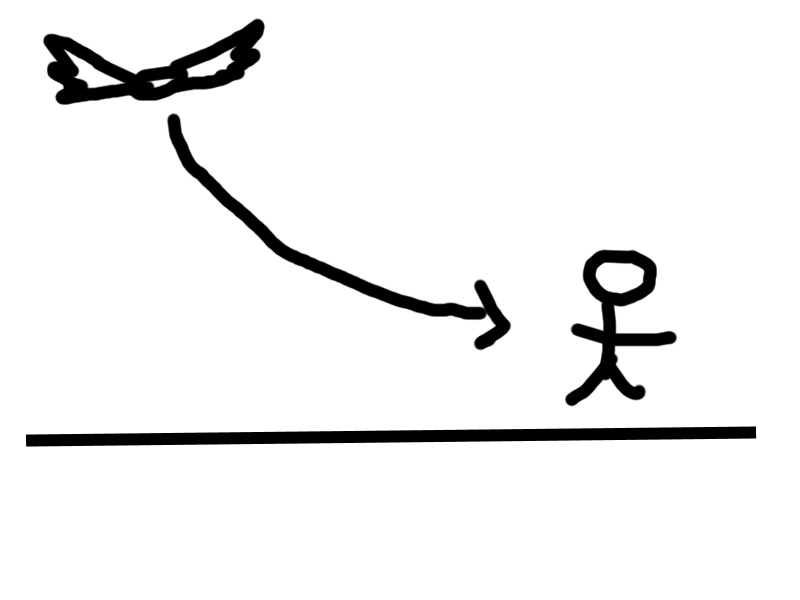
\includegraphics[height=0.2 \textheight]{Imagenes/rapto}
			\caption{Zopilote.}
			\label{fig:rapto}
		\end{figure}

%============================================================
	\section{Nombre: Zopilotear.} \label{hab.zopilotear}
		\subsection{Descripción}
		El enemigo se mueve de manera circular por sobre el piso.
		\subsection{Portador}
		Zopilote. Ver \ref{per.zopilote}.
		\subsection{Esquema}
		Ver figura \ref{fig:zopilotear}.
		\begin{figure}
			\centering
			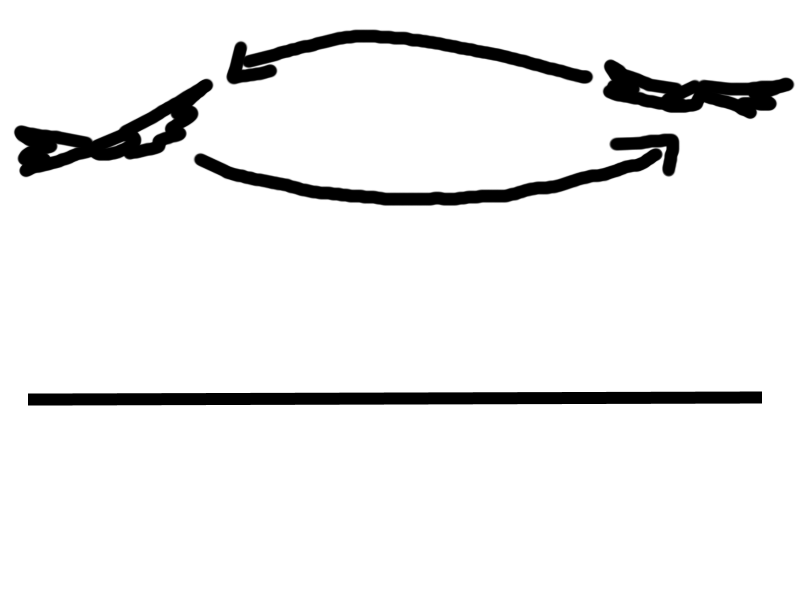
\includegraphics[height=0.2 \textheight]{Imagenes/zopilotear}
			\caption{Zopilotear.}
			\label{fig:zopilotear}
		\end{figure}

%============================================================
			\section{Nombre: Embestida.} \label{hab.embestida}
			\subsection{Descripción}
			El enemigo con sus garras ataca al jugador.
			\subsection{Portador}
			Jaguar. Ver \ref{per.jaguar}.
			\subsection{Esquema}
			Ver figura \ref{fig:zarpazo}.
			\begin{figure}
				\centering
				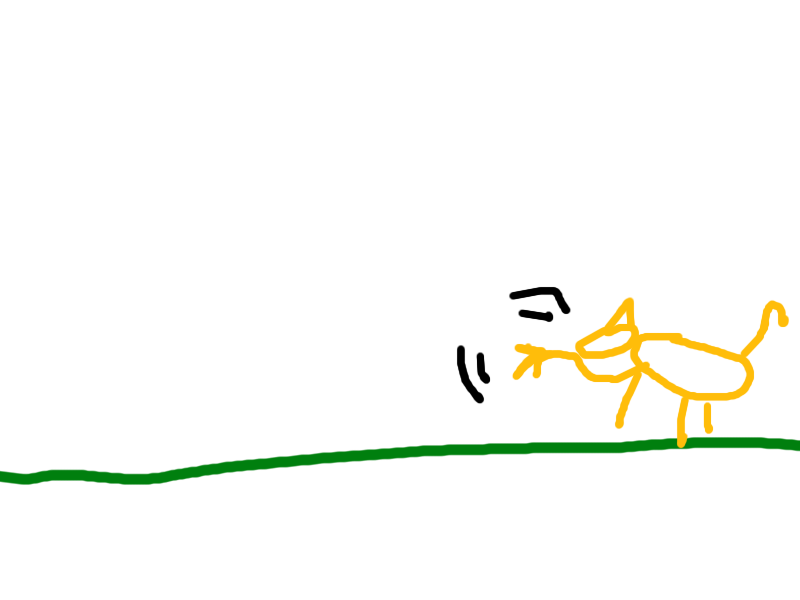
\includegraphics[height=0.2 \textheight]{Imagenes/zarpazo}
				\caption{Zarpazo.}
				\label{fig:zarpazo}
			\end{figure}
			
			%============================================================
\section{Nombre: Disparo de tonalli.}\label{hab.disparoT}
\subsection{Descripción}
Con ayuda de la caracola permite a su portador disparar tonalli.
\subsection{Portador}
Malinalli
\subsection{Esquema}
			Ver figura \ref{fig:disparoT}.
			\begin{figure}
				\centering
				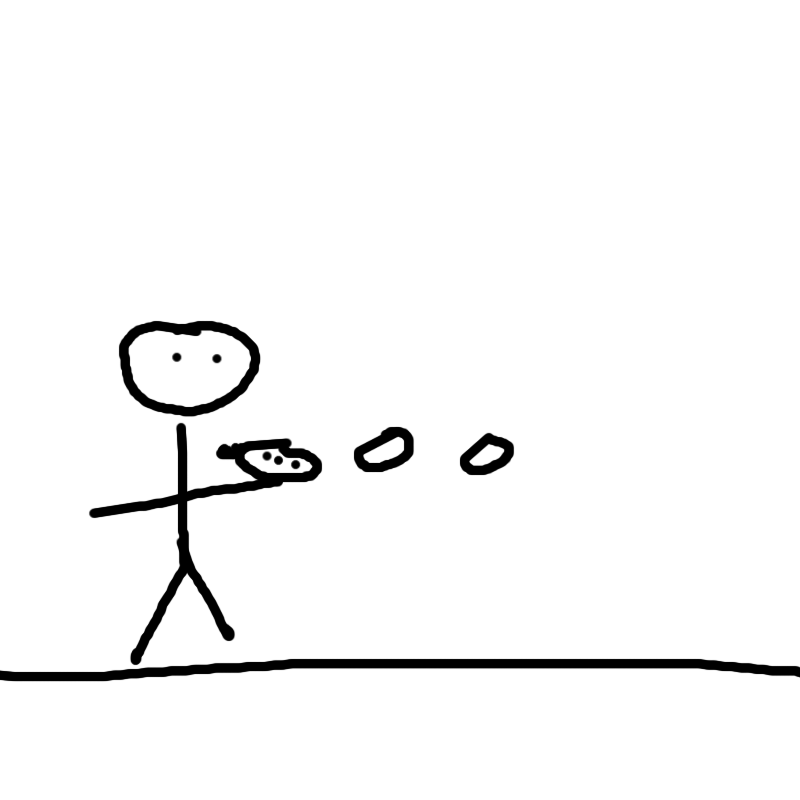
\includegraphics[height=0.2 \textheight]{Imagenes/disparoT}
				\caption{Disparo de tonalli por el jugador.}
				\label{fig:disparoT}
			\end{figure}
			
%============================================================
\section{Nombre: Zambullida.}\label{hab.zambullida}
\subsection{Descripción}
Zochitónal se sumerge en el río, dejando solo en la superficie parte de su espalda; procediendo a nadar a gran velocidad de un lado a otro para embestir a sus enemigos.  
\subsection{Portador}
Zochitónal
\subsection{Esquema}
			Ver figura \ref{fig:zambullida}.
			\begin{figure}
				\centering
				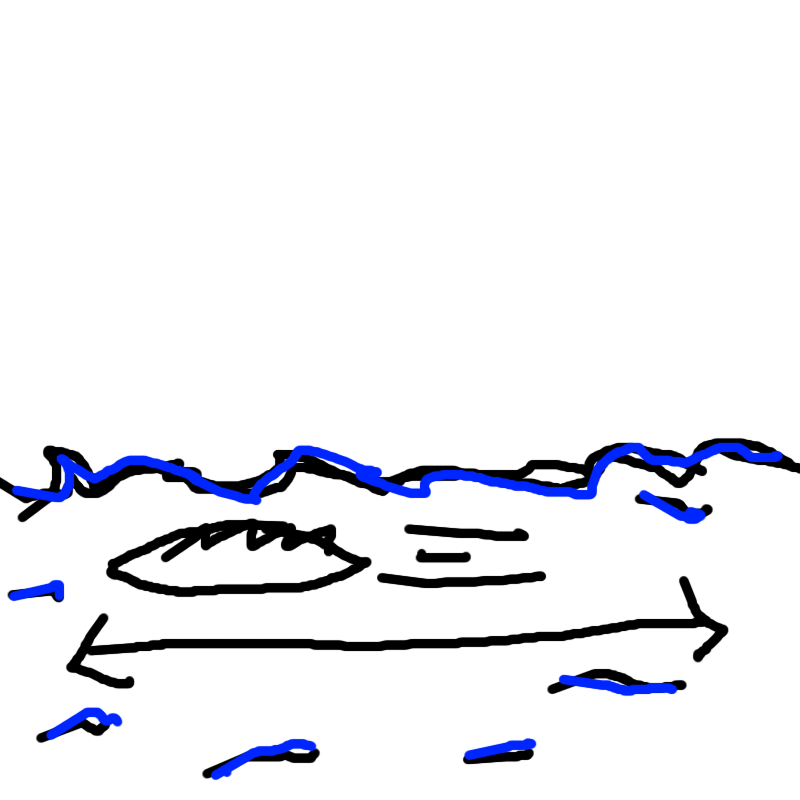
\includegraphics[height=0.2 \textheight]{Imagenes/zambullida}
				\caption{Zambullida.}
				\label{fig:zambullida}
			\end{figure}
%============================================================
\section{Nombre: Burbujas.}\label{hab.burbujas}
\subsection{Descripción}
Zochitónal dispara burbujas que seguirán al jugador por un tiempo.  
\subsection{Portador}
Zochitónal
\subsection{Esquema}
			Ver figura \ref{fig:burbujas}.
			\begin{figure}
				\centering
				
\includegraphics[height=0.2 \textheight]{Imagenes/burbujas}
				\caption{Burbujas.}
				\label{fig:burbujas}
			\end{figure}

%============================================================
\section{Nombre: Coraza.}\label{hab.coraza}
\subsection{Descripción}
Esta habilidad permite crear una coraza de piedra protegiendo a su portador de ataques enemigos sacrificando velocidad de movimiento.  
\subsection{Portador}
Tepeyóllotl.
\subsection{Esquema}
			Ver figura \ref{fig:coraza}.
			\begin{figure}
				\centering
				\includegraphics[height=0.2 \textheight]{Imagenes/coraza}
				\caption{Coraza.}
				\label{fig:coraza}
			\end{figure}
%============================================================
\section{Nombre: Impacto.} \label{hab.impacto}
\subsection{Descripción}
Realiza un salto, provocando al aterrizaje una onda de piedras en el suelo.
\subsection{Portador}
Tepeyóllotl.
\subsection{Esquema}

%============================================================
\section{Nombre de la habilidad: Luvia de rocas.} \label{hab.LLuviaRocas}
\subsection{Descripción}
Con un poderoso rugido provoca una avalancha de rocas. 
\subsection{Portador}
Tepeyóllotl.
\subsection{Esquema}
			Ver figura \ref{fig:lluviaR}.
			\begin{figure}
				\centering
				\includegraphics[height=0.2 \textheight]{Imagenes/lluviaR}
				\caption{Lluvia de rocas.}
				\label{fig:lluviaR}
			\end{figure}
			
%============================================================
\section{Nombre: Rugido aturdidor.}\label{hab.RugAtur}
\subsection{Descripción}
Poderoso rugido provoca una de continuo echo que inmoviliza a al enemigo, Tepeyóllotl solo puede usar esta habilidad cuando no usa la coraza. 
\subsection{Portador}
Tepeyóllotl. 
\subsection{Esquema}
			Ver figura \ref{fig:rugido}.
			\begin{figure}
				\centering
				\includegraphics[height=0.2 \textheight]{Imagenes/rugido}
				\caption{Rugido aturdidor.}
				\label{fig:rugido}
			\end{figure}
			
%============================================================
\section{Nombre: Circulo de fuego.} \label{hab.CirFue}
\subsection{Descripción}
Itzpápalotl se eleva en el aire y se rodea a sí misma con fuego, este ataque sera usado cuando el jugador se encuentre junto a ella.
\subsection{Portador}
Itzpápalotl. 
\subsection{Esquema}
			Ver figura \ref{fig:circuloF}.
			\begin{figure}
				\centering
				\includegraphics[height=0.2 \textheight]{Imagenes/circuloF}
				\caption{Círculo de fuego.}
				\label{fig:circuloF}
			\end{figure}
			
%============================================================
\section{Nombre: Embestida aerea.}\label{hab.EmbesAer}
\subsection{Descripción}
Itzpápalotl usara este ataque cuando este lejos del jugador. Itzpápalotl saltar y en el aire se lanza contra el enemigo en diagonal.
\subsection{Portador}
Itzpápalotl.
\subsection{Esquema}
			Ver figura \ref{fig:embestidaA}.
			\begin{figure}
				\centering
				\includegraphics[height=0.2 \textheight]{Imagenes/embestidaA}
				\caption{Embestida aerea.}
				\label{fig:embestidaA}
			\end{figure}
%============================================================
\section{Nombre: Invisibilidad.} \label{hab.Invis}
\subsection{Descripción}
Esta habilidad le permite ser indetectable al ojo de dioses y humanos, permitiendole tomar una posición ventajosa en combate.
\subsection{Portador}
Itzpápalotl.
\subsection{Esquema}
			Ver figura \ref{fig:invisibilidad}.
			\begin{figure}
				\centering
				\includegraphics[height=0.2 \textheight]{Imagenes/invisibilidad}
				\caption{Invisibilidad.}
				\label{fig:invisibilidad}
			\end{figure}
%============================================================
\section{Nombre: Tornado.} \label{hab.tornado}
\subsection{Descripción}
Poderoso ataque que puede bajar hasta la mitad de la vida del jugador.
\subsection{Portador}
Mictlecayotl.
\subsection{Esquema}
			Ver figura \ref{fig:tornado}.
			\begin{figure}
				\centering
				\includegraphics[height=0.2 \textheight]{Imagenes/tornado}
				\caption{Tornado.}
				\label{fig:tornado}
			\end{figure}

%============================================================
\section{Nombre: Ventisca.} \label{ventisca}
\subsection{Descripción}
Aire helado que puede causar una pérdida considerable de la barra de salud.
\subsection{Portador}
Mictlecayotl.
\subsection{Esquema}
			Ver figura \ref{fig:ventisca}.
			\begin{figure}
				\centering
				\includegraphics[height=0.2 \textheight]{Imagenes/ventisca}
				\caption{Ventisca.}
				\label{fig:ventisca}
			\end{figure}

%============================================================
\section{Nombre: Raíz del diablo.}\label{hab.RaizDia}
\subsection{Descripción}
Ataque que produce una confusión en el jugador, haciendo que los botones no reaccionen con las acciones que deberían.
\subsection{Portador}
Tlazoltéotl.
\subsection{Esquema}
			Ver figura \ref{fig:raiz}.
			\begin{figure}
				\centering
				\includegraphics[height=0.2 \textheight]{Imagenes/raiz}
				\caption{Raíz del diablo.}
				\label{fig:raiz}
			\end{figure}

%============================================================
\section{Nombre: Energía corrupta.} \label{hab.CorrupEner}
\subsection{Descripción}
Esferas de energia oscura que infringen daño al jugador al hacer contacto con éste.
\subsection{Portador}
Tlazoltéotl.
\subsection{Esquema}
			Ver figura \ref{fig:energiaC}.
			\begin{figure}
				\centering
				\includegraphics[height=0.2 \textheight]{Imagenes/energiaC}
				\caption{Energía corrupta.}
				\label{fig:energiaC}
			\end{figure}	

%============================================================
\section{Nombre: Circulo protector.} \label{hab.CirPro}
\subsection{Descripción}
Utilizando energía corrupta,  Tlazoltéotl crea alrededor de ella un circulo con la capacidad de protegerla contra cualquier ataque.
\subsection{Portador}
Tlazoltéotl.
\subsection{Esquema}
			Ver figura \ref{fig:circuloP}.
			\begin{figure}
				\centering
				\includegraphics[height=0.2 \textheight]{Imagenes/circuloP}
				\caption{Círculo protector.}
				\label{fig:circuloP}
			\end{figure}

%============================================================
\section{Nombre: LLuvia de lava.} \label{hab.LLuviaLava}
\subsection{Descripción}
Caen bolas de lava con una gran capacidad de daño.
\subsection{Portador}
Itztlacoliuhqui.	
\subsection{Esquema}	
			Ver figura \ref{fig:lluviaL}.
			\begin{figure}
				\centering
				\includegraphics[height=0.2 \textheight]{Imagenes/lluviaL}
				\caption{Lluvia de lava.}
				\label{fig:lluviaL}
			\end{figure}

%============================================================
\section{Nombre: Manotazo.} \label{hab.Manotazo}
\subsection{Descripción}
Genera una onda expansiva que deforma el suelo provonado una oleada de rocas.
\subsection{Portador}
\subsection{Esquema}
			Ver figura \ref{fig:manotazo}.
			\begin{figure}
				\centering
				\includegraphics[height=0.2 \textheight]{Imagenes/manotazo}
				\caption{Manotazo.}
				\label{fig:manotazo}
			\end{figure}
Itztlacoliuhqui.

%============================================================
\section{Nombre: Lluvia de flechas.} \label{hab.LluviaFle}
\subsection{Descripción}
Como su nombre lo dice, provoca una lluvia de flechas, este es el ataque de Itztlacoliuhqui que genera el menor nivel de daño. 
\subsection{Portador}
Itztlacoliuhqui.
\subsection{Esquema}
			Ver figura \ref{fig:lluviaF}.

%============================================================
\section{Nombre: Todos los hombres del rey.}\label{hab.TodoRey}
\subsection{Descripción}
Con este ataque,  Mictlantechtli invoca a varios de los enemigos normales que habitan el Mictlán para que se enfrenten al jugador mientras  Mictlantechhtli desaparece.
\subsection{Portador}
Mictlantechtli.
\subsection{Esquema}
			Ver figura \ref{fig:rey}.
			\begin{figure}
				\centering
				\includegraphics[height=0.2 \textheight]{Imagenes/rey}
				\caption{Todos los hombres del rey.}
				\label{fig:rey}
			\end{figure}
%============================================================
\section{Nombre: Fuego mortífero.} \label{hab.FuegoMor}
\subsection{Descripción}
Mictlantechtli  lanza poderosas esferas de fuego verde.
\subsection{Portador}
Mictlantechtli.	
\subsection{Esquema}	
			Ver figura \ref{fig:fuegoM}.
			\begin{figure}
				\centering
				\includegraphics[height=0.2 \textheight]{Imagenes/fuegoM}
				\caption{fuegoM.}
				\label{fig:fuegoM}
			\end{figure}
%============================================================
\section{Nombre: Penitencia.}\label{hab.Penitencia}
\subsection{Descripción}
Mictlantechtli se eleva en el aire haciendo que salgan huesos filosos del suelo.
\subsection{Portador}
Mictlantechtli.
\subsection{Esquema}
			Ver figura \ref{fig:penitencia}.
			\begin{figure}
				\centering
				\includegraphics[height=0.2 \textheight]{Imagenes/penitencia}
				\caption{Penitencia.}
				\label{fig:penitencia}
			\end{figure}

%============================================================
\section{Nombre: Lluvia de huesos.}\label{hab.LluHuesos}
\subsection{Descripción}
Se invocan afilados huesos que caen del cielo. Este  elevado nivel de daño al jugador.
\subsection{Portador}
Mictlantechtli.
\subsection{Esquema}
			Ver figura \ref{fig:penitencia}.
			\begin{figure}
				\centering
				\includegraphics[height=0.2 \textheight]{Imagenes/penitencia}
				\caption{Penitencia.}
				\label{fig:penitencia}
			\end{figure}
			
%============================================================
\section{Nombre: Estocada mortífera..}\label{hab.estMor}
\subsection{Descripción}
Se invoca un solo hueso gigante que recorre el campo de manera horizontal a la altura del suelo con gran velocidad. Este ataque puede generar gran daño.
\subsection{Portador}
Mictlantechtli.
\subsection{Esquema}
			Ver figura \ref{fig:penitencia}.
			\begin{figure}
				\centering
				\includegraphics[height=0.2 \textheight]{Imagenes/penitencia}
				\caption{Penitencia.}
				\label{fig:penitencia}
			\end{figure}			
			
 	\chapter{Armas.}
\section{Nombre: Caracola.} \label{Arma:Caracola}
\subsection{Descripción}
Esta arma con forma de cenzontle contiene el alma de uno dentro, lo que le permita generar todo tipo de sonidos. El sonido que produce se ve materializado como energía luminosa que puede atacar a los enemigos y proteger a su portador al generar una barrera.
\subsection{Imagen}
\subsection{Portador}
Malinalli.

\section{Nombre: Atardecer de venus.}\label{Arma:BaculoXolotl}
\subsection{Descripción}
Báculo que permite amplificar la magia de quien lo porta. Xólotl solamente puede utilizarlo en su forma humana.
\subsection{Imagen}
\subsection{Portador}
Xólotl.

\section{Nombre: Matlalpapalotl.}\label{Arma:LanzaItzpapalotl}
\subsection{Descripción}
Tepoztopilli hecho de obsidiana. Arma creada por Iztpapalotl a partir de las almas de los enemigos derrotados durante la guerra contra los dioses del norte. Es un arma de gran poder, es ligera, ideal para el combate aéreo.
\subsection{Imagen}
\subsection{Portador}
Itzpápalotl.

\section{Nombre: Trepa viento.}\label{Arma:EspadaMictlecayotl}
\subsection{Descripción}
Macuahuitl creada por Mictlecayotl para canalizar su energía de viento y generar poderoso ataques.
\subsection{Imagen}
\subsection{Portador}
Macuahuitl.

\section{Nombre: Arco solar.}\label{Arma:ArcoItztla}
\subsection{Descripción}
Arma legendaria que Itztlacoliuhqui usaba desde antes del quinto Sol, siendo éste el único objeto que se le permiti conservar de su antigua identidad. Es un arco de gran alcance, permite disparar flechas con la capacidad de destruir mundos enteros. 
\subsection{Imagen}
\subsection{Portador}
Itztlacoliuhqui.
	\chapter{Items.}
	\subsection{Nombre: Peineta en forma de flor.}\label{item:peineta}
	\subsection{Descripción}
	Fue un regalo de su padre cuando niña, Malinalli la considera su mayor tesoro.
	\subsection{Imagen}
	\subsection{Portador}
	Malinalli 

	\section{Nombre: Armadura espiritual.}\label{item:armadura}
	\subsection{Descripción}
	Cubre todo el cuerpo de Malinalli, pero visualmente adopta una forma que ella desee.
	\subsection{Imagen}
	\subsection{Portador}
	Malinalli 
	
	\section{Nombre: Flor de vainilla.}\label{item:vainilla}
	\subsection{Descripción}
	
	\subsection{Imagen}
	\subsection{Portador}
	Malinalli 
	
	\section{Nombre: Grano de cacao.}\label{item:cacao}
	\subsection{Descripción}
	
	\subsection{Imagen}
	\subsection{Portador}
	Malinalli 
	
	\section{Nombre: Xoloitzcuintle.}\label{item:Xolo}
	\subsection{Descripción}
	
	\subsection{Imagen}
	\subsection{Portador}
	Sin portador. 
	
	\section{Mariposa} \label{item:Mariposa}
		\subsection{}
		Mariposa azul de tamaño normal. Se encontrara en diferentes puntos del mapa del nivel 4 (ver apartado \ref{Nivel:Niv04})  para indicarle al jugador que esta siguiendo el camino correcto al templo de Itzpapálotl.
	\chapter{Guión}
	\section{Cinemática 1. Afueras de Tenochtitlan. exterior / tarde.} \label{Cin:Cinematica01}
	
\textsc{Personajes}:
\begin{itemize}
	\item Quetzalcóatl (Forma human).
	\item Xólotl (Forma human).
\end{itemize}
\textit{El viento sopla, Quetzalcóatl (en su forma humana) está sentado, viendo en dirección de la ciudad. La ciudad Tenochtitlan se ve parcialmente destruida, de ella sale humo. Entra Xólotl (En su forma humana)}.
\begin{center}
\textsc{\underline{Xólotl}}
\par
De todos los lugares y personas posibles, jamás creí que te encontraría precisamente a ti en este lugar.
\par
\textit{(Quetzalcóatl sigue observando la ciudad en silencio)}
\par
Así es como serán las cosas.
\par 
\textit{(Quetzalcóatl continua en silencio, Xólotl se molesta)}
\par
¿Guardaras silencio para siempre? ¿Ese es el modo en que me castigaras por lo que he hecho?
\\
\par
\textsc{\underline{Quetzalcóatl}}
\par
La caída del quinto sol. ¿Quién lo hubiera creído? Todo cuanto conocimos está por cambiar o desaparecer.
\par
\par
\textsc{\underline{Xólotl}}
\\
\par
Jamás debiste irte. Las cosas habrían sido diferentes si nos hubieras guiado.
\\
\par
\textsc{\underline{Quetzalcóatl}}
\par
Te equivocas. Las cosas son como tenían que ser. Dime… ¿Valió la pena? El duro viaje y las batallas. ¿Todo eso te dio lo que tanto anhelabas?
\\
\par
\textsc{\underline{Xólotl}}
\\
\par
\textit{(Guarda silencio por un momento)}
\\
\par
No …
\end{center}
	\section{Cinemática 2. Mercado de Centla. Exterior /día.} \label{Cin:Cinematica02}
\textsc{Personajes}:
\begin{itemize}
	\item Malinalli Tenelpan.
	\item Xólotl (Forma xoloitzcuintle).
\end{itemize}

\textit{Malinalli(15 años) está parada cuando Xólotl le roba un objeto.}
\begin{center}
\textsc{\underline{malinalli}}
\\
\par
Mi amo me va a matar. El xoloitzcuintle ha tomado el mensaje que el amo le enviaba a su amada. Tengo que alcanzarlo y recuperar el mensaje. (\textit{Sale corriendo}).
\end{center}
	\section{Cinemática 3. Selva a las afueras de Centla. Exterior /día.} \label{Cin:Cinematica03}
\textsc{Personajes}:
\begin{itemize}
	\item Malinalli Tenelpan.
	\item Xólotl (Forma xoloitzcuintle).
\end{itemize}
\textit{Después de buscar a Xólotl por la selva, Malinalli cae de una colina.}
\begin{center}
	\textsc{\underline{malinalli}}
	\\	
	\par
Eso ha dolido bastante.
(Escucha ruido proveniente de los arbustos, trata de reincorporase. Xólotl sale de los arbustos. Malinalli trata de retroceder, pero se da cuenta de que está atrapada. Xólotl se acerca a ella. Malinalli se queda quieta, cuando el jaguar está muy cerca lo toca en el rostro viéndolo a los ojos tratando de controlar su miedo. Xólotl la mira y se transforma en un xoloitzcuintle)
\\	
	\par
\textsc{\underline{Xólotl}}
\\	
	\par
Hola, Malinalli. Llevo casi una eternidad buscando a alguien como tú.
(Malinalli retrocede, tratando de protegerse)
Tranquila no pienso lastimarte.
(Malinalli sigue tratando de escapar, Xólotl la congela para que lo escuche usando su poder para acercarla a él).
Si quisiera asesinarte ya lo hubiera hecho.
\\	
	\par
\textsc{\underline{malinalli}}
\\	
	\par
Suéltame. Déjame ir. No tengo nada que pueda serte útil.
\\	
	\par
\textsc{\underline{Xólotl}}
\\	
	\par
Todo lo contrario. Tienes exactamente lo que necesito. He oído muchas cosas de ti. Malinalli Tenelpan, la joven de origen noble que ahora es esclava. Al igual que tu pertenecí a lo más alto de mi mundo.
\\	
	\par
\textsc{\underline{malinalli}}
\\	
	\par
¿Qué eres?
\\	
	\par
\textsc{\underline{Xólotl}}
\\	
	\par
Soy Xólotl. Un dios que vino a responder a tus plegarias.
\\	
	\par
\textsc{\underline{malinalli}}
\\	
	\par
¿Porqué un dios atendería las plegarias de una insignificante esclava?
\\	
	\par
\textsc{\underline{Xólotl}}
\\	
	\par
Porque la esclava tiene lo que muchos hombres nobles y de alta cuna carecen: Valentia. 
\\	
	\par
\textsc{\underline{malinalli}}
\\	
	\par
Agradezco sus palabras, pero me temo que se equivoca. Soy solo una esclava, nada más.
\\	
	\par
\textsc{\underline{Xólotl}}
\\	
	\par
El mundo espiritual ha sido tomado por la tiranía de los cuatro hermanos. Toda divinidad que no se acate a sus deseos ha sido destruida o exiliada. El caos gobierna a los dioses. Mi objetivo es liberarlos. Pero no tengo el poder suficiente como para hacerle frente a gobernante supremo de los dioses: Tezcatlipoca.
\\	
	\par
\textsc{\underline{malinalli}}
\\	
	\par
Muy noble de su parte. Sin embrago, no puedo ver cómo es que mi presencia se relaciona con tan gran y noble empresa.
\\	
	\par
\textsc{\underline{Xólotl}}
\\	
	\par
Necesito que alguien baje conmigo al Mictlán, me ayude a reclamar el poder de los guardianes del Mictlán y derrote a Mictlantecuhtli.
\\	
	\par
\textsc{\underline{malinalli}}
\\	
	\par
Una misión digna de un guerrero o un sacerdote no de una esclava.
\\	
	\par
\textsc{\underline{Xólotl}}
\\	
	\par
Ciertamente pero ningún guerrero o sacerdote emprendería una batalla contra los dioses que juraron servir. Los humanos sirven fielmente a sus dioses, hacen guerras por ellos, viven y mueren a su nombre, pero los dioses que gobiernan los trece cielos no miran por los desprotegidos, no les importan los mortales. He visto a los mortales de cerca, he visto sus ciudades nacer y caer. He visto su sufrimiento. Por eso puedo decirte que incluso un esclavo puede cambiar el rumbo de la historia si tiene la motivación adecuada.
(Libera a Malinalli de su poder)
Extrañas a tu padre ¿No es así? Con el Mictlán en mi poder, traerlo de vuelta no sería ningún problema. Con la fuerza de tu padre y sus antiguos ejércitos recuperar tu hogar sería una cuestión de días.  
\\	
	\par
\textsc{\underline{malinalli}}
\\	
	\par
¿Es eso posible? ¿Revivir a alguien es posible?
\\	
	\par
\textsc{\underline{Xólotl}}
\\	
	\par
Con mi poder actual no, pero con el poder de Mictlantecuhtli y los guardianes del inframundo, podre hacer eso y más. ¿Significa que tenemos un trato?
\\	
	\par
\textsc{\underline{malinalli}}
\\	
	\par
¿Cómo destruiré a los Dioses si no soy un guerrero ni un dios?
\textsc{\underline{Xólotl}}
(Invoca la caracola) Con esto. No lo subestimes, el sonido que genera es capaz de destruir cualquier ente que este hecho Tonalli. Una vez lo toque no habrá vuelta atrás. Aquí inicia tu viaje y tu oportunidad de cambiar la historia.
\end{center}
	\section{Cinemática 4. A las orillas del rio Apanohuacalhuia en el Itzcuintlan. Exterior /noche.}
\label{Cin:Cinematica04}
 \textsc{Personajes}:
\begin{itemize}
	\item Malinalli Tenelpan.
	\item Xólotl (Forma xoloitzcuintle).
\end{itemize}
\textit{Malinalli y Xólotl entran caminando. Malinalli está sorprendida por todo lo que está viendo.}

\begin{center}
XÓLOTL
\\
\par
Bienvenida al Mictlán, el lugar donde los muertos van, como debes de saber el Mictlán se divide en nueve niveles. Itzcuintlan es el primero de ellos, que lugar más acogedor ¿No crees? Todas estas almas están aquí para cruzar el lago. Si tu fueras como cualquiera de ellos lo siguiente que tendrías que hacer sería conseguiré un xoloitzcuintle para nadar a su lado, aunque no se hayas sido lo suficientemente digna como para que uno te ayude.
\\
\par
\textsc{\underline{Malinalli}}
\\
\par
Entonces ¿Nadaras junto a mí? ¿O debería empezar a buscar un xoloitzcuintle?
\\
\par
XÓLOTL
\\
\par
No estás muerta, por mucho que lo intentaras los xoloitzcuintles no te harían caso porque no pueden verte. Tú puedes verlos a ellos y tocarlos, pero ellos no pueden verte a ti, trata de no perturbarlos a la bestia que custodia el lago se molestara de verdad.
\\
\par
\textsc{\underline{Malinalli}}
\\
\par
Si no puedo tocarlos ¿Cómo voy a cruzar el río?
\\
\par
XÓLOTL
\\
\par
Para eso estoy aquí (se transforma en ajolote). Sube, tenemos que cruzar lo más rápido que se pueda antes de que alguien nos descubra. (Malinalli sube) Recuerda, nada de tocar a los xoloitzcuintles.
\end{center}

	\section{Cinemática 5. A mitad del rio Apanohuacalhuia en el Itzcuintlan. exterior / noche.} \label{Cin:Cinematica05}
 \textsc{Personajes}:

\begin{itemize}
	\item Malinalli Tenelpan.
	\item Xólotl (Forma ajolote).
	\item Xochitónal.
\end{itemize}

\textit{Malinalli sobre el lomo de Xólotl nadan en el río a toda velocidad. Malinalli ve una silueta gigante que se acerca a ellos a través del agua. La silueta se sitúa cerca de ellos, entonces emerge de las profundidades Xochitónal. Por la corriente que genera al emerger Xochitónal, Malinalli y Xólotl retroceden.}

\begin{center}
\textsc{\underline{xochitónal}}
\\
\par
¿Quién osa perturbar la paz del rio Apanohuacalhuia? (Observa en todas direcciones hasta encontrar a Malinalli y a Xólotl) Este despreciable olor no puede ser más que de uno solo. Xólotl, ingrato cobarde, ¿Te has aburrido de correr y planeas entregarte a Tezcatlipoca? Si es así estas un poco debajo de lo que deberías.
\\
\par
\textsc{\underline{Xólotl}}
\\
\par
Siempre has tenido un sentido del humor único, Xochitónal. Pero, deberías cuidar tus palabras, estás hablándole a un Dios, tú solo eres un capricho que creó Mictlantecuhtli.
\\
\par
\textsc{\underline{xochitónal}}
\\
\par
Ya que haz venido voluntariamente, no puedo dejarte ir. Tezcatlipoca me recompensara por tan buen premio. Solo lo lamento un poco por la mortal que te acompaña, devorare su alma.
\\
\par
\textsc{\underline{Xólotl}}
\\
\par
Sera mejor que te prepares, esta no será una batalla como las que tuvimos en el camino.
\end{center}
	\section{Cinemática 6. A mitad del rio Apanohuacalhuia en el Itzcuintlan.  Exterior / noche.} \label{Cin:Cinematica06}
 \textsc{Personajes}:

\begin{itemize}
	\item Malinalli Tenelpan.
	\item Xólotl (Forma ajolote).
	\item Xochitónal.
\end{itemize}

\textit{Xochitónal es derrotado. Ruge tratando de evitar su final, mueve su cuerpo con ferocidad. }

\begin{center}
\textsc{\underline{xochitónal}}
\\
\par
Derrotado por alguien tan desagradable… Avanza mientras puedas, los siguientes guardianes no serán tan benevolentes. (Trata de sumergirse en el agua. El movimiento de su cola tira a Malinalli de Xólotl, dejándola incosciente).
\\
\par
\textsc{\underline{Xólotl}}
\\
\par
Malinalli… Malinalli
\end{center}
	\section{Cinemática 7. palacio de Olula. interior/ día.}
\label{Cin:Cinematica07}
\textsc{Personajes}:
\begin{itemize}
 \item Malinalli Tenelpan (de cinco años aproximadamente).
	\item Tenépal
\end{itemize}

\textit{Malinalli está durmiendo en el suelo al lado de unos códices. Su padre entra.} 

\begin{center}
\textsc{\underline{Tenépal }}
\\
\par
Malinalli. Malinalli. Despierta. 
\\
\par
\textsc{\underline{Malinalli}}
\\
\par
Padre. ¡Has vuelto! (Abraza a su padre, está la carga) ¿Cómo te ha ido? ¿Tenochtitlan es tan grande como dicen?
\\
\par 
\textsc{\underline{Tenépal }}
\\
\par
Paciencia, mi pequeña. Una pregunta a la vez. Más que Tenochtitlan, lo que me ha llamado la atención han sido todas las ciudades que vi en mi camino. (Camina) El imperio es extenso, pero tanto territorio dividido y sin unificar puede ser algo peligroso.
\\
\par
\textsc{\underline{Malinalli}}
\\
\par
(Alarmada) ¿Peligroso? ¿Significa que algo malo te pasará?
\\
\par
\textsc{\underline{Tenépal }}
\\
\par
Nada me va a pasar, pequeña. El imperio es extenso y algún día será unificado. Tienes que prepárate para ello. Tendrás un papel importante cuando ese momento llegue.
\\
\par
\textsc{\underline{Malinalli}}
\\
\par
¿Cómo podre jugar un papel importante si soy solo una mujer? Madre dice que mi único papel será casarme y darle más hijos al imperio.
\\
\par
\textsc{\underline{Tenépal }}
\\
\par
Mi amada niña. Tu papel será más que eso. (Baja a Malinalli)
\\
\par
\textsc{\underline{Malinalli}}
\\
\par
¿Cómo puedes estar tan seguro de eso?
\\
\par
\textsc{\underline{Tenépal }}
\\
\par
Un padre siempre lo sabe. Malinalli, eres diferente de las demás chicas. (Se arrodilla ante su hija y la toma de las manos) Eres más inteligente y brillante de lo que crees. Prométeme que jamás permitirás que los demás subestimen los que estas destinada a ser. (Le pone el broche de flor en la cabeza a Malinalli) En tus manos está el poder de crear el ombligo de la Luna.
\\
\par
\textsc{\underline{Malinalli}}
\\
\par
Te lo prometo padre. 
\end{center}
	\section{Cinematica 8. a las orillas del rio Apanohuacalhuia en el Itzcuintlan. Exterior /noche.}
\label{Cin:Cinematica08}
 \textsc{Personajes}:
 \begin{itemize}
 	\item Malinalli Tenelpan (edad actual).
	\item Xólotl.
\textit{Malinalli está en el suelo a la orilla del lago, Xólotl está a su lado tratando de reanimarla con sus patas delanteras.}
 \end{itemize}
 
\begin{center}
\textsc{\underline{Malinalli}}
\\
\par
(Toce)
\\
\par
\textsc{\underline{Xólotl}}
\\
\par
Despiertas. Por un momento creí que morirías. La parte positiva de si morías es que tu alma ya no tendría que cruzar el río y te habrías ahorrado un paso del viaje. Aunque morir por ahogamiento te habría llevado al cielo dominado por Tláloc.
\\
\par
\textsc{\underline{Malinalli}}
\\
\par
¿Qué ocurrió? (trata de levantarse)
\\
\par
\textsc{\underline{Xólotl}}
\\
\par
Tómatelo con calma, casi te ahogas. Xochitónal te derribó. Por suerte evite que murieras. Antes de que te lo preguntes, lograste acabar con él. Nunca había visto a ningún humano tener tanta afinidad al tonalli de un Dios. 
\\
\par
\textsc{\underline{Malinalli}}
\\
\par
Si puedes transformarte en lo que sea ¿Por qué no te transformaste en algo que volara y evitábamos el río? fácilmente pudimos haber ido y atacar por aire a…
\\
\par
\textsc{\underline{Xólotl}}
\\
\par
No es tan simple, la energía del Mictlán me impide transformarme en algo que no sea propio de cada nivel del Mictlán. ¿Haz visto alguna ave en esta zona? No, es por eso que no puedo hacerlo. Si tuviera más poder la energía del Mictlán no me afectaría. Suficiente charla. Tenemos que irnos. Destruir a Xochitónal alertará a cualquiera de los guardianes y Mictlantecuhtli enviará a alguien a investigar en cualquier momento.

\end{center}
	\section{Cinemática 9. Castillo de Mictlantecuhtli. Interior /noche.}
 \label{Cin:Cinematica09}
  \textsc{Personajes}:
  \begin{itemize}
  \item Mictlantecuhtli.
	\item Mictecacíhuatl.
	\item Tepeyóllotl.
	\item Mictlecayotl.
	\item Itzpápalotl.
	\item Itztlacoliuhqui.
	\item Nexoxcho.
	\item Tlazoltéolt.
  \end{itemize}
  
  \textit{La sala del trono en el castillo de Mictlantecuhtli tiene una iluminación de pocas velas. Al fondo y centrados a la pared se encuentran los tronos de los dioses Mictlantecuhtli y Mictecacíhuatl. Ambos están sentados. Al lado de los tronos hay unos candelabros hechos de huesos. Frente a ellos se encuentras las figuras proyectadas de los demás guardianes del Mictlán. Las proyecciones de los dioses son de color verde y aproximan la figura de los mismos sin dar un detalle exacto de como son.}
  
\begin{center}
	MICTLANTECUHTLI
	\\
\par
Hay un intruso en el Mictlán. Uno peligroso al parecer ya que Xochitónal ha caído. Hace unos instantes sentí como su tonalli desparecía.  
\\
\par
\textsc{\underline{Tepeyóllotl}}
\\
\par
No me sorprende su caída. Xochitónal siempre fue más palabras que acción.
\\
\par
\textsc{\underline{Mictecacíhuatl}}
\\
\par
Puede que no fuera el más eficiente de los guardianes, pero esta situación demanda una atención prioritaria. Es un ataque directo al orden y no vamos a tolerar ninguna otra rebelión a la jerarquía divina.
\\
\par
\textsc{\underline{Itzpápalotl}}
\\
\par
Majestad, ¿Cómo esta tan segura que el invasor pertenece a nuestra jerarquía? A lo que a mí respecta podría ser un Dios de otro pueblo, no sería la primera vez que estaríamos en guerra con Dioses extranjeros.
\\
\par
\textsc{\underline{Mictlantecuhtli}}
\\
\par
Más motivo aun para actuar con cautela y terminar este asunto de golpe. Tepeyóllotl, los invasores se dirigen a tu morada. Termina el asunto rápido y eficientemente. Pueden retirarse.
\end{center}
	\section{Cinemática 10. Sobre la cima de una montaña en el Tepeme Monamictlan. exterior /día.}
\label{Cin:Cinematica10}
 \textsc{Personajes}:
 \begin{itemize}
 \item Xólotl (Forma xoloitzcuintle).
	\item Malinalli Tenelpan.
 \end{itemize}
\textit{El viento sopla, se observa un día brillante y despejado.  Las montañas se ven cubiertas de pasto.}

\begin{center}
\textsc{\underline{Xólotl}}
\\
\par
Hermosa vista ¿No crees? (Malinalli lo mira desconcertada) ¿No iras a decirme que te da miedo la altura o sí? Porque si es así lamento decirte que la vas a pasar muy mal. Este lugar es el hogar de un pequeño y problemático gato. Cuando se instauro la nueva jerarquía divina luego de la creación del quinto sol, se asignaron diferentes dioses para salvaguardar el Mictlán. Aunque todos cumplen con su deber, pocos son los que están aquí de manera voluntaria y por gusto.
\\
\par
\textsc{\underline{Malinalli}}
\\
\par
No lo entiendo. Si el Mictlan crea su propia energía para evitar que alguien haga trampa en el viaje de purificación ¿Para que tener guardianes que vigilen?
\\
\par
\textsc{\underline{Xólotl}}
\\
\par
Es bastante sencillo. ¿Te haz preguntado porque no fui directo a los trece cielos, conquistarlo y con mi nueva posición obligar a los habitantes del Mictlán a jurarme lealtad? La respuesta es sencilla, todos los habitantes de los trece cielos son leales a su líder y lucharían por él. Esa lealtad no siempre fue así ni es gratuita. Hace mucho tiempo, hubo diferentes rebeliones. Muchas deidades trataron de tomar el control de todo. Entonces los cuatro hermanos tomaron una medida para proteger su reinado: Sellaron la entrada del mundo de los mortales a los trece cielos. Así que solo se puede entrar por el Mictlán. Y para asegurarse de ninguna amenaza les llegara sin aviso, nombraron a diferentes divinidades los guardianes de Mictlán. Cada uno más poderoso que el anterior. 
\\
\par
\textsc{\underline{Malinalli}}
\\
\par
Eso significaría que cada uno de ellos sería un sacrificio para proteger el orden. ¿Cómo se garantiza de que todos sean leales sin son conscientes de que son desechables?
\\
\par
\textsc{\underline{Xólotl}}
\\
\par
Haciendo que uno de los guardianes los vigile todo el tiempo con la promesa de que si los problemas tocan la puerta el podrá huir para informarle a Tezcatlipoca lo ocurrido. 
\\
\par
\textsc{\underline{Malinalli}}
\\
\par
¿Y si ese guardían fuera el traidor?
\\
\par
\textsc{\underline{Xólotl}}
\\
\par
No lo sería. Si hay algo peor que un traidor es un traidor que destroza la confianza de Tezcatlipoca. El dios negro no es benevolente con nadie que le traicione. Eso no lleva a nuestro pequeño gato. Pase lo que pase, debemos de acabar con el antes de que pueda advertirle a Tezcatlipoca que he vuelto.
\end{center}
	\section{cinemática 11. Sobre la cima de una montaña en el Tepeme Monamictlan. exterior /día.}
\label{Cin:Cinematica11}
 \textsc{Personajes}:
 \begin{itemize}
 	\item Xólotl (Forma xoloitzcuintle).
	\item Malinalli Tenelpan.
	\item Tepeyóllotl (armadura de piedra).
 \end{itemize}
 
 \textit{Malinalli y Xolotl llegan a la cima de la montaña más alta. De pronto Se proyecta una sombra en el suelo y cae Tepeyóllotl.}
 
\begin{center}
\textsc{\underline{Tepeyóllotl}}
\\
\par
Mira lo que nos ha traído el viento: Un cobarde traicionero. ¿Te cansaste de huir? ¿O te haz cansado ya de la eternidad y al ser un cobarde no tienes lo que se necesita para acabar con tu vida así que vienes a buscar la de cualquiera que sea más valiente? 
\\
\par
\textsc{\underline{Xólotl}}
\\
\par
Tepeyóllotl, ¡Cuánto tiempo! ¿Sigues ronroneando sobre el regazo de Tezcatlipoca?
\\
\par
\textsc{\underline{Tepeyóllotl}}
\\
\par
¡Vaya! El perro no está solo. Que amable de tu parte traerme la merienda como pago por acabar contigo. La curiosidad sobre como acabaste con Xochitónal me mata, me temo que me quedare con la duda (adopta pose de combate y ruge). 
\end{center}

	\section{Cinemática 12. Sobre la cima de una montaña en el Tepeme Monamictlan. exterior /día.}
\label{Cin:Cinematica12}
\textsc{\underline{ }}
\begin{itemize}
\item Xólotl (Forma xoloitzcuintle).
\item Malinalli Tenelpan.
\item Tepeyóllotl (armadura de piedra).
\end{itemize}
\textit{La armadura de Tepeyóllotl se rompe y éste retrocede. Malinalli trata de atacarlo nuevamente al ver una apertura en su defensa, pero es contrarrestada por Tepeyóllotl.}

\begin{center}
\textsc{\underline{Tepeyóllotl}}
\\
\par
Parece que el perro ha tenido suerte. Disfruta el efímero sabor de la victoria. En nuestro siguiente enfrentamiento no seré tan benevolente.
\\
\par
\textsc{\underline{Xólotl}}
\\
\par
No lo dejes escapar, Malinalli
\\
\par
\textsc{\underline{Malinalli}}
\\
\par
(Trata de alcanzarlo, pero Tepeyóllotl es más rápido ya logra escapar).
\\
\par
\textsc{\underline{Xólotl}}
\\
\par
Maldición. Bueno, si dijo que habría siguiente encuentro significa que aún no va a huir al regazo de su amo y señor.
\\
\par
\textsc{\underline{Malinalli}}
\\
\par
Lo lamento, no le deje huir.
\\
\par
\textsc{\underline{Xólotl}}
\\
\par
No te disculpes. Tenemos que continuar.
\end{center}
	\section{Cinemática 13. Guarida de Itzpápalot. interior/tarde.} \label{Cin:Cinematica13}
 \textsc{Personajes}:
 \begin{itemize}
 \item Itzpápalotl.
 \item Mictecacíhuatl.
 \end{itemize}
 \textit{La guarida de Izpapalotl es iluminada por los cristales que hay. La zona está llena de mariposas que se posan sobre las paredes. Itzpápalotl está sentada en el centro sobre un montón de piedra. La penumbra no deja ver su figura con claridad, lo único visible es una mariposa que se posa sobre su mano.}
 \begin{center}
 \textsc{\underline{Itzpápalotl}}
 \\
\par
Los invasores han hecho que cambiemos nuestro plan. La reina ha sido muy clara, no podemos abandonar nuestro nivel para para ir a otro. Mi afecto no lo mermará la distancia. (A la mariposa) Vuela y llévale mi mensaje, haz que mis palabras den calor a su corazón.
\\
\par
\textsc{\underline{Mictecacíhuatl}}
\\
\par
(Aparece su figura proyectada por uno de los cristales más cercanos a Itzpápalotl) Con penosas noticias vengo, me temo (Iztpapalotl se arrodilla en señal de respeto). Tepetollotl, abandono su puesto para salvar su vida y ahora espera a los invasores en otro nivel del Mictlán. Los invasores se dirigen a tu sitio. Será mejor que te prepares. Termina este juego rápido.
\\
\par
\textsc{\underline{Itzpápalotl}}
\\
\par
Como ordene, Majestad. 
 \end{center}
	\section{Cinemática 14. Entrada al Itztépetl. Interior /noche.} \label{Cin:Cinematica14}
 \textsc{Personajes}:
 \begin{itemize}
 \item \textsc{\underline{Xólotl}} (Forma xoloitzcuintle).
 \item Malinalli Tenelpan.

 \end{itemize}
 \textit{Ambos personajes están dentro de una cueva.  La cueva esta iluminada por la luz de cristales. Se puede escuchar de vez en cuando el sonido del agua cayendo. }

\begin{center}
\textsc{\underline{Malinalli}}
\\
\par
Me gustaría preguntarle algo. ¿Porqué los otros guardianes del inframundo lo llaman cobarde?
\\
\par
\textsc{\underline{Xólotl}}
\\
\par
Digamos que cuando Quetzalcóatl creo el quinto Sol, exigió a los demás dioses sacrificarse para dar forma al nuevo mundo e instaurar un nuevo orden. Algunos se sacrificaron sin dudarlo, otros nos opusimos a morir. No me mires así. Morir en el fuego porque Quetzalcóatl y Tezcatlipoca destruyeron los cuatro soles anteriores por jugar a tener la razón no sonaba como algo justo para mí. Nadie quiso escuchar mis razones, solo me llamaron cobarde y traidor. Desde entonces estoy exiliado.
\\
\par
\textsc{\underline{Malinalli}}
\\
\par
Lamento oír eso.
\\
\par
\textsc{\underline{Xólotl}}
\\
\par
No sientas pena por mí. Encontré mi verdadero destino en el exilio. Que no te engañen los cristales. Estamos en la entrada de un lugar peligroso. Si se puede, me gustaría tener a la guardiana de ese sitio como aliada. 
\end{center}
	\section{Cinemática 15. guarida de itzpápalotl. interior/noche.} \label{Cin:Cinematica15}
 \textsc{Personajes}:
 \begin{itemize}
 \item Xólotl (Forma xoloitzcuintle).
 \item Malinalli Tenelpan.
 \item Itzpápalotl
 \end{itemize}
 \textit{La guarida de Itzpápalotl ya ha sido descrita en la cinemática 11. Malinalli entra a la guarida. Se ve maravillada por la cantidad de mariposas que hay. Intenta tocar una y entonces todas vuelan hacia el centro de la guarida, ahí vuelan en círculos formando un torbellino, después vuelan en todas direcciones dejando ver a Itzpápalotl.}
 \begin{center}
 \textsc{\underline{Xólotl}}
 \\
\par
\textsc{\underline{Itzpápalotl}}. Luces diferente desde la última vez que te vi. Me alegra verte.
\\
\par
\textsc{\underline{Itzpápalotl}}
\\
\par
No puedo decir lo mismo que tú. Esperaba no volver a verte. Debiste haberte mantenido lejos de todo esto. Será rápido. No te preocupes por la mortal, la devolveré a donde pertenece, hare que Nexoxcho altere su memoria y piense que todo esto fue un sueño.
\\
\par
\textsc{\underline{Xólotl}}
\\
\par
Muy amable de tu parte. No deseo enfrentarme a ti. Comprendo tus motivos por los que te refugiaste en el Mictlán. Por eso deseo una alianza. El orden que creare no necesitara más peleas.
\\
\par
\textsc{\underline{Itzpápalotl}}
\\
\par
(Las mariposas vuelven a volar alrededor de Itzpápalotl) ¿Refugiarme? No comprendes nada en lo absoluto. Despídete de ella, en unos instantes serás la sombra de un mal sueño.  (Itzpápalotl extiende sus alas, invoca su arma y adopta una pose de combate).
 \end{center}
	 \section{Cinemática 16. guarida de itzpápalotl. interior/noche.} \label{Cin:Cinematica16}
  \textsc{Personajes}:
  \begin{itemize}
   \item Xólotl (Forma xoloitzcuintle).
	\item Malinalli Tenelpan.
	\item Itzpápalotl
  \end{itemize}
\textit{Itzpápalotl ha sido derrotada. Cae al suelo, mientras varias mariposas velan en todas direcciones desvaneciéndose en el aire. Malinalli se acerca a Itzpápalotl para reclamar su tonalli. Las mariposas que aún siguen con vida vuelan hacia Itzpápalotl.}
\begin{center}
\textsc{\underline{Xólotl}}
\\
\par
Lamento que esto haya tenido que terminar así.
\\
\par
\textsc{\underline{Itzpápalotl}}
\\
\par 
(Se pone de pie y vuela, elevándose unos pocos metros sin intensiones de huir. Malinalli y Xólotl adoptan una pose defensiva).
\end{center}
	\section{Cinemática 17. Zona desértica montañosa. exterior/tarde.} \label{Cin:Cinematica17}
\textsc{Personajes}:
\begin{itemize}
\item Itzpápalotl (Su piel es café al igual que sus ojos).
\item Dioses del norte.
\end{itemize}
\textit{Los dioses del norte rodean a Itzpápalotl. Ésta lucha contra ellos demostrando tener mucho poder.}
\begin{center}
\textsc{\underline{Itzpápalotl}}
\\
\par
Solía creer que nadie podía derrotarme. ¿Cómo podrían? Era la diosa más poderosa de todas. El poder trajo consigo no solo una autoconfianza formidable, también vino con arrogancia. (La escena se oscurece. Itzpápalotl está en el suelo derrotada. Lo dioses del norte llevan antorchas en sus manos y las arrojan sobre ella). Y a veces tienes que poner los pies sobre la tierra de la forma más cruel (Itzpápalotl arde con el fuego, el fuego se disipa y de las cenizas se forma Itzpápalotl ahora con la piel totalmente blanca y los ojos negros). 
\end{center}

	\section{Cinemática 18. Castillo de Mictlantecuhtli. Interior /noche.} \label{Cin:Cinematica18}
\textsc{Personajes}:
\begin{itemize}
	\item Itzpápalotl.
	\item Mictecacíhuatl.
\end{itemize}

\textit{Mictecacíhuatl está sentada en su trono. Itzpápalotl se arrodilla ante ella. Mictecacíhuatl hace ademanes de tomar el juramento de Itzpápalotl como guardiana del Mictlán.}
\begin{center}
\textsc{\underline{Itzpápalotl}}
\\
\par
Mi arrogancia nos llevó a perder una guerra contra los dioses del Norte. Era mi deber proteger las líneas del norte y falle. El Mictlán se convirtió en un nuevo comienzo, una oportunidad de enmendar mis errores.
\end{center}
	\section{Cinemática 19. Guarida de Itzpápalotl. Interior /noche.} \label{Cin:Cinematica19}
\textsc{Personajes}:
\begin{itemize}
\item Itzpápalotl.
\item Itztlacoliuhqui. 
\end{itemize}
\textit{Itzpápalotl está sentada en su lugar de siempre, está perdida en sus pensamientos. Itztlacoliuhqui entra, la mira por unos instantes y sigue su camino.}
\begin{center}
\textsc{\underline{Itzpápalotl}}
\\
\par
Así apareció él. En el momento menos esperado… de la manera menos esperada. Ambos veíamos al Mictlán como un modo de redención por nuestros errores del pasado. Y de pronto, la arrogancia que había en mí era solo una sombra del pasado. Había encontrado paz. Lo errores del pasado pueden perdonarse si trabajas duro para no repetirlos. (Se mostrarán diferentes interacciones entre Itzpápalotl e Itztlacoliuhqui: ambos sentados platicando, sentados mientras ella esta recargada en él tomándolo de la mano).
\end{center}
	\section{Cinemática 20. Guarida de Itzpápalotl. Interior /noche.} \label{Cin:Cinematica20}
\textsc{Personajes}:
\begin{itemize}
\item Xólotl (Forma xoloitzcuintle).
\item Malinalli Tenelpan.
\item Itzpápalotl.
\end{itemize}
\textit{Las mariposas se detienen en las manos de Itzpápalotl formando una única mariposa. Itzpápalotl pone la mariposa cerca de su pecho.}
\begin{center}
\textsc{\underline{Itzpápalotl}}
\\
\par
Mi afecto jamás será mermado por la distancia ni por el tiempo. Vuela. vuela y dile que mis palabras le den calor a su corazón (La mariposa vuela. Itzpápalotl se desvanece, en su lugar queda una esfera de luz. Malinalli toca la caracola y la esfera de luz entra en ella).
\end{center}
	\section{Cinematica 21. Guarida de Itztlacoliuhqui. Interior /tarde.}  \label{Cin:Cinematica21}
\textsc{Personajes}:
\begin{itemize}
\item Itztlacoliuhqui. 
\end{itemize}
\textit{El cielo es un perpetuo atardecer, las nubes estas teñidas de rojo. En la lejanía se observa como llueven flechas. Itztlacoliuhqui está dentro de un templo. La iluminación de sus aposentos se debe a cristales idénticos a los que hay en la guarida de Itzpápalotl. La habitación está decorada con diferentes objetos de oro y joyas preciosas pero lo que destaca son los objetos de obsidiana. Itztlacoliuhqui está en el centro de la habitación, en su mano lleva unas flechas. Una mariposa entra a la habitación.}
\begin{center}
\textsc{\underline{Itztlacoliuhqui}}
\\
\par
(Extiende su mano) Dos mensajes seguidos. Inusual (Escucha el mensaje, tira las flechas. La mariposa desaparece).  Itzpápalotl…
\end{center}
	\section{Cinemática 22. entrada al Cehuelóyan. ext/día.}
 \label{Cin:Cinematica22}
\textsc{Personajes}:
\begin{itemize}
\item Xólotl
\item Malinalli Tenelpan.
\end{itemize}
\textit{El lugar está cubierto de nieve. El cielo está despejado, pero sopla el viento helado. De fondo se pueden ver montañas cubiertas totalmente por hielo.}
\begin{center}
\textsc{\underline{Xólotl}}
\\
\par
Finalmente llegamos al lugar donde nacen los vientos del norte, casi es la mitad de nuestro viaje.
\\
\par
\textsc{\underline{Malinalli}}
\\
\par
Lo que paso con Itzpápalotl
\\
\par
\textsc{\underline{Xólotl}}
\\
\par
Será mejor que no pienses en ello. Me gustaría pensar que la guardiana del Cehuelóyan podría ser una aliada. A diferencia de mí, ella fue directamente a tratar de matar a Tezcatlipoca.
\\
\par
\textsc{\underline{Malinalli}}
\\
\par
Suena como una divinidad muy temeraria.
\\
\par
\textsc{\underline{Xólotl}}
\\
\par
Una poderosa aliada, de no ser que ella es muy devota a Quetzalcóatl. Difícilmente podría con fiar en mí.
\\
\par
\textsc{\underline{Malinalli}}
\\
\par
Ahora que lo mencionas. Quetzalcóatl es un dios benévolo. ¿Porqué no interfirió a tu favor cuando te rehusaste a ser sacrificado? 
\\
\par
\textsc{\underline{Xólotl}}
\\
\par
Malinalli, no siempre los dioses son tan amables y buenos con otros dioses que como lo serían con los humanos. Quetzalcóatl no es ese ente benevolente y virtuoso que muchos creen. 
\end{center}
	\section{Cinemática 23. Entrada a la guarida de Mictlecayotl. ext/día.}  \label{Cin:Cinematica23}
 \textsc{Personajes}:
 \begin{itemize}
 \item Xólotl
 \item Malinalli Tenelpan.
 \item Mictlecayotl.
 \end{itemize}
\textit{Xólotl y Malinalli llegan a la entrada de la guarida de Mictlecayotl. Es una pequeña plaza con pedestales de piedra que tienen un débil fuego encendido. De fondo se ve la entrada al palacio de Mictlecayotl. Sopla una ventisca de nieve, de la ventisca sale Mictlecayotl. Mictlecayotl golpea a Xólotl, dejándolo semi inconsciente.}
\begin{center}
\textsc{\underline{Mictlecayotl}}
\\
\par
¡Que decepción! Creí que como habías vencido a Itzapapalotl tendrías mejores reflejos. (Camina en dirección a Xolotl para acabar con él).
\\
\par
\textsc{\underline{Malinalli}}
\\
\par
(Ataca a Mictlecayotl con la caracola. Mictlecayotl bloquea su ataque) Él no es de lo único de lo que deberías preocuparte.
\\
\par
\textsc{\underline{Mictlecayotl}}
\\
\par
¿Una mortal? (ríe) ¿Qué tan miserable te haz vuelto como para depender de una mortal? (Invoca su arma) De acuerdo pequeña, muéstrame de que estas hecha pero no esperes un trato amable.
\end{center}
	\section{Cinemática 24. entrada al Cehuelóyan. ext/día.}
 \label{Cin:Cinematica24}
\textsc{Personajes}:
\begin{itemize}
\item Xólotl
\item Malinalli Tenelpan.
\end{itemize}
\textit{Mictlecayotl ha sido derrotada. Tira su arma y trata de retroceder para resguardarse. Se tambalea de un lado a otro.}
\begin{center}
\textsc{\underline{Mictlecayotl}}
\\
\par
Que lastimosa imagen debe de ser esta. Derrotada por una mortal… Solía observar a tu gente. Siempre sentí que ustedes eran interesantes. El tiempo no tiene sentido para nosotros. Para los mortales la vida es solo un suspiro. Eso los lleva a luchar, actuar con cautela y aferrarse a sobrevivir. Evitan los errores porque saben que su vida es frágil. Para los dioses nada de eso funciona, podemos equivocarnos cuanto queramos. El tiempo nos permite vivir de mil modos. Pero incluso la eternidad llega a su fin (Se eleva en el aire) Disfruta tu victoria, mortal. Tuya es la gloria, no de él (Se transforma en una esfera de luz y es absorbida por la caracola).
\\
\par
 \textsc{\underline{Malinalli}}
 \\
\par
(Corre hacia Xólotl) ¿Está bien?
\\
\par
\textsc{\underline{Xólotl}}
\\
\par
Estoy bien. No te preocupes. ¿Tu estas bien? (Malinalli asiente) Tenemos que seguir.
\end{center}

	\section{Cinemática 25. Palacio de Oluta. int/día.}
 \label{Cin:Cinematica25}
 \textsc{Personajes}:
 \begin{itemize}
 \item Malinalli(niña).
 \item Cimatl.
\item Guardias.
\item Sacerdote.
\item Curandero.
\item Huenupan.
 \end{itemize}
 \textit{Malinalli está sentada en el suelo de la habitación. Lee diferentes códices. Entra un grupo de guardias cargando el cuerpo del Tenépal. Esta herido y sangra. Malinalli se sobresalta y trata de acercarse al grupo de guardias. Entra un sacerdote y un curandero. Los guardias colocan el cuerpo sobre la mesa de la habitación. El curandero trata de atender el sangrado del Tenépal.}
\begin{center}
\textsc{\underline{Malinalli}}
\\
\par
¡Padre! ¡Padre! (Grita tratando de acercarse a la mesa. Un guardia la intercepta y se dispone a sacarla de la habitación). 
\\
\par
\textsc{\underline{Tenépal}}
\\
\par
Malinalli... Mi amada niña (extiende su brazo como pidiendo que acerquen a su hija).
\\
\par
SACERDOTE
\\
\par
Saca a la niña de aquí, no tiene porque ver esto.
\\
\par
\textsc{\underline{Malinalli}}
\\
\par
(Llama a su padre mientras el soldado la saca de la habitación. La pantalla se oscurece. Malinalli ahora está con su madre. El curandero entra).
\\
\par
CURANDERO.
\\
\par
Mi señora, lamento informarle que su esposo ha muerto.
\\
\par
\textsc{\underline{Cimatl}}
\\
\par|
Agradezco sus servicios. Retírese por favor (El curandero sale. Malinalli llora abrazad de su madre. La escena se oscurece. Malinalli está en el suelo con la peineta que le dio su padre en sus manos. Su madre habla con el Huenupan)
\\
\par
\textsc{\underline{Huenupan}}
\\
\par
Como nuevo señor de Oluta, necesitó una esposa de alta cuna y buen linaje. Nada me traída más dicha ni honraría más la memoria del antiguo señor que el hecho de que la tome por esposa.
\\
\par
\textsc{\underline{Cimatl}}.
\\
\par
Mi corazón está afligido por la pérdida de mi esposo y solo el matrimonio podría calmar la pena que siento. Acepto su propuesta, mi señor. Que de esta unión nazca la paz que Oluta necesita.
\end{center}
	\section{Cinemática 26. Guarida de Tepeyóllotl en el Teyollocualoyan. int/día.}  \label{Cin:Cinematica26}
 \textsc{Personajes}:
 \begin{itemize}
 \item Tepeyóllotl (Sin coraza).
\item Mictecacíhuatl
 \end{itemize}
\textit{Tepeyóllotl está acostado en el centro de la sala sobre telas finas de algodón. La decoración del lugar es ostentosa con diferentes objetos de oro. Al lado de Tepeyóllotl hay un espejo de jade. La figura de   Mictecacíhuatl se proyecta del espejo.}
\begin{center}
\textsc{\underline{Mictlantecuhtli}}
\\
\par
\textsc{\underline{Itzpápalotl}} y Mictlecayotl han caído. El invasor sigue avanzando. Era tu deber detenerlo, en lugar de eso estas dormitando.
\\
\par
\textsc{\underline{Tepeyóllotl}}
\\
\par
Dilo directamente, me culpas por el avance de Xólotl.
\\
\par
\textsc{\underline{Mictlantecuhtli}}
\\
\par
Es el deber de un guardián detener a su enemigo y en caso de que se vea superado por éste, debe de morir llevándose a su enemigo consigo. Huir no está permitido. Hemos perdido tres de los nueve guardianes y cada guardián caído es equivalente a más poder para Xólotl.
\\
\par
\textsc{\underline{Tepeyóllotl}}
\\
\par
No creo que Xólotl sea el problema.
\\
\par
\textsc{\underline{Mictlantecuhtli}}
\\
\par
Explícate.
\\
\par
\textsc{\underline{Tepeyóllotl}}
\\
\par
Xólotl es acompañado por un mortal, es ella la que se enfrenta a los Dioses. Xólotl no tiene la fuerza ni la valentía para hacerlo, pero si tiene la mente para planearlo. Me pregunto si la niña mortal es solo valentía y fuerza o, por el contrario.
\\
\par
\textsc{\underline{Mictlantecuhtli}}
\\
\par
Una mortal dispuesta a asesinar dioses. Jamás había oído algo como eso. ¿Cómo puede existir algo así?
\\
\par
 \textsc{\underline{Tepeyóllotl}}
\\
\par
Una esclava mortal. Xólotl debió de haberle ofrecido algo. Los humanos son criaturas simples, rara vez se embarcan en peligrosas empresas si no van a obtener algo que amerite el esfuerzo. Me enfrentare a la mortal una vez más. Piensa en lo que te dije, será de utilidad si fallamos.
\end{center}
	\section{Cinemática 27.Entrada al Pancuetlacalóyan. int/día.}  \label{Cin:Cinematica27}
 \textsc{Personajes}:
 \begin{itemize}
 \item Malinalli Tenelpan.
\item Xólotl.
 \end{itemize}
\textit{Frente a Xólotl y Malinalli hay un pórtico de piedra. El suelo muestra la transición entre el clima nevado y el pasto verde del verano. Malinalli se acerca al pórtico con intención de cruzarlo.}
\begin{center}
\textsc{\underline{Malinalli}}
\\
\par
Antes dijo que Quetzalcóatl no era un dios virtuoso. ¿Porque tiene esa impresión de él?
\\
\par
\textsc{\underline{Xólotl}}
\\
\par
La última vez que lo vi, su orgullo y su necedad le trajeron la destrucción a un imperio entero. Le advertí sobre los planes que tenía Tezcatlipoca para derrocarlos, pero no quiso escucharme. No pude hacer mucho por la ciudad y sus habitantes.
\\
\par
\textsc{\underline{Malinalli}}
\\
\par
Al parecer no todo en los cielos es como lo pitan los códices (Se pone cerca del pórtico).
\\
\par
XOLÓTL
\\
\par
Yo sería más cuidadoso al cruzar si fuera tú. Lo que está al otro lado del pórtico, es no es nada parecido a lo que hemos pasado (Se transforma en un ave). Sube.
\\
\par
\textsc{\underline{Malinalli}}
\\
\par
Siempre me pregunte como sería volar.
\end{center}
	\section{Cinemática 28. Guarida de Tlazoltéolt en el Pancuetlacalóyan. int/día.}  \label{Cin:Cinematica28}
 \textsc{Personajes}:
 \begin{itemize}
 \item Malinalli Tenelpan.
\item Xólotl.
\item Tlazoltéolt.
 \end{itemize}
\textit{Xólotl y Malinalli sobrevuela evitando un par de piedras. Malinalli le indica a Xólotl moverse evitando así que los golpee Tlazoltéolt que iba cayendo. Tlazoltéolt emprende el vuelo para perseguir a Malinalli y Xólotl lanzándoles energía de corrupción. Tlazoltéolt los alcanza, subiéndose en Xólotl y ve de frente a Malinalli.}
\begin{center}
\textsc{\underline{Tlazoltéolt}}
\\
\par
He visto la suficiente locura y corrupción como para saber lo que aqueja tu corazón. A veces, te preguntas si por las noches ella escucha tus gritos mientras duerme. Me temo que no. Aunque la herida sea grande debes de continuar. (Malinalli observa molesta a Tlazoltéolt y trata de derribarla consiguiendo ser ella la que cae de Xólotl. Debido a la inexistente gravedad Malinalli se va hacia arriba. Xólotl consigue atraparla). 
\\
\par
\textsc{\underline{Xólotl}}
\\
\par
Malinalli. Lo que sea que te haya dicho ¡No es momento para perder la cabeza! Tlazoltéolt puede meterse en tu mente y ver tus recuerdos. No le des el placer de romperte.
\\
\par
\textsc{\underline{Tlazoltéolt}}
\\
\par
Como guardiana del Pancuetlacalóyan, yo, Tlazoltéolt limpiadora de impurezas, detendré el avance de los invasores y restaurare a los guardianes caídos.
\end{center}
	\section{Cinemática 29. Guarida de Tlazoltéolt en el Pancuetlacalóyan. int/día.}  \label{Cin:Cinematica29}
 \textsc{Personajes}:
 \begin{itemize}
 \item Malinalli Tenelpan.
\item Xólotl.
\item Tlazoltéolt.
 \end{itemize}
\textit{Tlazoltéolt es derrotada, La gravedad comienza a afectar nuevamente al nivel del inframundo. Ella cae. Malinalli y Xólotl se lanzan en picada para obtener el tonalli de Tlazoltéolt.}
\begin{center}
\textsc{\underline{Tlazoltéolt}}
\\
\par
Xólotl. La mirada de esa niña mortal y el color de su corazón. Estas desatando sobre la tierra de los mortales algo que no vas a poder controlar, nadie podra… puedo verlo, tan claro que eriza mi piel… La caída del quinto sol. (Tlazoltéolt desaparece y solo queda su energía espiritual. Malinalli toma la tonalli de Tlazoltéolt) 
\\
\par
\textsc{\underline{Xólotl}}
\\
\par
(Mirando a Malinalli) ¿Te encuentras bien? Hace un momento parecía que habías perdido el control de ti misma.
\\
\par
\textsc{\underline{Malinalli}}
\\
\par
Estoy bien. Será mejor que continuemos.
\end{center}

	\section{Cinematica 30. Palacio de Olula. int/día. }  \label{Cin:Cinematica30}
 \textsc{Personajes}:
 \begin{itemize}
 \item Malinalli Tenelpan.
\item Cimatl.
\item Huenupan.
\item Guardias.
 \end{itemize}
\textit{La Cimatl está sentada en el centro de la sala. Carga en sus brazos un bebé. El Huenupan entra a la sala. Besa a su esposa y mira con amor al bebé.}
\begin{center}
\textsc{\underline{Huenupan}}
\\
\par
Mi amada esposa en compañía de mi primogénito. He oído rumores de lo más bajos en la ciudad. Un gobernante de las provincias lejanas desea casar a su hijo con Malinalli.
\\
\par
\textsc{\underline{Cimatl}}
\\
\par
¿No serían esas buenas noticias?
\\
\par
\textsc{\underline{Huenupan}}
\\
\par
Tal parece que muchos desean usar el buen nombre de tu antiguo esposo para armar ejércitos que se alcen contra el imperio. Mientras tu hija exista, existirá peligro para el imperio y para el futuro de nuestro hijo.
\\
\par
\textsc{\underline{Cimatl}}
\\
\par
Entonces está claro lo que debes de hacer. No la asesines, o los partidarios de su padre la convertirán en una mártir. A ellos les interesa esposar una niña de cuna noble, no una esclava. 
(La escena se desvanece. Malinalli se encuentra en el suelo leyendo varios códices. Dos guardias entran y la toman de los brazos. Malinalli sin comprender que ocurre trata de resistirse, pero un guardia la abofetea. Malinalli grita. Su madre entra a la habitación. Malinalli rompe el agarre de los guardias y corre a refugiarse tras su madre. Los guardias la toma nuevamente)
\\
\par
\textsc{\underline{Malinalli}}
\\
\par
Suéltenme. Madre, diles que se detengan.
\\
\par
\textsc{\underline{Cimatl}}
\\
\par
Yo no parí esclavos. Llévensela. El Señor de Centla recibirá gustoso el pago por las provisiones.
\\
\par
\textsc{\underline{Malinalli}}
\\
\par
¡Madre! ¡Diles que se detengan! ¡Diles que ha sido un error! ¡Madre! (Los guardias se llevan a Malinalli).
\end{center}
	\section{Cinemática 31. Entrada a Temiminaloyan. ext/tarde.} \label{Cin:Cinematica31}
 \textsc{Personajes}:
 \begin{itemize}
 \item Xólotl.
\item Malinalli.
 \end{itemize}
\textit{Temiminaloyan, se muestras como una zona boscosa. El cielo es un perpetuo atardecer. Su aire es seco. Malinalli camina. Xólotl se detiene.}
\begin{center}
\textsc{\underline{Xólotl}}
\\
\par
¿A que se refería Tlazoltéolt cuando dijo que algo aquejaba tu corazón?
\\
\par
\textsc{\underline{Malinalli}}
\\
\par
Al igual que tú también fue traicionada por aquellos que alguna vez ame. Pero todo eso dejara de importar una vez mi padre esté devuelta. Él recuperara nuestro hogar. Seremos nuevamente él y yo.
\\
\par
\textsc{\underline{Xólotl}}
\\
\par
Pero primero debemos derrotar a los guardianes del inframundo. Nuestro siguiente objetivo es Itztlacoliuhqui. Vencerlo no será tarea sencilla, en especial después de que tomamos el tonalli de su esposa.
\\
\par
\textsc{\underline{Malinalli}}
\\
\par
¿Su esposa?
\\
\par
\textsc{\underline{Xólotl}}
\\
\par
\textsc{\underline{Itzpápalotl}}.
\\
\par
\textsc{\underline{Malinalli}}
\\
\par
Entonces la mariposa que ella envió era para él. Entonces está claro. Bastara con hacer que se reúnan nuevamente una vez obtengamos el tonalli de Itztlacoliuhqui.
\\
\par
\textsc{\underline{Xólotl}}
\\
\par
No dejes que las victorias pasadas se te suban a la cabeza.
\end{center}
	\section{Cinemática 32. Guarida de Itztlacoliuhqui. int/tarde.} \label{Cin:Cinematica32}
 \textsc{Personajes}:
 \begin{itemize}
 \item Xólotl.
 \item Malinalli.
 \item Itztlacoliuhqui.
 \end{itemize}
\textit{Itztlacoliuhqui está sentado en el centro de la habitación, cuando ve a Malinalli y a Xólotl entrar mueve las manos y les lanza flechas. Malinalli bloquea las flechas con el poder de la caracola. Itztlacoliuhqui salta de su asiento y aterriza donde Xólotl y Malinalli se encuentran rompiendo la defensa de Malinalli, seguido de esto lanza a Malinalli hasta el otro lado de la habitación y toma a Xólotl del cuello.}
\begin{center}
\textsc{\underline{Itztlacoliuhqui}}
\\
\par
Dame un motivo para no romperte el cuello en estos momentos.
\\
\par
\textsc{\underline{Xólotl}}
\\
\par
Después de todo lo que he hecho, estoy completamente seguro que Tezcatlipoca va a quererme vivo para castigarme él mismo. No querrás quitarle el gusto ¿O sí?  (Itztlacoliuhqui invoca más flechas) De acuerdo, mal motivo. Deseo una alianza. Venga, Itztlacoliuhqui. Tú y yo somos bastante parecidos. Ambos nos rebelamos contra el resto al inicio del quinto sol. Las cicatrices que te hizo Tonatiuh, puedes regresárselas sin más.
\\
\par
\textsc{\underline{Itztlacoliuhqui}}
\\
\par
No soy quien tu recuerdas. Aquello que buscas no me interesa. Solo hay algo que tienes que me importa y no necesito una alianza para recuperarla. (Malinalli se levanta y con la energía de la caracola ataca a Itztlacoliuhqui. Itztlacoliuhqui suelta a Xólotl. Xólotl se pone atrás de Malinalli).
\\
\par
\textsc{\underline{Malinalli}}
\\
\par
Él no va a escucharte. Solo hay dos maneras de que se reencuentre con su amada y no pienso caer después de estar tan cerca de recuperar todo.
\\
\par
\textsc{\underline{Itztlacoliuhqui}}
\\
\par
(Se reincorpora del ataque) ¿Cómo te atreves a usar su energía? He cambiado de opinión. Primero te destruiré a ti y después a Xólotl (Itztlacoliuhqui empieza a aumentar su tamaño hasta volverse un monstruo de grandes proporciones. Con su cambio de forma su guarida se destruye).
\end{center}
	\section{Cinemática 33. Guarida de Itztlacoliuhqui. int/tarde.} \label{Cin:Cinematica33}
 \textsc{Personajes}:
 \begin{itemize}
 \item Xólotl.
 \item Malinalli.
 \item Itztlacoliuhqui.
 \end{itemize}
\textit{Itztlacoliuhqui es derrotado por Malinalli y retorna a su tamaño normal. Xólotl se acerca a él.}
\begin{center}
\textsc{\underline{Itztlacoliuhqui}}
\\
\par
Siempre creí que lo que sentía por ti era desprecio. Ahora me doy cuenta de que es lástima. Vives culpando a todos, sin poder aceptar tus miedos. Crees que el poder va a llenar el vacío que está en tu corazón, me temo que el camino que estas siguiendo terminara siendo todo menos satisfactorio.
\\
\par
\textsc{\underline{Xólotl}}
\\
\par
No busco satisfacción. Solo deseo salvarlos a todos.
\\
\par
\textsc{\underline{Itztlacoliuhqui}}
\\
\par
(Ríe) ¿Exactamente de que nos vas a salvar? ¿Cómo esperas salvar a todos si no puedes salvarte a ti mismo?
\\
\par
\textsc{\underline{Xólotl}}
\\
\par
Creí que podríamos entendernos. Es imposible que alguien que solo se guía por el honor y el deber pueda comprender mis ideales.
\\
\par
\textsc{\underline{Itztlacoliuhqui}}
\\
\par
¿Qué son el honor y el deber si no puedes proteger a aquellos que amas? (Malinalli mira fijamente a Itztlacoliuhqui mientras desaparece dejando solamente su tonalli. Malinalli reclama el tonalli).
\end{center}
	\section{Cinemática 34. Palacio de Oluta. int/día. }
\label{Cin:Cinematica34}
 \textsc{Personajes}:
 \begin{itemize}
 \item Malinalli Tenelpan (cinco años).
\item Tenépal.
\item Guardias.
 \end{itemize}
\textit{Malinalli esta con su padre. Él le muestra diversos códices. De entre los códices saca un mapa.}
\begin{center}
\textsc{\underline{Malinalli}}
\\
\par
Mi padre era un gobernante honorable gentil que protegía a su gente del abuso del imperio. Él veía las cosas con otros ojos. Donde la mayoría veía problemas, él veía una posibilidad de hacer las cosas mejores para su gente. Él era consciente de una realidad que el imperio prefería ignorar: El imperio era extenso, pero fuera de su capital no era amado. (Se muestra al Tenépal hablando con diferentes hombres de alta cuna) Utilizando su poder político, Padre comenzó a unificar el sur del imperio: su misión era formar el legendario ombligo de la luna, aquella nación contada en canciones por los adivinos. La nación que heredaría toda la gloria de las culturas anteriores a ella. (El Tenépal camina por los pasillos cuando lo abordan varios guardias y lo apuñalan) Sin embrago, un ideal grande genera una gran sombra. Traicionado por uno de sus hombres, Padre fue mandado a asesinar por el Tlatoani. Con padre muerto, sus seguidores abandonaron su causa por temor a compartir el mismo destino que él. Padre murió muy pronto, sin que el destino le permitiera cumplir su sueño. El deber y el honor no pudieron protegerlo ni a mí. Voy a cambiar eso, le daré una segunda oportunidad.
\end{center}
	\section{Cinemática 35. Tepeyollocualoyan. ext/día. }
\label{Cin:Cinematica35}
 \textsc{Personajes}:
 \begin{itemize}
 \item Malinalli Tenelpan.
\item Xólotl.
 \end{itemize}
\textit{Xólotl y Malinalli caminan por el sendero del Tepeyollocualoyan. Ambos se ven un poco cansados. }
\begin{center}
\textsc{\underline{Xólotl}}
\\
\par
Finalmente llegamos al segundo nivel custodiado por Tepeyóllotl. Espero hayamos llegado lo suficientemente prematuros como para evitar que se comunique con Tezcatlipoca.
\\
\par
\textsc{\underline{Malinalli}}
\\
\par
Lo considero poco probable, si ya supiera de la invasión al Mictlán ya habría armado una defensa para terminar con esta campaña.
\\
\par
\textsc{\underline{Xólotl}}
\\
\par
Probablemente, a no ser que ya haya dado el Mictlán por perdido y prefiera centrarse en la defensa de lo que aún le pertenece totalmente. Solo nos queda concentrarnos en los últimos tres guardianes restantes. Recuerda no abandonar el sendero.
\end{center}
	\section{Cinemática 36. guarida de Tepeyóllotl en el Tepeyollocualoyan. ext/día. } \label{Cin:Cinematica36}
 \textsc{Personajes}:
 \begin{itemize}
 \item Malinalli Tenelpan.
 \item Xólotl.
 \item Tepeyóllotl (Sin coraza).
 \end{itemize}
\textit{Tepeyóllotl está acostado sobre telas finas en el centro del salón principal de su guarida. Observa a Malinalli y a Xólotl cuando entran como si los hubiera estado esperando.}
\begin{center}
\textsc{\underline{Tepeyóllotl}}
\\
\par
He oído lo que has hecho en cada uno de los niveles del Mictlán a los que haz ido. Estoy sorprendido. Jamás espere que llegarías tan lejos como para volvernos a encontrar. Henos aquí.
\\
\par
\textsc{\underline{Xólotl}}
\\
\par
No fue sencillo debo de admitirlo.
\\
\par
\textsc{\underline{Tepeyóllotl}}
\\
\par
No hablaba contigo. Es con ella con quien hablo. Malinalli, no sé que es lo que Xólotl te prometió a cambio de su ayuda. Lo que sea que hay sido, los guardianes restantes podemos dártelo. 
\\
\par
\textsc{\underline{Malinalli}}.
\\
\par
¿Ese es el modo en que actúan nuestros Dioses? ¿Si no pueden controlar algo simplemente lo destruyen o buscan sobornarlo? ¿Qué diferencia existe entre ustedes y los mortales? Xólotl tiene la razón, es necesario depurar el cielo, crear un nuevo orden.
\\
\par
\textsc{\underline{Tepeyóllotl}}
\\
\par
Entonces tendrás que irte con las manos vacías.
\end{center}
	\section{Cinemática 37. guarida de Tepeyóllotl en el Tepeyollocualoyan. ext/día. } \label{Cin:Cinematica37}
 \textsc{Personajes}:
 \begin{itemize}
 \item Malinalli Tenelpan.
 \item Xólotl.
 \item Tepeyóllotl (Sin coraza).
 \end{itemize}
\textit{Tepeyóllotl es derrotado. Xólotl observa la derrota de su enemigo con dicha. Malinalli se aproxima a él para tomar el tonalli. Tepeyóllotl empieza a desvanecerse mostrando como fragmentos de luz se desprenden de él.}
\begin{center}
\textsc{\underline{Tepeyóllotl}}
\\
\par
Xólotl, no podría despreciarte más. Tus acciones nos condenaran a todos (Se convierte en tinalli).
\\
\par
\textsc{\underline{Xólotl}}
\\
\par
Uno menos, faltan dos. 
\end{center}
 
	\section{Cinemática 38. Palacio de Mictlantecuhtli. int/día.} \label{Cin:Cinematica38}
 \textsc{Personajes}:
 \begin{itemize}
 \item Mictlantecuhtli.
 \item Mictecacíhuatl.

 \end{itemize}
\textit{Mictlantecuhtli está sentado en su trono. Mictecacíhuatl entra a toda velocidad, se acerca a Mictlantecuhtli. Él la observa, sabe lo que ella está a punto de decir.}
\begin{center}
\textsc{\underline{Mictecacíhuatl}}
\\
\par
Tepeyolotl ha caído. Lo único que nos separa de los invasores e Nexoxcho. Tepeyolotl pensaba que podía negociar con la niña mortal.
\\
\par
\textsc{\underline{Mictlantecuhtli}}
\\
\par
Por lo que desaparecio sin avisarle a Tezcatlipoca sobre la situación. 
\\
\par
\textsc{\underline{Mictecacíhuatl}}
\\
\par
Exactamente.
\\
\par
\textsc{\underline{Mictlantecuhtli}}
\\
\par
Se sobrepreocupa, mi señora. Desde que Nexoxcho fue asignado como guardián del octavo nivel, nadie ha sido capaz de pasar su guardia. Se requiere mucha valentía para tratar de enfrentarnos. Sin embargo, se requiere mayor valentía para enfrentar los conflictos del alma. Xólotl y su niña mortal no pasaran los dominios de Nexoxcho.
\\
\par
\textsc{\underline{Mictecacíhuatl}}
\\
\par
He escuchado a siete de los nueve guardianes decir lo mismo respecto a si mismos. Todos han caído. ¿Qué garantiza que Nexoxcho será diferente?
\\
\par
\textsc{\underline{Mictlantecuhtli}}
\\
\par
Si tanto le preocupa su seguridad. La invito a irse a los trece cielos a informarle a Tezcatlipoca lo que ha ocurrido. No voy a entregar mi reino sin dar batalla.
\\
\par
\textsc{\underline{Mictecacíhuatl}}
\\
\par
Le tomare la palabra, mi señor. Que la próxima vez que nos veamos sean con noticias de victoria.
\end{center}
	\section{Cinemática 39. A orillas del río del Apanohualoyan. ext/noche.} \label{Cin:Cinematica39}
 \textsc{Personajes}:
 \begin{itemize}
 \item Xólotl.
 \item Malinalli.
 \end{itemize}
\textit{Ambos personajes están de pie sobre las orillas del río. El agua del río es negra y calmada, no muestra ninguna perturbación, aunque la agites con la mano. El cielo esta estrellado y despejado, a lo lejos se observa un bosque.}
\begin{center}
\textsc{\underline{Malinalli}}
\\
\par
Nuevamente tendremos que nadar.
\\
\par
\textsc{\underline{Xólotl}}
\\
\par
Esa es la idea. Al menos en gran medida. Esta vez no será como el río Apanohuacalhuia. Este tiene su pequeño truco. No esperes encontrar almas errantes aquí. Todo aquel que no lo logra cruzar ayuda a teñir el río de negro. Apanohualoyan, jamás debe de ser cruzado por la superficie o terminaras varado sin la posibilidad de volver a la orilla. Es en sus profundidades que se encuentra la guarida de Nexoxcho. Espero que estés lista para nadar, no te preocupes por la respiración; el tonalli de Mictlecayotl lo hara por ti. Mantén los ojos bien abiertos.
(Xólotl salta al agua. Malinalli lo sigue)
\end{center}
	\section{Cinemática 40. Mercado de Tula.  ext/noche. } \label{Cin:Cinematica40}
 \textsc{Personajes}:
 \begin{itemize}
 \item Xólotl.
 \end{itemize}
\textit{Xolotl cae en una ciudad de compleja edificación. Hay muchos aldeanos. Se ven comerciantes de todos lados de Mesoamérica.}
\begin{center}
\textsc{\underline{Xólotl}}
\\
\par
No esperaba menos de Nexoxcho. Tengo que encontrar a Malinalli.
\end{center}
	\section{Cinemática 41. Templo mayor de Tula. int/noche.}
\label{Cin:Cinematica41}
 \textsc{Personajes}:
 \begin{itemize}
 \item Xólotl.
 \item Quetzalcóatl.
 \item Malinalli (adulta).
 \end{itemize}
\textit{El templo mayor esta bellamente decorado con pinturas de los dioses y pedestales de oro. Quetzalcóatl está orando rodeado de diferentes sacerdotes. Xólotl entra al templo. Los sacerdotes se congelas y Quetzalcóatl se pone de pie.}
\begin{center}
\textsc{\underline{Quetzalcóatl}}
\\
\par
¿Te has cansado ya de correr y mentir? Cuando todos nos sacrificamos lo único en lo que pensabas era en ti mismo. Siempre buscas como justificarte. Te da tanto miedo el miedo que siempre buscaras alguien a quien responsabilizar por tus acciones.
\\
\par
\textsc{\underline{Xólotl}}
\\
\par
Nexoxcho. Se que estás ahí. Deja de esconderte. Tus ilusiones no me afectan.
(El escenario se desmorona, se muestra la ciudad en llamas, Quetzalcóatl se desvanece).
¿Qué es lo que pretendes que te diga? ¿Qué no pude salvarlos? ¿Qué hice mal en tratar de negociar con Tezcatlipoca y Quetzalcóatl? El único miedo que siento es el tuyo.
(Aparece Malinalli)
\\
\par
\textsc{\underline{Malinalli (Adulta)}}
\\
\par
Hola, Xólotl.
\\
\par
\textsc{\underline{Xólotl}}
\\
\par
¿Malinalli? Eres otra ilusión.
\\
\par
\textsc{\underline{Malinalli (Adulta)}}
\\
\par
¿En verdad lo soy o soy solo el reflejo de lo que estoy destinada a ser? (Malinalli extiende sus brazos el escenario cambia a la ciudad de Tenochtitlan, la ciudad es incendiada por el asalto de barcos) Hermoso ¿No lo crees? Estoy segura de que los viste cuando viajaste por todo el mundo buscando un compañero para tu travesía.
\\
\par
 \textsc{\underline{Xólotl}}
\\
\par
¡Nexoxcho! ¿Qué pretendes? Muéstrate ya.
\\
\par
\textsc{\underline{Malinalli (Adulta)}}
\\
\par
¿Cuándo muere un dios verdaderamente? Cuando hieres su cuerpo de gravedad, el cuerpo desaparece y deja el tonalli. Si nadie reclama ese tonalli el Dios puede regresar al cabo de un tiempo. Por el contrario, si un dios reclama ese tonalli pero otro más derrota a ese dios y restaura el tonalli del primer dios caído, inevitablemente vuelve. ¿Cuándo desaparece un dios? Dímelo, Xólotl. Estoy segura de que tú lo sabes, viste varios desaparecer durante tus viajes.
\\
\par
\textsc{\underline{Xólotl}}
\\
\par
Un dios desaparece cuando el pueblo que cree en él muere.
\\
\par
\textsc{\underline{Malinalli (Adulta)}}
\\
\par
(Se acerca a Xólotl y lo abraza) ¿No es exactamente lo que vez aquí? Pasaste tanto tiempo luchando contra tus hermanos que no pudiste prever el peor de los escenarios. Al final del camino, tú no ganas, Quetzalcóatl no gana ni Tezcatlipoca. Puede que Qutezalcóatl y Tezcatlipoca terminaran con ciudades. No importa, solo tú eres el que destrozara civilizaciones enteras. Felicidades.
\\
\par
\textsc{\underline{Xólotl}}
\\
\par
Ha sido suficiente. ¡Nexoxcho! Tienes razón. Temo a morir y solo me importa lo que me pase a mí. Me importa un bledo la jerarquía divina y lo que le pase al resto de los dioses. Estoy cansado de vivir a la sombra de los demás como muchos otros. Le temo a la muerte tanto como ustedes le temen al cambio. Viven sus vidas gozando de su posición privilegiada que se han olvidado de algo muy importante: todo ciclo tiene un fin. (Xólotl usa un ataque de energía y rompe la ilusión, vuelve a estar en las profundidades del río). Debo de encontrar a Malinalli.  
\end{center}
	\section{Cinemática 42. Palacio de Oluta. int/noche. }
\label{Cin:Cinematica42}
 \textsc{Personajes}:
 \begin{itemize}
 \item Malinalli (actual)
 \item Cimatl.
 \end{itemize}
\textit{Malinalli entra al comedor del palacio. Su madre está al otro lado del comedor. Ambas se miran sin decir palabra. }
\begin{center}
\textsc{\underline{Cimatl}}
\\
\par
Malinalli. Te he extrañado tanto. Nunca quise dejarte ir. Me forzaron a hacerlo. Sólo deseaba proteger a tu hermano (La Cimatl extiende sus brazos. Malinalli corre a ella y la abraza llorando).
\\
\par
\textsc{\underline{Malinalli (actual)}}
\\
\par
Deseaba tanto poder volver. Temía que de verdad me odiaras. Temía que no me amaras.
\\
\par
\textsc{\underline{Cimatl}}.
\\
\par
Siempre desee poder deshacerme de ti. Cuando me case con tu padre lo único que pensaba era como mi posición iba a mejorar. Tenía un rol que cumplir como esposa y no me quedó más que tenerte. Trata de imaginar mi decepción cuando me dijeron que naciste mujer. 
\\
\par
\textsc{\underline{Malinalli (actual)}}
\\
\par
No lo entiendo. Madre…
\\
\par
\textsc{\underline{Cimatl}}
\\
\par
¿No lo entiendes? (Se ríe) Fui yo la que entrego a tu padre al Tlatoani. Deseaba liberarme de ustedes dos y tu padre me lo hizo muy fácil. Habríamos perdido todo por su patético sueño… (Malinalli ataca a su madre con la caracola. Su madre sale disparada contra la pared)
\\
\par
\textsc{\underline{Malinalli (actual)}}
\\
\par
No deseo escucharte, nunca más. Todo este tiempo creí que podría llegar a perdonarte. Me equivoque. Desde que me fui del palacio, no paso un día en el que no te odiara y deseara matarte. Imaginar la escena me daba fuerza cada vez que ellos me destrozaban por dentro. Nada me dio más fuerza que imaginar como mataba a tu horrendo vástago (Malinalli ataca a su madre hasta que desaparece).   
\end{center}
	\section{Cinemática 43. Palacio de Oluta. int/noche. }
\label{Cin:Cinematica43}
 \textsc{Personajes}:
 \begin{itemize}
 \item Malinalli (actual)
\item Nexoxcho (en la forma del Tenépal).
 \end{itemize}
\textit{Malinalli entra corriendo a antigua Sala de su padre. El Tenépal esta de espaldas leyendo sus diferentes códices. Malinalli sonríe, corre en dirección a él y lo abraza. }
\begin{center}
\textsc{\underline{Nexoxcho}}
\\
\par 
He esperado mucho para verte. Tomaste mucho tiempo. ¿Porqué tomaste tanto tiempo?
\\
\par 
\textsc{\underline{Malinalli (actual)}} 
\\
\par 
No importa, estamos juntos de nuevo.
\\
\par 
\textsc{\underline{Nexoxcho}}
\\
\par 
Es muy tarde (Se da la vuelta). Mi alma ya no existe. ¿Porqué dejaste que esto pasara? ¿Por qué no viniste a salvarme antes? (Intenta atacar a Malinalli ahorcándola con sus manos. Malinalli se resiste e invoca a la caracola). 
\end{center}
	\section{Cinemática 44. Palacio de Oluta. int/noche. }
\label{Cin:Cinematica44}
 \textsc{Personajes}:
 \begin{itemize}
 \item Malinalli (actual)
\item Nexoxcho (Malinalli niña)
\item Malinalli (adulta)
 \end{itemize}
\textit{Malinalli derrota a Nexoxcho. Este adopta la forma de Malinalli cuando niña para continuar su tortura psicológica.}
\begin{center}
\textsc{\underline{Malinalli (actual)}} 
\\
\par 
Te equivocas. No hubo día en el que no deseara traerte de vuelta. 
\\
\par 
\textsc{\underline{Nexoxcho (Malinalli niña)}}  
\\
\par 
(Aparece a espaldas de Malinalli) Tú dejaste que esto pasara. Fuiste débil. Dejaste que nos hirieran una y otra vez. Mataste a Padre cuando olvidaste quien eras.
(Se escuchan diferentes voces culpando a Malinalli y diciéndole egoísta).
\\
\par 
\textsc{\underline{Malinalli (actual)}} 
\\
\par 
¡Se equivocan! ¡Se equivocan!
(Brilla una luz. Aparece Malinalli adulta. Las figuras desaparecen)
\\
\par 
\textsc{\underline{Malinalli (adulta)}} 
\\
\par 
No es tu culpa. No podías hacer nada. Ahora es diferente. Tienes un poder diferente. Puedes cambiar la historia. Nuestro padre no volverá jamás, no importa a cuantos dioses les arrebates su tonalli, hay cosas que no se pueden cambiar.
\\
\par 
\textsc{\underline{Malinalli (actual)}} 
\\
\par 
Entonces… si nuestro padre no puede volver ¿Cuál es el sentido de continuar?
\\
\par 
\textsc{\underline{Malinalli (adulta)}} 
\\
\par 
Terminar lo que él empezó. El imperio Mexica se cree indestructible porque goza de la protección de Huitzilopochtli, si él es otro pueblo más. Destruye a los dioses que protegen al imperio y crea el Ombligo de la luna.
(La ilusión se rompe) 
\end{center}
	\section{Cinemática 45. Profundidades del río Apanohualoyan. ext/noche. }
\label{Cin:Cinematica45}
 \textsc{Personajes}:
 \begin{itemize}
 \item Malinalli (actual)
\item Xólotl.

 \end{itemize}
\textit{Malinalli vuelve a las profundidades del rio. Frente a ella está Xólotl y el tonalli de Nexoxcho.}
\begin{center}
\textsc{\underline{Xólotl}}
\\
\par
Iba dispuesto a ayudarte.  Y antes de que me diera cuenta ya habías destruido a Nexoxcho por tu cuenta. Bastante impresionante.
\\
\par
\textsc{\underline{Malinalli}}
\\
\par
¿Ese era Nexoxcho?
\\
\par
\textsc{\underline{Xólotl}}
\\
\par
Ciertamente. Su mayor poder es tomar la forma de nuestros peores miedos y sumergirnos en una ilusión en donde los enfrentaremos a lo que sea que temamos.
\\
\par
\textsc{\underline{Malinalli}}
\\
\par
¿Ilusión? Parecía bastante real para mí. Pudiste habérmelo advertido.
\\
\par
\textsc{\underline{Xólotl}}
\\
\par
Lo hice te dije que mantuvieras los ojos abiertos. Si te hubiera dicho directamente el efecto del agua en ti ahora sería agua negra. Hay quienes dicen que quienes logran escapar de la ilusión de Nexoxcho logran dar con una gran revelación. El mayor reto antes del descanso eterno no podría ser otro que confrontarte a ti mismo. Ultima parada el corazón del Mictlán: el palacio del rey.  
\end{center}

	\section{Cinemática 46. Palacio de Mictlantecuhtli. int/noche.} \label{Cin:Cinematica46}
 \textsc{Personajes}:
 \begin{itemize}
 \item Malinalli (actual)
 \item Xólotl.
 \item Mictlantecuhtli.
 \end{itemize}
\textit{Malinalli y Xólotl llegan a la sala del trono. Mictlantecuhtli los espera sentado en el trono. }
\begin{center}
\textsc{\underline{Mictlantecuhtli}}
\\
\par
No esperaba verte. Me ha tomado por sorpresa la caída de Nexoxcho. Aunque siendo tu segunda vez aquí debí haberlo previsto. Aquella vez tuve la impresión de que el éxito se debió a Quetzalcóatl únicamente. Me equivocaba.
\\
\par
\textsc{\underline{Xólotl}}
\\
\par|
Nunca subestimes a tus enemigos,  Mictlantecuhtli. Puede que te lleves una muy desagradable sorpresa.
\\
\par
\textsc{\underline{Mictlantecuhtli}}
\\
\par
Tomare tu consejo para la próxima.
\\
\par
\textsc{\underline{Xólotl}}
\\
\par
No habrá una próxima.  
\end{center}

	\section{Cinemática 47. Palacio de Mictlantecuhtli. int/noche.} \label{Cin:Cinematica47}
 \textsc{Personajes}:
 \begin{itemize}
 \item Malinalli (actual)
 \item Xólotl.
 \item Mictlantecuhtli.
 \end{itemize}
\textit{Mictlantecuhtli es derrotado.  La energía que libera cuando se transforma en tonalli hace que tiemble. El palacio comienza a derrumbarse. Malinalli usa la caracola para protegerse de la caída del castillo. Cuando el castillo ha terminado de derrumbarse solo queda el tonalli de Mictlantecuhtli. Malinalli lo toma. Cuando obtiene el Tonalli de Mictlantecuhtli, Malinalli comienza a brillar, cuando la luz se ha despejado sus ropas han cambiado: ahora porta una armadura de combate parecida a la de las Diosas guardianas del Mictlán. No hay rastro de Xólotl. Una segunda luz brilla. Xólotl sale de entre los escombros del palacio de Mictlantecuhtli. Su forma ya no es la de un xoloitzcuintle, Xólotl está en su forma humana. }
\begin{center}
\textsc{\underline{Malinalli}}
\\
\par 
¿Xólotl?
\\
\par 
\textsc{\underline{Xólotl}}.
\\
\par 
Hola, Malinalli. Debe de ser impactante verme en esta forma. Solía ser mi forma verdadera hasta que Tezcatlipoca selló mis poderes hace mucho. Gracias a ti, he podido romper el sello. Nuestra aventura en el Mictlán ha acabado.
\\
\par 
\textsc{\underline{Malinalli}}
\\
\par 
¿Significa que volveré a casa?  
\\
\par 
\textsc{\underline{Xólotl}}
\\
\par 
El alma de tu padre no está en el Mictlán. Al ser un guerrero, su lugar está en los trece cielos junto a Huitzilopochtli. En estos momentos no puedo traerlo de vuelta como lo prometí. Eso no significa que no vaya a cumplir lo que hemos acordado. Dos caminos se presentan ante ti, Malinalli. Puedes esperar a tu padre en el reino de los mortales o puedes ir conmigo a los trece cielos y ayudarme. 
\\
\par 
\textsc{\underline{Malinalli}}
\\
\par 
Si vuelvo al reino de los mortales ¿Mantendré el poder que he ganado aquí?
\\
\par 
\textsc{\underline{Xólotl}}
\\
\par 
Me temo que no. El poder espiritual pertenece al reino espiritual. Una vez regreses al mundo de los mortales volverás a ser normal. El hecho de que tu atuendo haya cambiado al obtener el tonalli de Mictlantecuhtli demuestra que nuestra energía espiritual ha alcanzado un buen nivel de sincronización, encontrar un nuevo aliado tan bueno como tú me tomara tiempo.
\\
\par 
\textsc{\underline{Malinalli}}
\\
\par 
¿Me está pidiendo que le acompañe? (Xólotl asiente con la cabeza. Malinalli camina en dirección de Xólotl). ¿Qué estamos esperando? Los trece cielos nos esperan. 
\end{center}
	\chapter{BGM y SFX.}
\section{BGM}
\subsection{Música  mercado}\label{Musica:N01_ZN01}
La música de fondo que suena en el mercado debe de evocar un sentimiento de cotidianidad, seguridad y alegría. En el tema predominaran instrumentos de viento. 		
\subsection{Música  selva}\label{Musica:N01_ZN02}
La música en la selva debe de ser sobre inicio de un viaje. Debe de evocar en el jugador el deseo de aventura y a la vez hacerlo sentir que está en un lugar conocido.
\subsection{Música  Xolotl} \label{Musica:Xolotl}
La música cuando Xólotl le habla a Malinalli debe de ser un tema que se ajuste con la personalidad del Dios ya que será el tema que sonara cuando él tenga diálogos importantes que decir, así que debe ser un tema que muestre determinación y misterio.
\subsection{Música plataforma segundo nivel}\label{Musica:N02_ZN01}
La musicalización que corresponde a la zona de enemigos normales de este nivel debe de reflejar que uno se encuentra en la entrada de un lugar misterios y peligroso, pero de gran carga espiritual (Por lo que se recomienda alguna canción que contenga coros, los coros preferiblemente deben de estar en Náhualt y deben de hablar sobre el sufrimiento de las almas que no pudieron cruzar).
\subsection{Música jefe segundo nivel}\label{Musica:N02_ZN02}
La música que acompaña a la batalla con Xochitonal debe de hacer sentir peligro que se está luchando por sobrevivir pero sin perder la carga espiritual que conlleva este nivel. 
\subsection{Música plataforma tercer nivel} \label{Musica:N03_ZN01}
La Música  de este nivel debe reflejar el sentimiento de adrenalina y vértigo que lleva escalar una superficie frágil y peligrosa.
\subsection{Nombre: Música jefe tercer nivel} \label{Musica:N03_ZN02}
 La batalla contra el jefe debe de mostrar un tema que evoque la misma adrenalina de peligro con el agregado de que la sensación de peligro se intensifica.

\subsection{Música plataforma cuarto nivel}\label{Musica:N04_ZN01}
La música del nivel evoca a que se está explorando un lugar misterioso y peligroso pero lleno de maravillas.
\subsection{Nombre: Música jefe cuarto nivel} \label{Musica:N04_ZN02}
La música de batalla contra el jefe debe de reflejar el ritmo desenfrenado de batalla que tiene Itzpapálotl, se propone una canción parecida a Bipolar Nightmare de la banda sonora de Nier Automata.

\subsection{Música plataforma quinto nivel} \label{Musica:N05_ZN01}
Este tema se caracterizara por tener una fuerte carga de nostalgia y renuncia hacia las personas que se aman, ya que representa la nostalgia que siente Mictlecayotl por todo lo que perdió cuando fue condenada a estar en el Mictlán por tratar de asesinar a Tezcatlipoca. El tema puede contener algunas notas como de caja de música y coros.

\subsection{Música jefe quinto nivel} \label{Musica:N05_ZN02}
Este tema debe de contener un poco de la nostalgia pero a su vez debe de denotar fuerza y violencia. Su ritmo debe de ser acelerado pues refleja la personalidad de fuerte e innegociable de Mictlecayotl. 


\subsection{Música plataforma sexto nivel} \label{Musica:N06_ZN01}
El tema de este nivel debe de reflejar el sentimiento de libertad que viene con poder volar, debe de reflejar la versatilidad del viento, pero a su vez debe de mostrar el creciente peligro que hay en un lugar donde impera el caos por la falta de orden representado como la falta de gravedad. 

\subsection{Música jefe sexto nivel} \label{Musica:N06_ZN02}
El tema de la batalla contra Tlazoltéotl debe reflejar la personalidad liberal y caótica de ésta. El tema debe de hacer remembranza a los ritmos de danza prehispánica combinado con algunos coros en nahual para reflejar el carácter peligroso de la Diosa. 

\subsection{Música plataforma séptimo nivel} \label{Musica:N07_ZN01}
El tema de la zona de plataformas debe de reflejar la tristeza y el vacío que siente Itztlacoliuhqui tras la muerte de Itzpápalotl. La canción debe de reflejar el sentimiento que deja tras de sí el perder a la persona que más se ama.

\subsection{Música jefe séptimo nivel} \label{Musica:N07_ZN02}
Este tema debe reflejar la ira y el deseo de castigo de Itztlacoliuhqui a Xólotl. Un  ejemplo de cómo debe de sonar este tema Simone de Nier automata.

\subsection{Música plataforma octavo nivel} \label{Musica:N08_ZN01}
La música de esta etapa debe de refleja que se está ante un punto de quiebre en donde no hay marcha atrás. La música debe de dar la sensación de que se está atravesando un camino lleno de dificultades y misterios.

\subsection{Música jefe octavo nivel} \label{Musica:N08_ZN02}
El tema de jefe de este nivel debe de reflejar la resolución de Tepeyóllotl, es decir es un tema que refleja la determinación del deseo de poder frenar a un enemigo poderoso, pero a su vez debe de mostrar la aceptación de Tepeyoóllotl sobre su eminente final, final que Tepeyólotl ha aceptado con orgullo.

\subsection{Música plataforma noveno nivel, Tula} \label{Musica:N09_ZN01T}
El tema debe demostrar que se está en una ciudad que tuvo un gran esplendor pero se encuentra destruida.

\subsection{Música plataforma noveno nivel, Oluta primera etapa} \label{Musica:N09_ZN01C}
Este tema debe de evocar la sensación de que se regresa a casa después de un lago viaje.

\subsection{Música plataforma noveno nivel, Oluta segunda etapa} \label{Musica:N09_ZN01C02}
Este tema debe de evocar la desesperación por encontrar a un ser amado ante la incertidumbre no saber si se encuentra bien.

\subsection{Música jefe noveno nivel} \label{Musica:N09_ZN02}
Este tema debe de reflejar la tristeza que siente Malinalli ante la muerte de su padre y culpabilidad de no haber emprendido su viaje antes para salvar el alma de éste. 
\section{Efectos de sonido} 
\subsection{Bullicio.} \label{SFX:Bullicio}
Efecto sonóro de fondo de gente hablando y caminando en el tianguis
%-------------------------------------
\subsection{Pasos.}\label{SFX:Pasos}
Este efecto se activará cuando Malinalli camine.
%-------------------------------------
\subsection{Viento.}\label{SFX:Viento}
Sonido de una briza de viento, se usará en el juego para .
%-------------------------------------
\subsection{Ladrido.}\label{SFX:Ladrido}
Este efecto sonará cuando Xólotl le robe el objeto a Malinalli.
%-------------------------------------
\subsection{Explosión de agua.} \label{SFX:ExpAgua}
 Este sonido se usará cuando se utilice la habilidad burbuja (ver apartado \ref{hab.burbujas}).
 %-------------------------------------
\subsection{Salpicadura de agua.} \label{SFX:SalAgua}
Sonido cuando un personaje salta y aterriza en el agua.  
%-------------------------------------
\subsection{Rugido.} \label{SFX:Rugido}
Este sonido sera utilizado cuando se active la habilidad de rugido (ver apartado \ref{hab.RugAtur}) o la habilidad de Lluvia de rocas (ver apartado \ref{hab.LLuviaRocas}).
%-------------------------------------
\subsection{Roca estrellándose.} \label{SFX:RocaEs}
Este sonido acompañará las habilidades impacto (ver apartado \ref{hab.impacto}) y lluvia de rocas (ver apartado \ref{hab.LLuviaRocas}).
%-------------------------------------
\subsection{Aleteo de alas.} \label{SFX:Aleteo}
Sonido del aleteo de una mariposa. Ese sonido se usará cada vez que Itzpápalotl se mueve.
%-------------------------------------
\subsection{Sonido de fuego} \label{SFX:Fuego}
Sonido del chasquido que hace el fuego cuando quema leña en una noche fría. 
%-------------------------------------
\subsection{Hielo resquebrajándose.} \label{SFX:HieloRes}
Sonido que acompañará al momento en el que el jugador colisiona con una plataforma que caer (ver apartado \ref{obs.plataformaD}) en el nivel 5 (ver apartado \ref{Nivel:Niv05}).
%-------------------------------------
\subsection{Pasos sobre el hielo.} \label{SFX:PasHiel}
Sonido de pasos sobre hielo. Este sonido acompañará el movimiento del jugador durante el nivel 5 (ver apartado \ref{Nivel:Niv05}).
%-------------------------------------
\subsection{Risa de mujer.}\label{SFX:risaM}
Risa burlona de mujer. Esta risa acompaña a la habilidad de Raíz del diablo (ver aparatdo \ref{hab.RaizDia}).

\subsection{Liquido viscoso.}\label{SFX:ligVisc}
Sonido del fluido de algún liquido viscoso. Este sonido acompañara a las habilidades de Energía corrupta (ver apartado \ref{hab.CorrupEner}) y Circulo protector (ver apartado \ref{hab.CirPro}).
%-----------------------------------------
\subsection{Golpe.} \label{SFX:golpe}
Sonido de golpe con el puño contra superficie solida con gran fuerza.
%-----------------------------------------
\subsection{Silbido.} \label{SFX:silbido}
Sonido de silbido en el aire, este sonido indica que activara la habilidad lluvia de flechas (ver apartado \ref{hab.LluviaFle}).
%-------------------------------------------
\subsection{Gritos de personas.} \label{SFX:griPersonas}
Gritos de desesperación de personas.
%-------------------------------------------
\subsection{Explosión de huesos.} \label{SFX:exHuesos}
Sonido de explosión que acompaña al efecto explosión de hueso (ver apartadoa \ref{FX:exHuesos}).



	\chapter{Referencia a FX}
\section{Circulo de luz.} \label{FX:CirLuz}
Un efecto de luz especial cuando Xólotl se transforma en jaguar, ajolote, xoloitzcuintle o humano.
\section{Oleaje}\label{FX:Oleaje}
Este efecto se hará en el agua cuando Xochitonal emerge o se sumerge en el río.
\section{Salpucadura de agua.} \label{FX:SalAgua}
Efecto que aparecerá cuando un personaje salta o aterriza en el agua.
\section{Explosión de burbuja}\label{FX:ExpAgua}
Efecto cuando el ataque de burbujas de Xochitonal hace contacto con algo.
\section{Explosión de energía tonalli rojo} \label{FX:ExpTonR}
Efecto cuando los enemigos normales son derrotados.
\section{Explosión de energía tonalli verde.} \label{FX:ExpTonV}
 Efecto cuando la cantidad de salud de Malinalli llega a cero.
\section{Explosion rocas.} \label{FX:ExpRoc}
Este efecto se usará cuando cualquier objeto que este hecho de rocas, sea enemigo o ataque, colisione contra algo.
%\section{•} \label{•}
\section{Haz de luz} \label{FX:HazLuz}
Rayo de luz que cubre toda el área de la cámara. 
\section{Ventisca de nieve.} \label{FX:VenNieve}
Ligera ventisca de nieve que se mostrara de fondo. La nieve caerá de manera vertical de la parte superior izquierda a la parte inferior derecha.

\section{Respiración.} \label{FX:Respiracion}
Pequeña nube de vapor que sale de la boca de los personajes cuando respiran.

\section{Explosión de Tonalli corrupto.} \label{FX:ExTonCor}
Explosión de tonalli negro de pequeño radio. Se muestra cuando se destruye el circulo protector (ver apartado \ref{hab.CirPro})

\section{Relámpagos} \label{FX:Relam}
Relámpagos de color morado que caen en la lejanía.

\section{Temblor.} \label{FX:temblor}
Efecto que hace que la cámara tiemble cuando se activa la habilidad manotazo (ver apartado \ref{hab.Manotazo}).

\section{Cámara obscura.} \label{FX:CamObs}
Este efecto se activa cuando se ejecuta la habilidad de LLuvia de lava (ver apartado \ref{hab.LLuviaLava}).Obscurece la escena salvo por la figura del jugador y la lava que cae.  
	\chapter{Imagenes de concepto.}
	\begin{figure}
	\centering
	\includegraphics[height=0.4 \linewidth]{Imagenes/ic02}
	\caption{Caracola con forma de cenzontle.}
	\label{fig:caracola}
	\end{figure}
	\begin{figure}
	\centering
	\includegraphics[height=0.4 \linewidth]{Imagenes/ic03}
	\caption{Padre de Malinalli.}
	\label{fig:padreM}
\end{figure}
	\begin{figure}
	\centering
	\includegraphics[height=0.4 \linewidth]{Imagenes/ic04}
	\caption{Bosquejo Malinalli.}
	\label{fig:bMalinalli}
\end{figure}
	\begin{figure}
	\centering
	\includegraphics[height=0.4 \linewidth]{Imagenes/ic05}
	\caption{Personaje: Ciudadano.}
	\label{fig:ciudadano01}
\end{figure}
	\begin{figure}
	\centering
	\includegraphics[height=0.4 \linewidth]{Imagenes/ic06}
	\caption{Personaje: Iztlacoliuhqui.}
	\label{fig:perIztla}
\end{figure}
	\chapter{Miembros de equipo.}
	\chapter{Fecha de inicio.}
	\chapter{Fecha de terminación.}
	\chapter{Presupuesto.}

\printglossary
\end{document}